The development of detectors for FCC-ee represents a challenge that drives technological developments beyond the present state of the art. 
The main challenge arises from the richness of the physics programme and the large number of events, especially at the \PZ pole run. 
Matching the experimental accuracy to the statistical precision and the detector configuration to the variety of channels and discovery cases, 
lead to performance requirements (Chapter~\ref{sec:requirements}) that exceed those studied for TeV-class linear colliders over the past decades.
To preserve the low emittance of the FCC-ee beams during the \PZ-pole run, 
the strength of the detector magnetic field crossed by the beams under an angle of 15\,mrad is limited to 2\,T (Chapter~\ref{sec:mdi}). 
This constraint calls for larger tracking volumes that can, in part, be compensated by shallower calorimeter systems,
given the FCC-ee emphasis on the lower energies.
In addition, with continuous bunch crossings at rates of up to 50\,MHz, the front-end electronics needs to be permanently powered 
and, given the much higher bandwidth of data to be recorded, 
the instantaneous power (and cooling) demand is also higher than in cases where power pulsing can be applied.
Meeting these demands while preserving the material budget of the tracking detectors, 
the compactness of the calorimeters, and therefore their performance, requires further developments. 
In order to fully exploit the excellent precision potential, in particular at the \PZ resonance, 
events must be recorded at rates of about 100--200\,kHz, 
comparable to first-level trigger rates in the upgraded HL-LHC detectors. 

These challenges motivate the development of new detector technologies, 
followed up in the framework of newly created CERN-anchored detector R\&D Collaborations (DRDs). 
This framework aims at maximising synergies with parallel or consecutive developments (`stepping stones'), 
such as the development of an ultra-lightweight Si-based tracking system for the ALICE experiment. 
Such innovative R\&D efforts towards FCC-ee will be intensified in the coming years, 
as the major detector upgrades of the ATLAS and CMS multi-purpose experiments come to an end. 

This chapter presents an overview of the currently proposed technologies for detector systems, and the status and plans for R\&D. 
Detector concepts that, in this context, 
denote consistent and preliminary arrangements of detector systems in a full experiment, 
informed by engineering considerations and realised in a simulation software suite, are also introduced. 
These detector concepts may or may not become proposals for future FCC-ee detectors, 
as the outcome of the ongoing and future innovative R\&D efforts might well motivate new concepts 
and change the overall landscape very significantly. 
Detector concepts are, however, indispensable to guide R\&D efforts, 
to reveal typical system integration constraints, 
to optimise the design and technology choices of detector systems, 
and to study their impact on the overall physics performance in the interplay of all components, 
e.g., for flavour tagging or particle-flow reconstruction. 

Some performance studies require a detailed implementation of the detector characteristics in full \textsc{Geant4} simulations. 
The related software developments have, therefore, been a strong focus of the detector concept work in the feasibility study, 
and will have to intensify during the next phase of the study. 
In order to optimise the use of still sparse human and financial resources, and to maximise interchangeability, 
the software framework \textsc{Key4hep} (Chapter~\ref{sec:software}) is used throughout the FCC detector studies. 
For example, 
the studies for the integration of the vertex detector and beam pipe into the interaction region (Chapter~\ref{sec:mdi})
are to be considered a generic proof-of-principle for the machine-detector interface of all four experiments.  
In general, the combination of technologies for tracking, calorimetry, and particle identification is still very much open.
For example, the ALLEGRO concept considers both gaseous and silicon-based tracking. 
The \textsc{Key4hep} framework~\cite{SPack-CHEP2024-K4H} allows for different combinations in a `plug-and-play' approach, 
without duplicating the sub-detector developments and simulation implementations for each concept. 

The presently considered detector concepts (CLD/ILD, IDEA, and ALLEGRO) are briefly described, 
before a discussion of the sub-system developments, within or beyond these concepts. 
The integrated luminosity determination is discussed at the end of the chapter. 

\subsection{Detector concepts}
\label{sec:DetCon}

A fundamental difference among the current concepts derives from their different approaches to calorimetry, 
as this choice profoundly impacts the overall detector architecture. 
All concepts aim for a calorimeter segmentation that allows for particle separation within jets, 
and consequently for particle-flow reconstruction, 
but with different balances between spatial and energy resolutions. 
Hadron-shower tracking demands the full calorimeter to be inside the coil, 
whilst such an arrangement is at variance with the larger depth required by fibre-based dual read-out techniques, 
or with the cryogenic infrastructure requirements of liquid noble gases.

The coordinate system used for the description of detector concepts is as follows.
The $z$ axis is defined as the bisector of the axes of the incoming and outgoing beams. 
The $x$ axis is in the plane subtended by the two beams and pointing away from the centre of the FCC-ee ring. 
In this way, the positron beam travels towards positive values of $z$ (mainly) and $x$ (subordinately). 
Perpendicular to the $(x,z)$ plane, the $y$ axis points upwards. 
The polar angle, $\theta$, is measured with respect to the $z$ axis 
and the azimuthal angle, $\phi$, with respect to the $x$ axis in the $(x,y)$ plane. 
The radial coordinate, $r = \sqrt{x^2+y^2}$, is the distance from the $z$ axis.

\subsection{The CLD and ILD detector concepts}
\label{sec:CLDDetCon}

The CLIC-like detector CLD~\cite{Bacchetta:2019fmz}, illustrated in Fig.~\ref{fig:CLD:detector}, 
is an adaption to the experimental conditions at FCC-ee of the CLIC detector model~\cite{Linssen:2012hp,CLICdp:2018vnx}, 
itself developed from the ILD~\cite{Behnke:2013lya} and SiD~\cite{Behnke:2013lya} concepts, 
originally designed for linear colliders.
Both ILD and SiD, and consequently CLD, have a design driven by very-high-granularity calorimeters. 
They feature electromagnetic and hadron calorimeters (ECAL and HCAL), 
both located inside a solenoidal coil, 
to ensure continuous topological reconstruction of shower evolution.  
To achieve a fine 3D-imaging segmentation, 
their front-end read-out electronics is embedded in the active volumes of the sandwich structures. 
The CLD ECAL has tungsten as the absorber and is read out with silicon sensors, 
while the steel HCAL has scintillator tiles directly coupled to silicon photo-multipliers (SiPMs) as the active medium. 
These technologies were originally developed by the CALICE Collaboration~\cite{Sefkow:2015hna} 
and are presently being applied at large scale in the CMS high-granularity calorimeter (HGCAL) upgrade~\cite{CMS:2017jpq}. 

\begin{figure}[h]
\centering
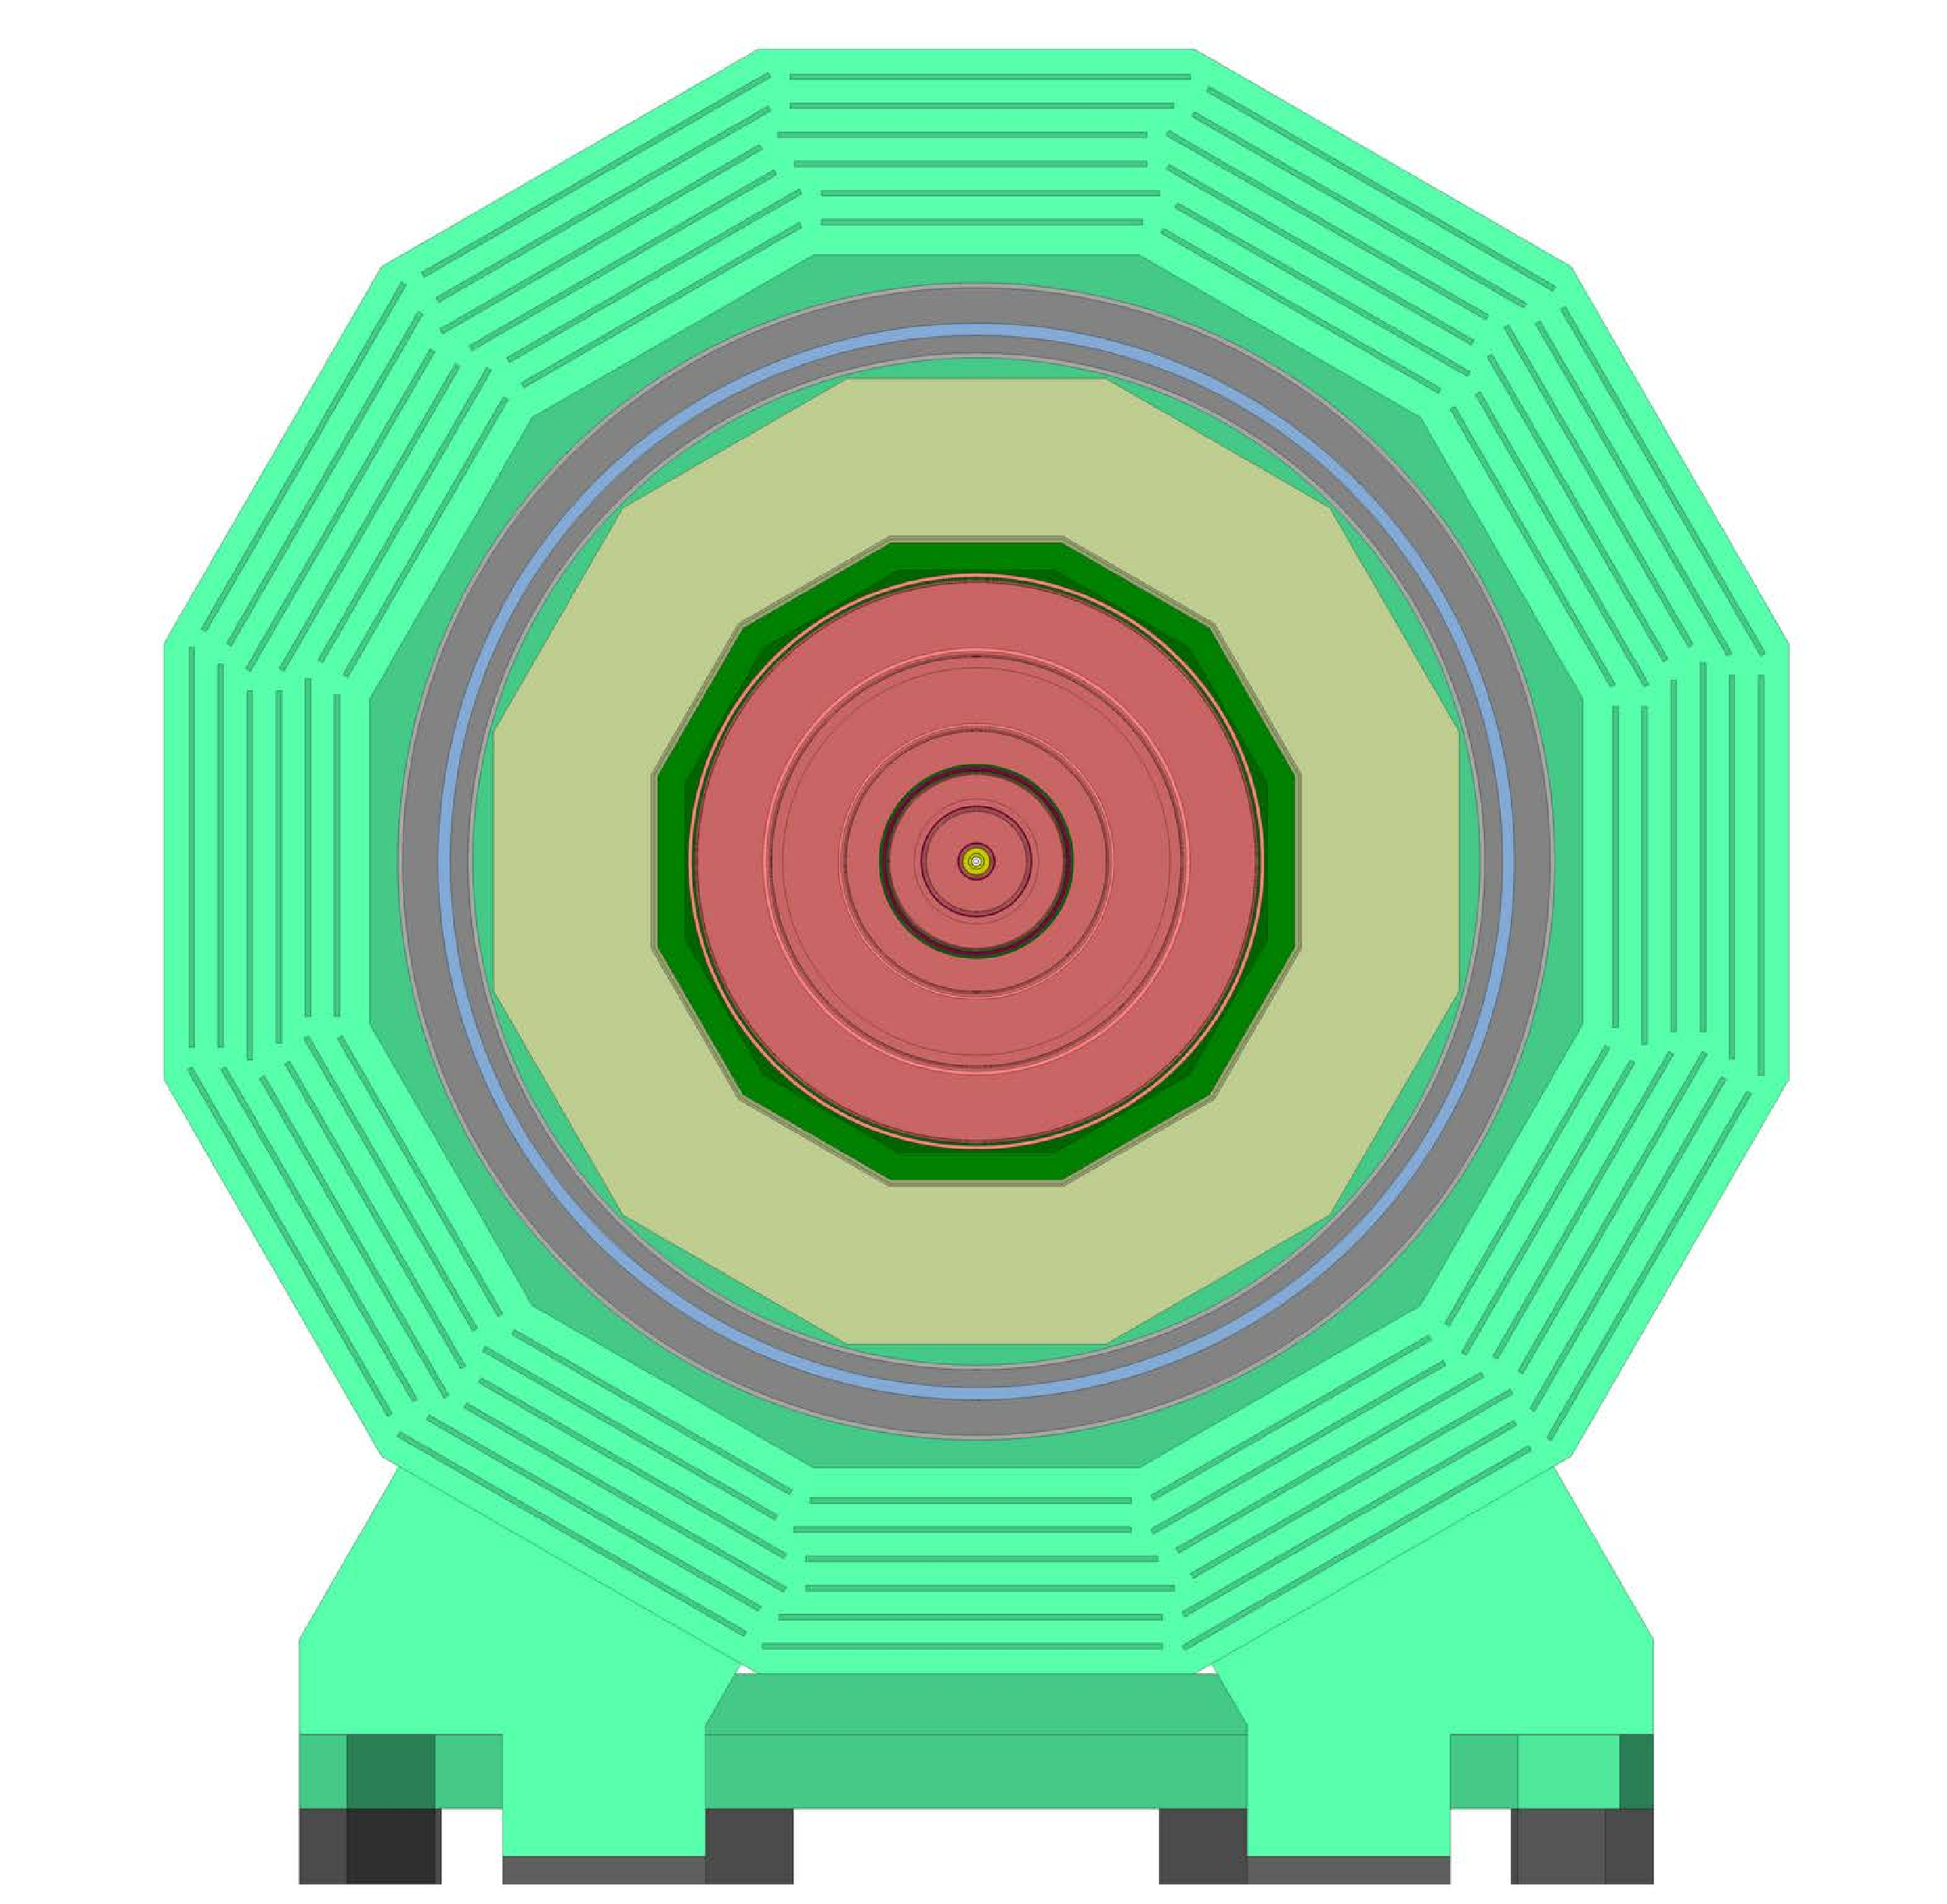
\includegraphics[width=0.51\textwidth]{Physics/DetectorConcepts/Figs/CLD_section.pdf} \hfill
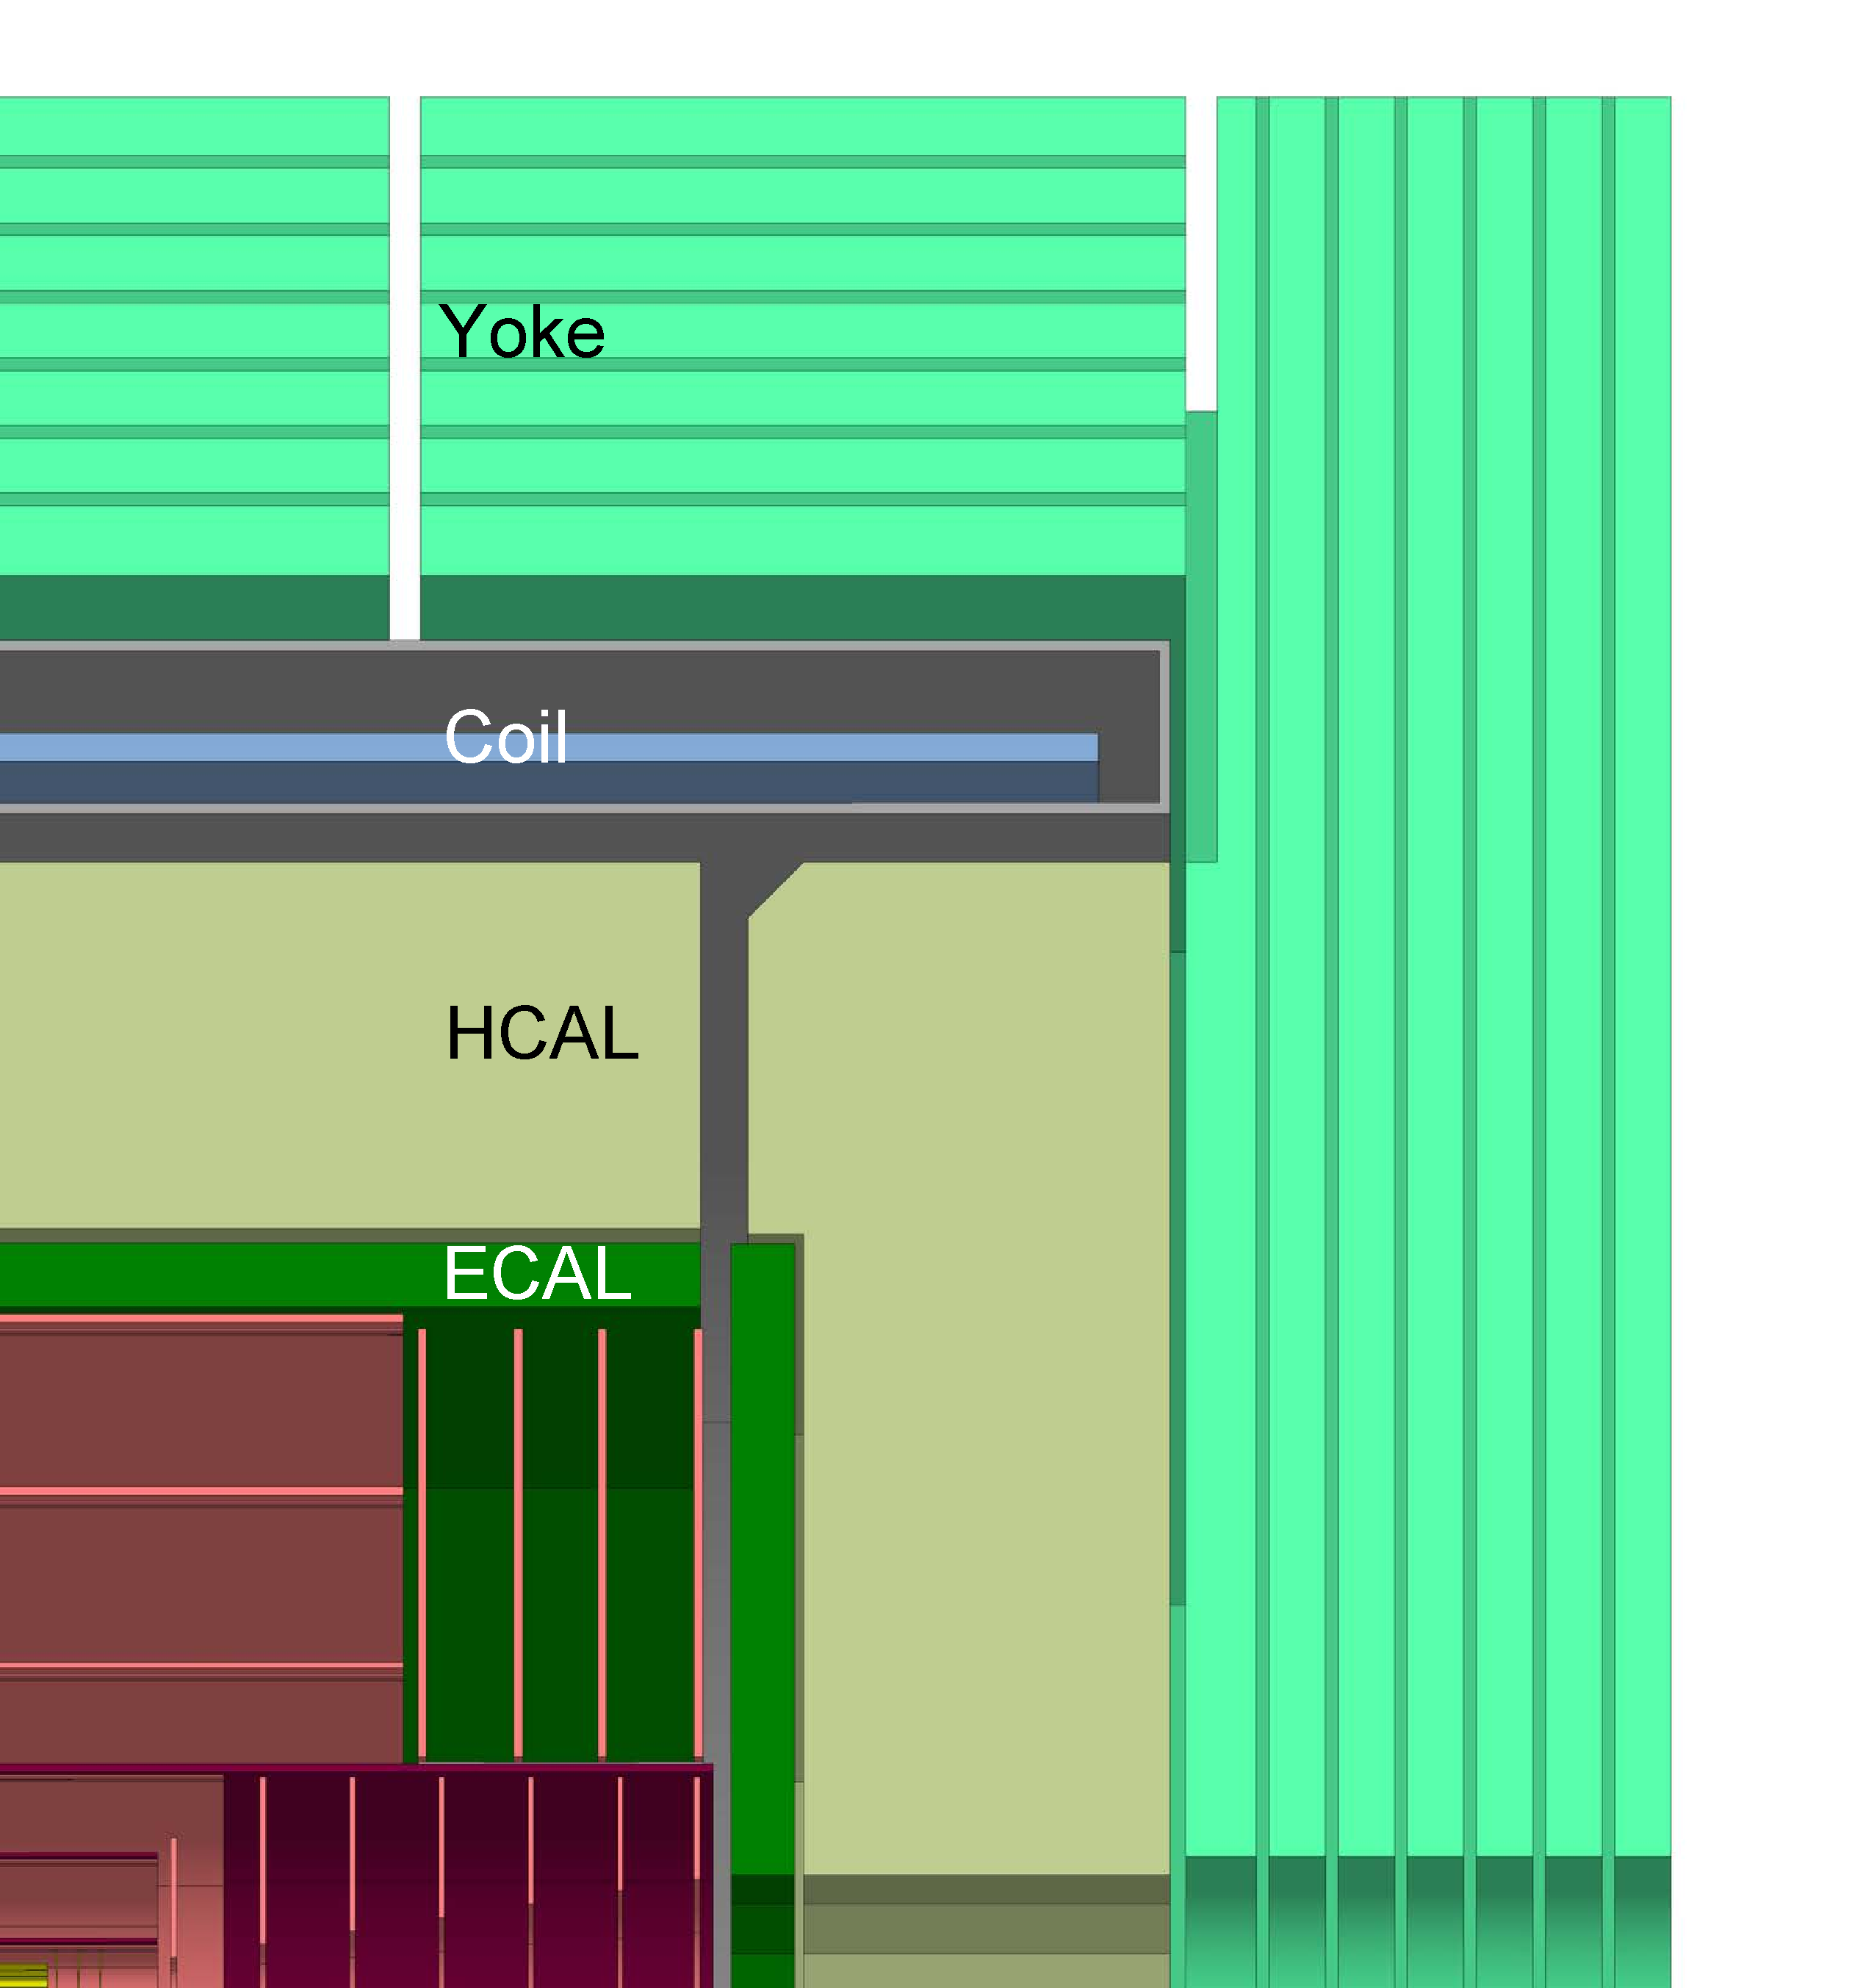
\includegraphics[width=0.48\textwidth]{Physics/DetectorConcepts/Figs/CLD_top_quarter_view.pdf}
\caption{The CLD concept detector: 
end-view cut through (left) and longitudinal cross section of the top right quadrant (right). 
The detector has an overall diameter of 12.0\,m and an overall length of 10.6\,m.}
\label{fig:CLD:detector}
\end{figure}

With respect to the original CLIC detector, 
CLD has an interaction region adapted to the larger crossing angle and 
the more invasive machine-detector interface (Chapter~\ref{sec:mdi}), 
a bigger tracking volume to compensate for the magnetic field limitation of 2\,T, 
and the calorimeter depth adapted to the FCC-ee energy range. 
The tracking system of CLD features a silicon pixel vertex detector (VXD) and a silicon tracker.

A full simulation suite, including full-event reconstruction, 
already exists and provides realistic estimates of full-detector performance figures of merit, 
such as jet resolutions, flavour-tagging efficiencies and purities, background levels, etc. 
Recently, to provide additional handles on particle identification, 
a novel ring-imaging Cherenkov system, ARC~\cite{Forty_ARC, Tat_ARC, forty_2024_6g0gs-7kw30}, 
has been suggested as an extra barrel layer between the tracker and the ECAL;
the tracking system has been correspondingly re-optimised, on the basis of full simulations.

The ILD detector concept is also being studied for a tentative adaptation to FCC-ee. 
It is similarly based on highly granular calorimeter technologies with embedded electronics, 
including silicon pads, monolithic active pixel sensors (MAPS), scintillator strips for the ECAL, 
and scintillator tiles and various gaseous technologies (RPCs, MPGDs) for the HCAL.
Like in the CLD concept, both sections are placed inside the magnet coil. 
The major distinction with CLD is that ILD focuses on a radically different tracking choice, 
a gaseous time projection chamber (TPC), 
favoured for its transparency and particle identification capabilities,
complemented by a surrounding silicon layer to maximise momentum and timing precision. 

The long signal collection times of a TPC, together with the beam-induced background, 
which scales with the high bunch crossing rate, 
raises the question of how reliably a TPC can be operated at FCC-ee, in particular during the Tera-\PZ run. 
This issue is currently being investigated with full-simulation studies using a plug-and-play combination of CLD and ILD, 
which merges the interaction region and inner tracking system of CLD with the ILD TPC and calorimeters.
First results~\cite{DJeansECFA-Paris} indicate that there are distortions due to space-charge effects in the centimetre range. 
Work is ongoing to mitigate these effects 
and possibly demonstrate the feasibility of reaching the performance goals in the \PZ-pole run conditions.

\subsection{The IDEA detector concept} 
\label{sec:IDEADetCon}

The Innovative Detector for $\epem$ Accelerator (IDEA)~\cite{Antonello:2020tzq,Gaudio:2022jve,IDEAStudyGroup:2025gbt},
illustrated in Fig.~\ref{fig:IDEA:detector}, 
is a detector concept specifically designed for FCC-ee, introduced during the Conceptual Design Study~\cite{fcc-ee-cdr}. 
It is based on a silicon pixel vertex detector, a gaseous central tracker, 
and a crystal-based electromagnetic calorimeter placed inside a superconducting solenoidal magnet, 
surrounded by a dual-readout fibre calorimeter and completed by a muon detection system 
placed in the iron yoke that closes the magnetic field. 

\begin{figure}[ht]
\centering
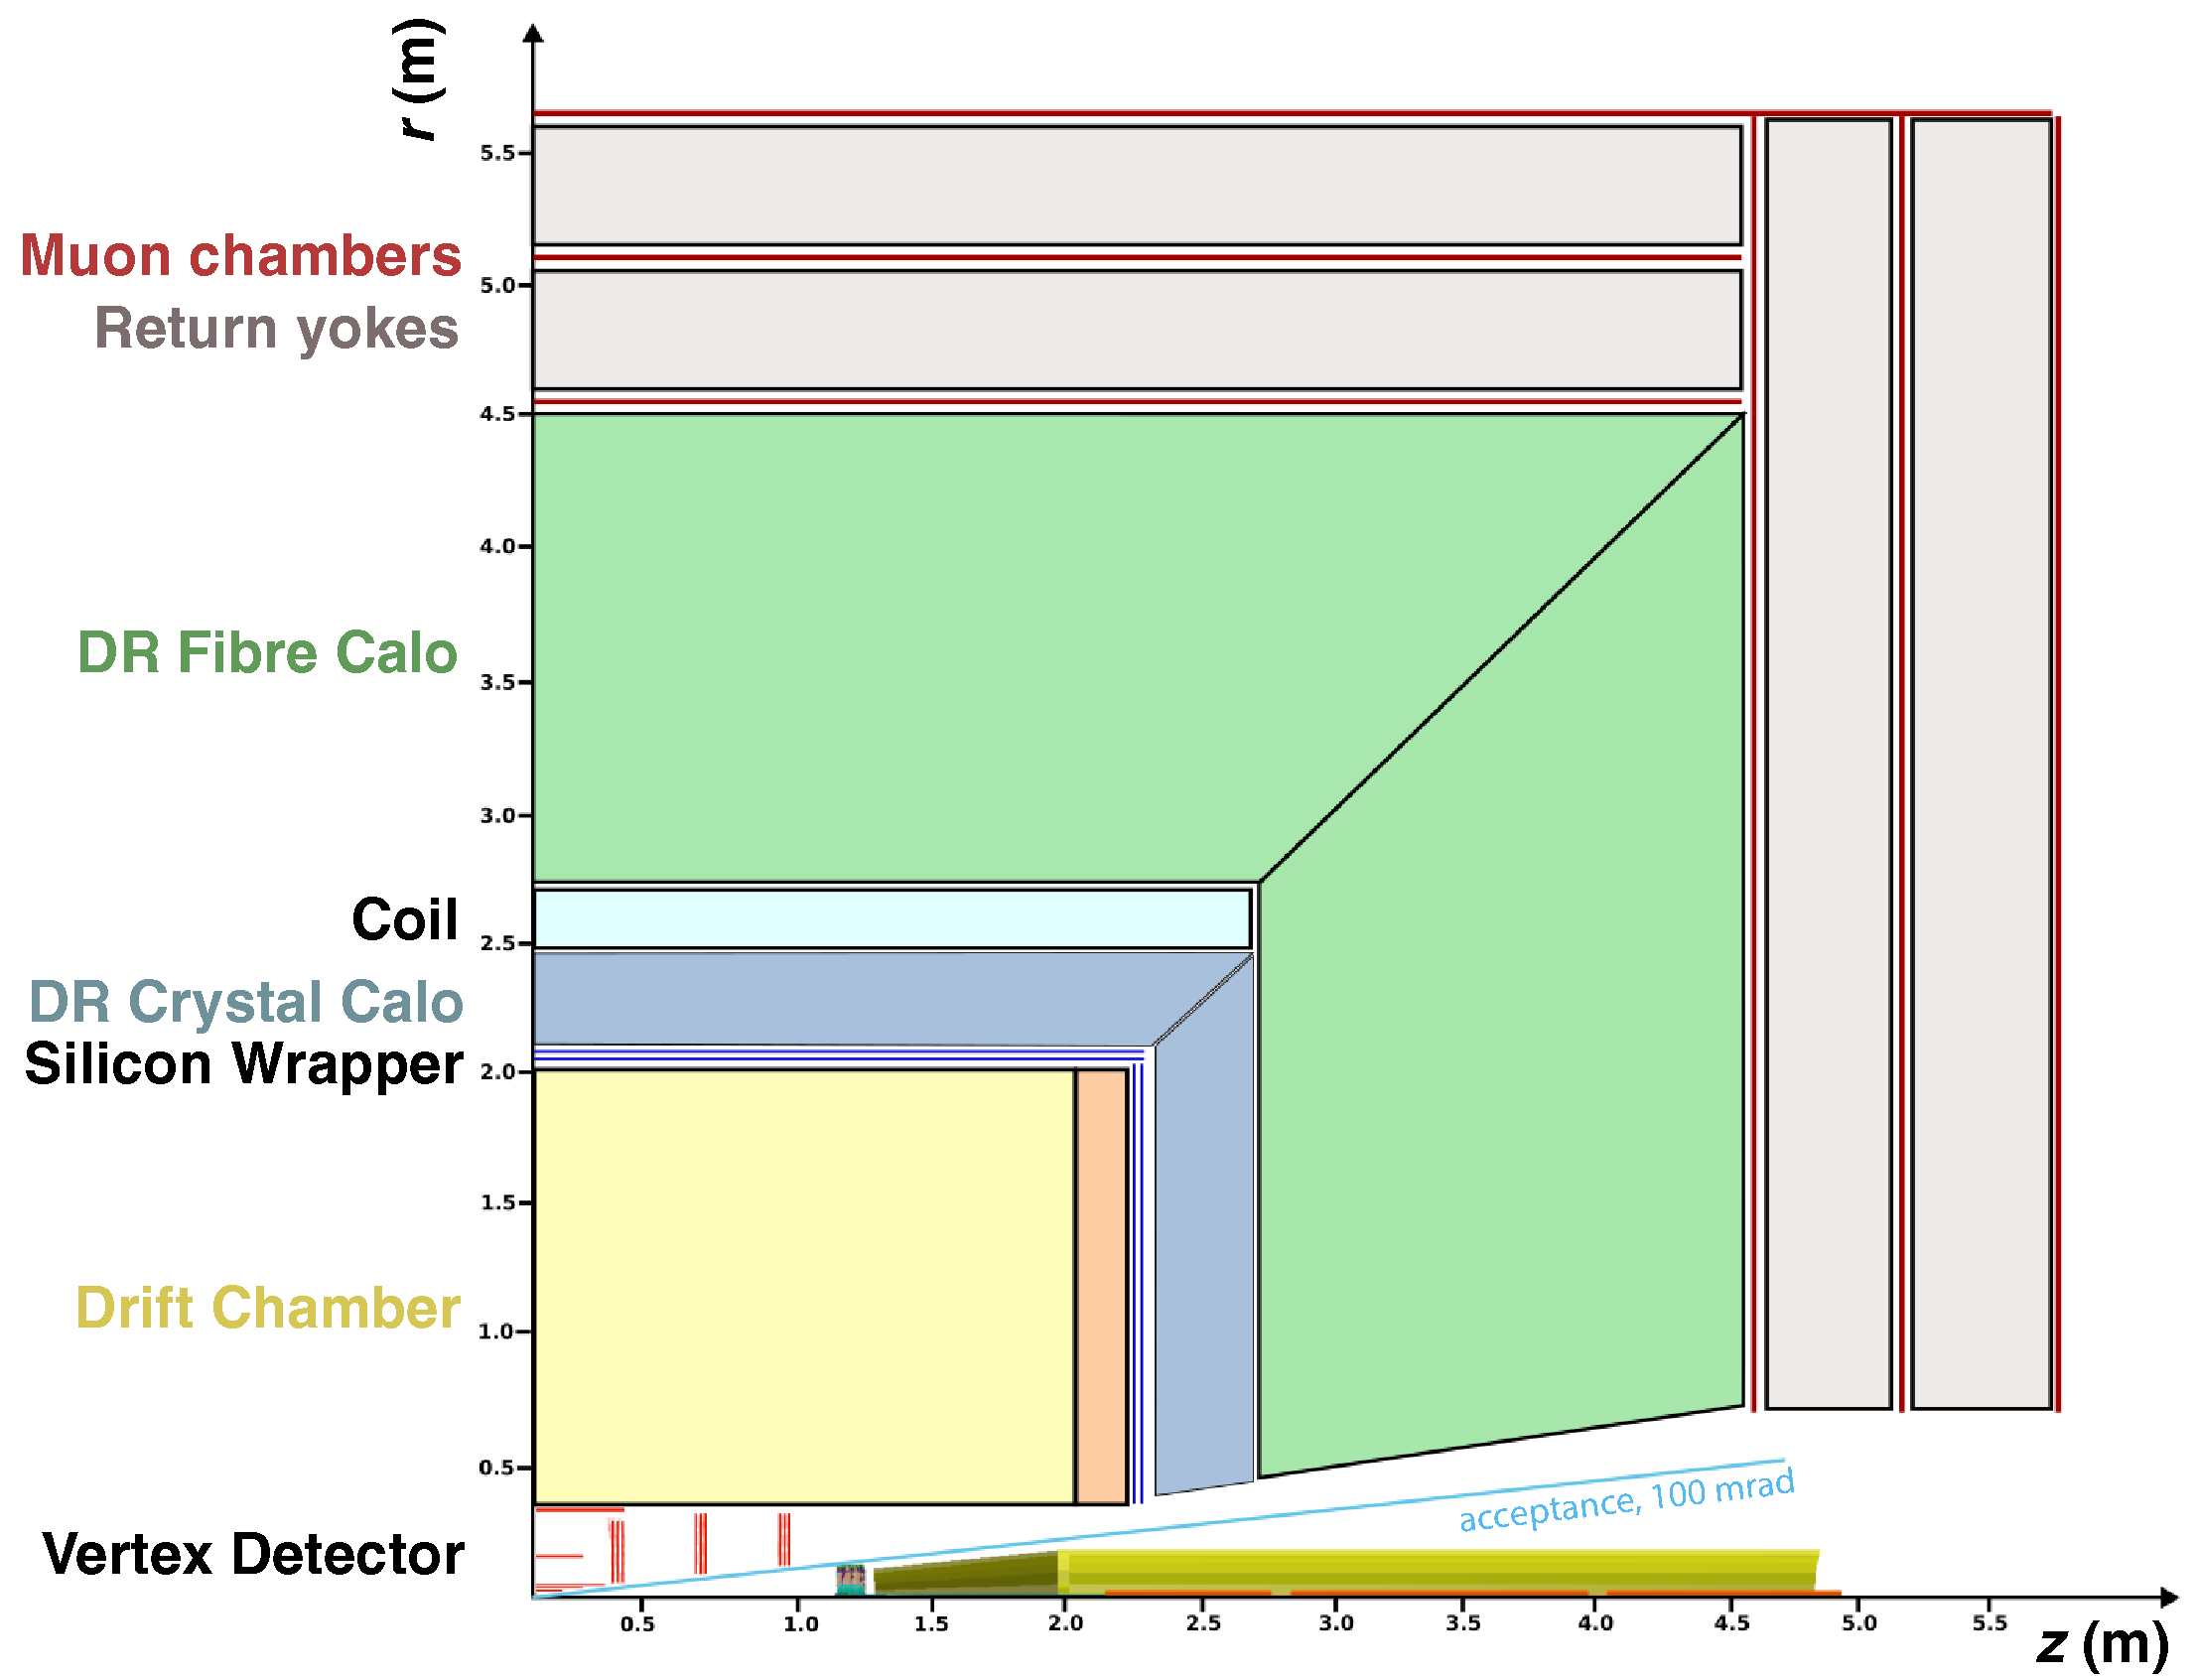
\includegraphics[width=0.75\textwidth]{Physics/DetectorConcepts/Figs/IDEA_baseline_radial_evelope_07_01_2025-v2.pdf}
\caption{Longitudinal cross section of the top right quadrant of the IDEA concept detector.
The LumiCal, the compensating solenoid, and the final-focus quadrupole are displayed along the $z$ axis, 
below the 100\,mrad acceptance line.}
\label{fig:IDEA:detector}
\end{figure}

The tracker is composed of a silicon pixel vertex detector,
a large-volume extremely-light short-drift wire chamber for central tracking and particle identification, 
and a surrounding wrapper made from silicon micro-strip sensors for improved momentum resolution. 
The wire chamber provides up to 112 space-point measurements along a charged particle trajectory 
with particle-identification capabilities provided by the cluster-counting technique. 
Energy resolution for electrons and photons is provided by a finely-segmented crystal electromagnetic calorimeter. 
The particle identification capabilities of the drift chamber are complemented by a time-of-flight measurement, 
provided either by LGAD technologies in the Si wrapper or by a first layer of LYSO crystals in the ECAL. 
Outside a thin (about 30\,cm thick) low-mass (corresponding to less than 0.8\% of a radiation length) superconducting solenoid, 
the calorimeter system is completed by a dual readout fibre calorimeter, 
providing enhanced energy precision for isolated hadrons and hadron showers, 
and a return path for the magnetic field. 
The muon detection system is based on the \mbox{$\mu$-Rwell} detectors, 
a recent micro-pattern gas detector that provides a space resolution of a few hundred microns, 
giving the possibility of reconstructing secondary vertices at a large distance from the interaction point. 

\subsection{The ALLEGRO detector concept}
\label{sec:ALLEGRODetCon}

The ALLEGRO (A Lepton-Lepton collider Experiment with Granular Read-Out) detector concept 
is relatively recent and under rapid development.
Its design, illustrated in Fig.~\ref{fig:allegro_concept}, 
is articulated around a high-granularity noble liquid electromagnetic calorimeter in a cryostat made from novel lightweight materials, 
thus taking advantage of the excellent stability of this technology, 
and it capitalises on recent progress in electronics integration and advanced mechanical structures. 
The inherent linearity, stability, and uniformity of noble liquid calorimeters 
allow exquisite control of systematic uncertainties, a unique asset for high-precision measurements. 

\begin{figure}[ht]
\centering
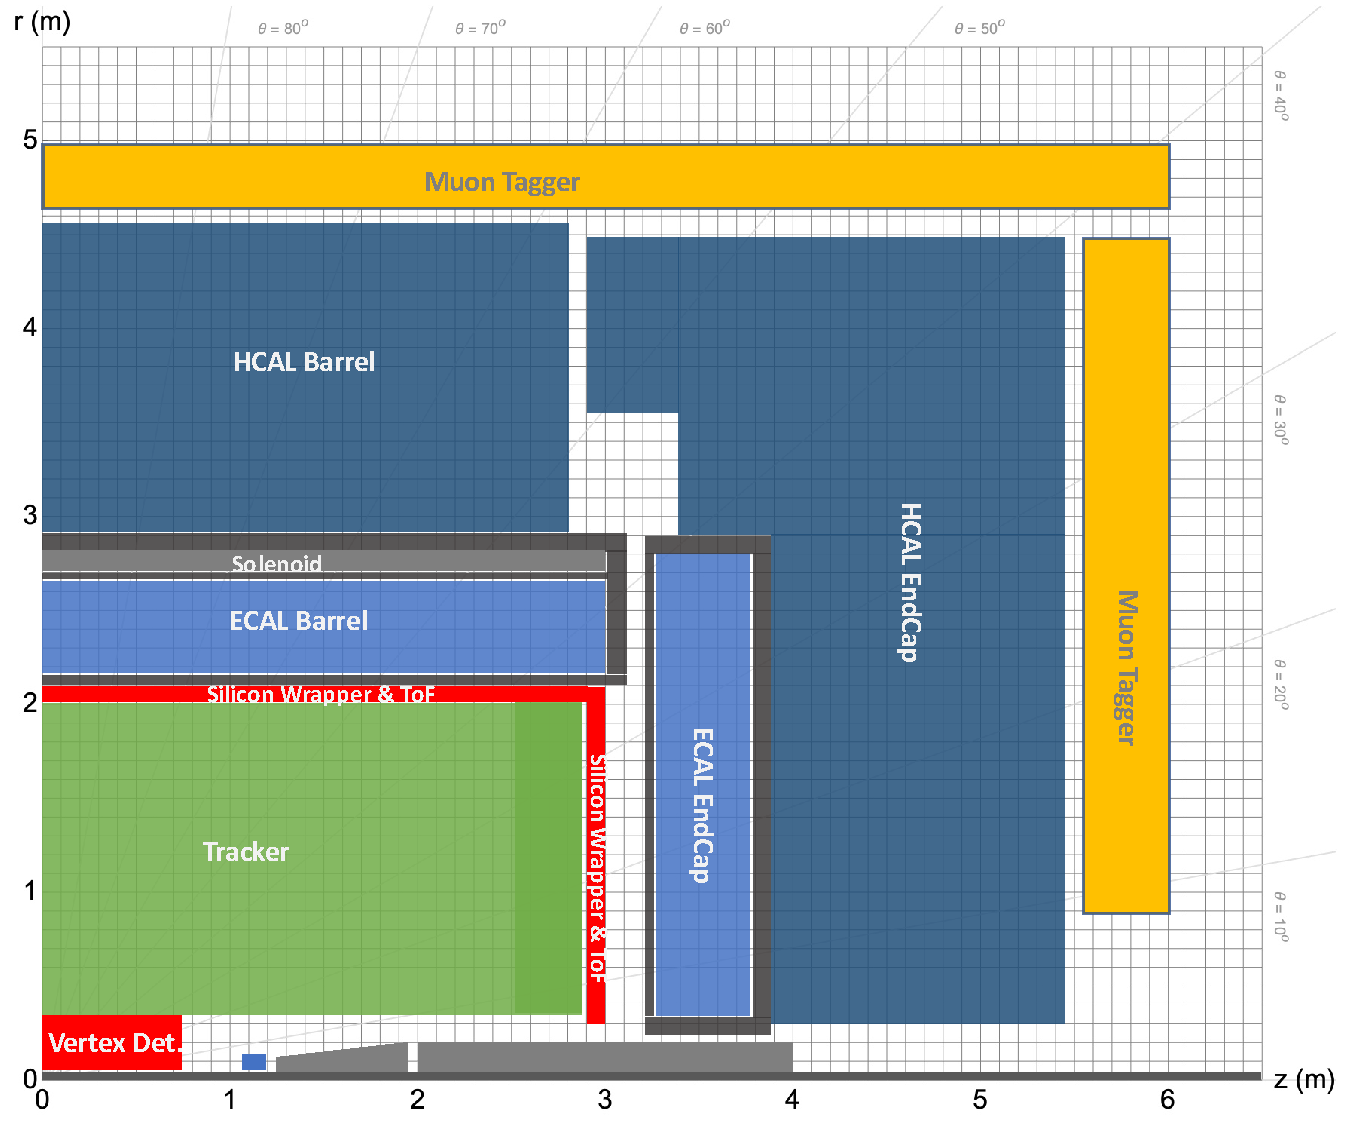
\includegraphics[width=0.6\textwidth]{Physics/DetectorConcepts/Figs/ALLEGRO-concept.pdf}
\caption{Longitudinal cross section of the top right quadrant of the ALLEGRO concept detector.
The LumiCal, the compensating solenoid, and the final-focus quadrupole are displayed along the $z$ axis.}
\label{fig:allegro_concept}
\end{figure}

The tracking system consists of a silicon vertex detector and a main tracker that remains to be identified. 
The silicon vertex detector is expected to use  MAPS or DMAPS technology, 
with the possible inclusion of an LGAD layer for precise timing measurements. 
Both a drift chamber and a straw layer are considered for the gaseous tracker option.
If a gaseous tracker is chosen, a silicon wrapper is foreseen at the outer periphery of the tracking volume,
to provide precise track measurements at the entrance of the calorimeter
and possibly a precise measurement of the time of flight by using LGAD technology.
A fully silicon-based tracking system, like in CLD, is also being considered 
and is used in full-simulation particle-flow studies. 

A high-granularity-sampling noble liquid ECAL surrounds the tracker. 
The options considered consist of lead (or tungsten) and liquid argon, or tungsten and liquid krypton.  
The use of innovative, low-power, cold front-end electronics, placed inside the cryostat, could provide a noiseless readout, 
but the option of placing low-noise electronics outside the cryostat is also being studied. 
The thin, lightweight coil is located around the ECAL, within the same cryostat. 
The high-granularity HCAL
is made of steel absorber plates interleaved with scintillator tiles, 
corresponding to at least 8 interaction lengths.
Two design options are being considered, 
one with SiPMs directly coupled to the scintillating tiles (as for CLD), 
and the other with wavelength-shifting (WLS) fibres used to guide the light to SiPMs located outside the detector (as for the ATLAS HCAL).
The HCAL also acts as a return yoke for the magnetic field.

The geometry described above, with a barrel and two end-caps, is considered as a `baseline'.
An alternative layout is also being considered, 
with a somewhat longer barrel and the end-caps replaced by smaller radius end-plugs fitting in the barrel opening. 
This solution would provide several engineering advantages, 
including the routing of the cables in and out of the barrel cryostat
and the reduction of the gap-widening issue in the end-cap ECAL modules. 

For the muon system, several options are under consideration,
including drift tubes or chambers, resistive plate chambers (RPCs), and micromegas (MM). 
Here, the development of eco-friendly but performant gas mixtures is a compelling line of R\&D.

\subsection{Vertex detectors}
\label{sec:IDEA_vertex}

Vertex detector design is undergoing a strong technological development that can be summarised by the terms \emph{lighter}, \emph{closer}, and \emph{more precise}.  
The development is driven by upgrade activities in Belle~II and in the LHC experiments. 
The second and third generation ALICE vertex detectors, ITS2 and ITS3~\cite{Mager:2747243}, are of particular relevance for FCC-ee,
with many common conditions and requirements, such as moderate radiation environments and the need for high resolution and low multiple scattering. 
The technology of choice, CMOS MAPS, can be thinned down to a thickness of 50\,$\mu$m or less, 
so that the sensors can ultimately be bent into cylindrical layers around the beam pipe with very little support material. 

A comprehensive description of the silicon vertex detector, considered for the IDEA and ALLEGRO detector concepts, is presented in this section. 
This detector element is currently the most advanced from an engineering point of view, 
being already integrated in the complex Machine Detector Interface layout (Chapter~\ref{sec:mdi}). 
A much briefer description of the vertex detector considered for CLD follows.

The vertex detector considered for IDEA and ALLEGRO features two main subsystems,  
whose active elements are based on 50\,$\mu$m thick MAPS:
\begin{itemize}
\item an inner detector, 
located close to the beam pipe, at radii between 13.7 and 35.6\,mm, 
covering an angular acceptance of about $|\cos\theta| < 0.99$;
\item an outer detector, located at radii between 130 and 315\,mm, 
composed of a middle barrel, an outer barrel, and three disks on each end-cap.
\end{itemize}

Two layouts are being explored for the inner vertex detector.
The baseline layout uses a traditional approach, 
with modules mounted on a carbon fibre support structure.
An alternative, less advanced, ultra-light layout is based on curved detectors, 
using a concept similar to the ALICE ITS3~\cite{Mager:2747243}.
The baseline layout of the vertex detector is displayed in Fig.~\ref{fig:Vertex_all}.

\begin{figure}[ht]
\centering
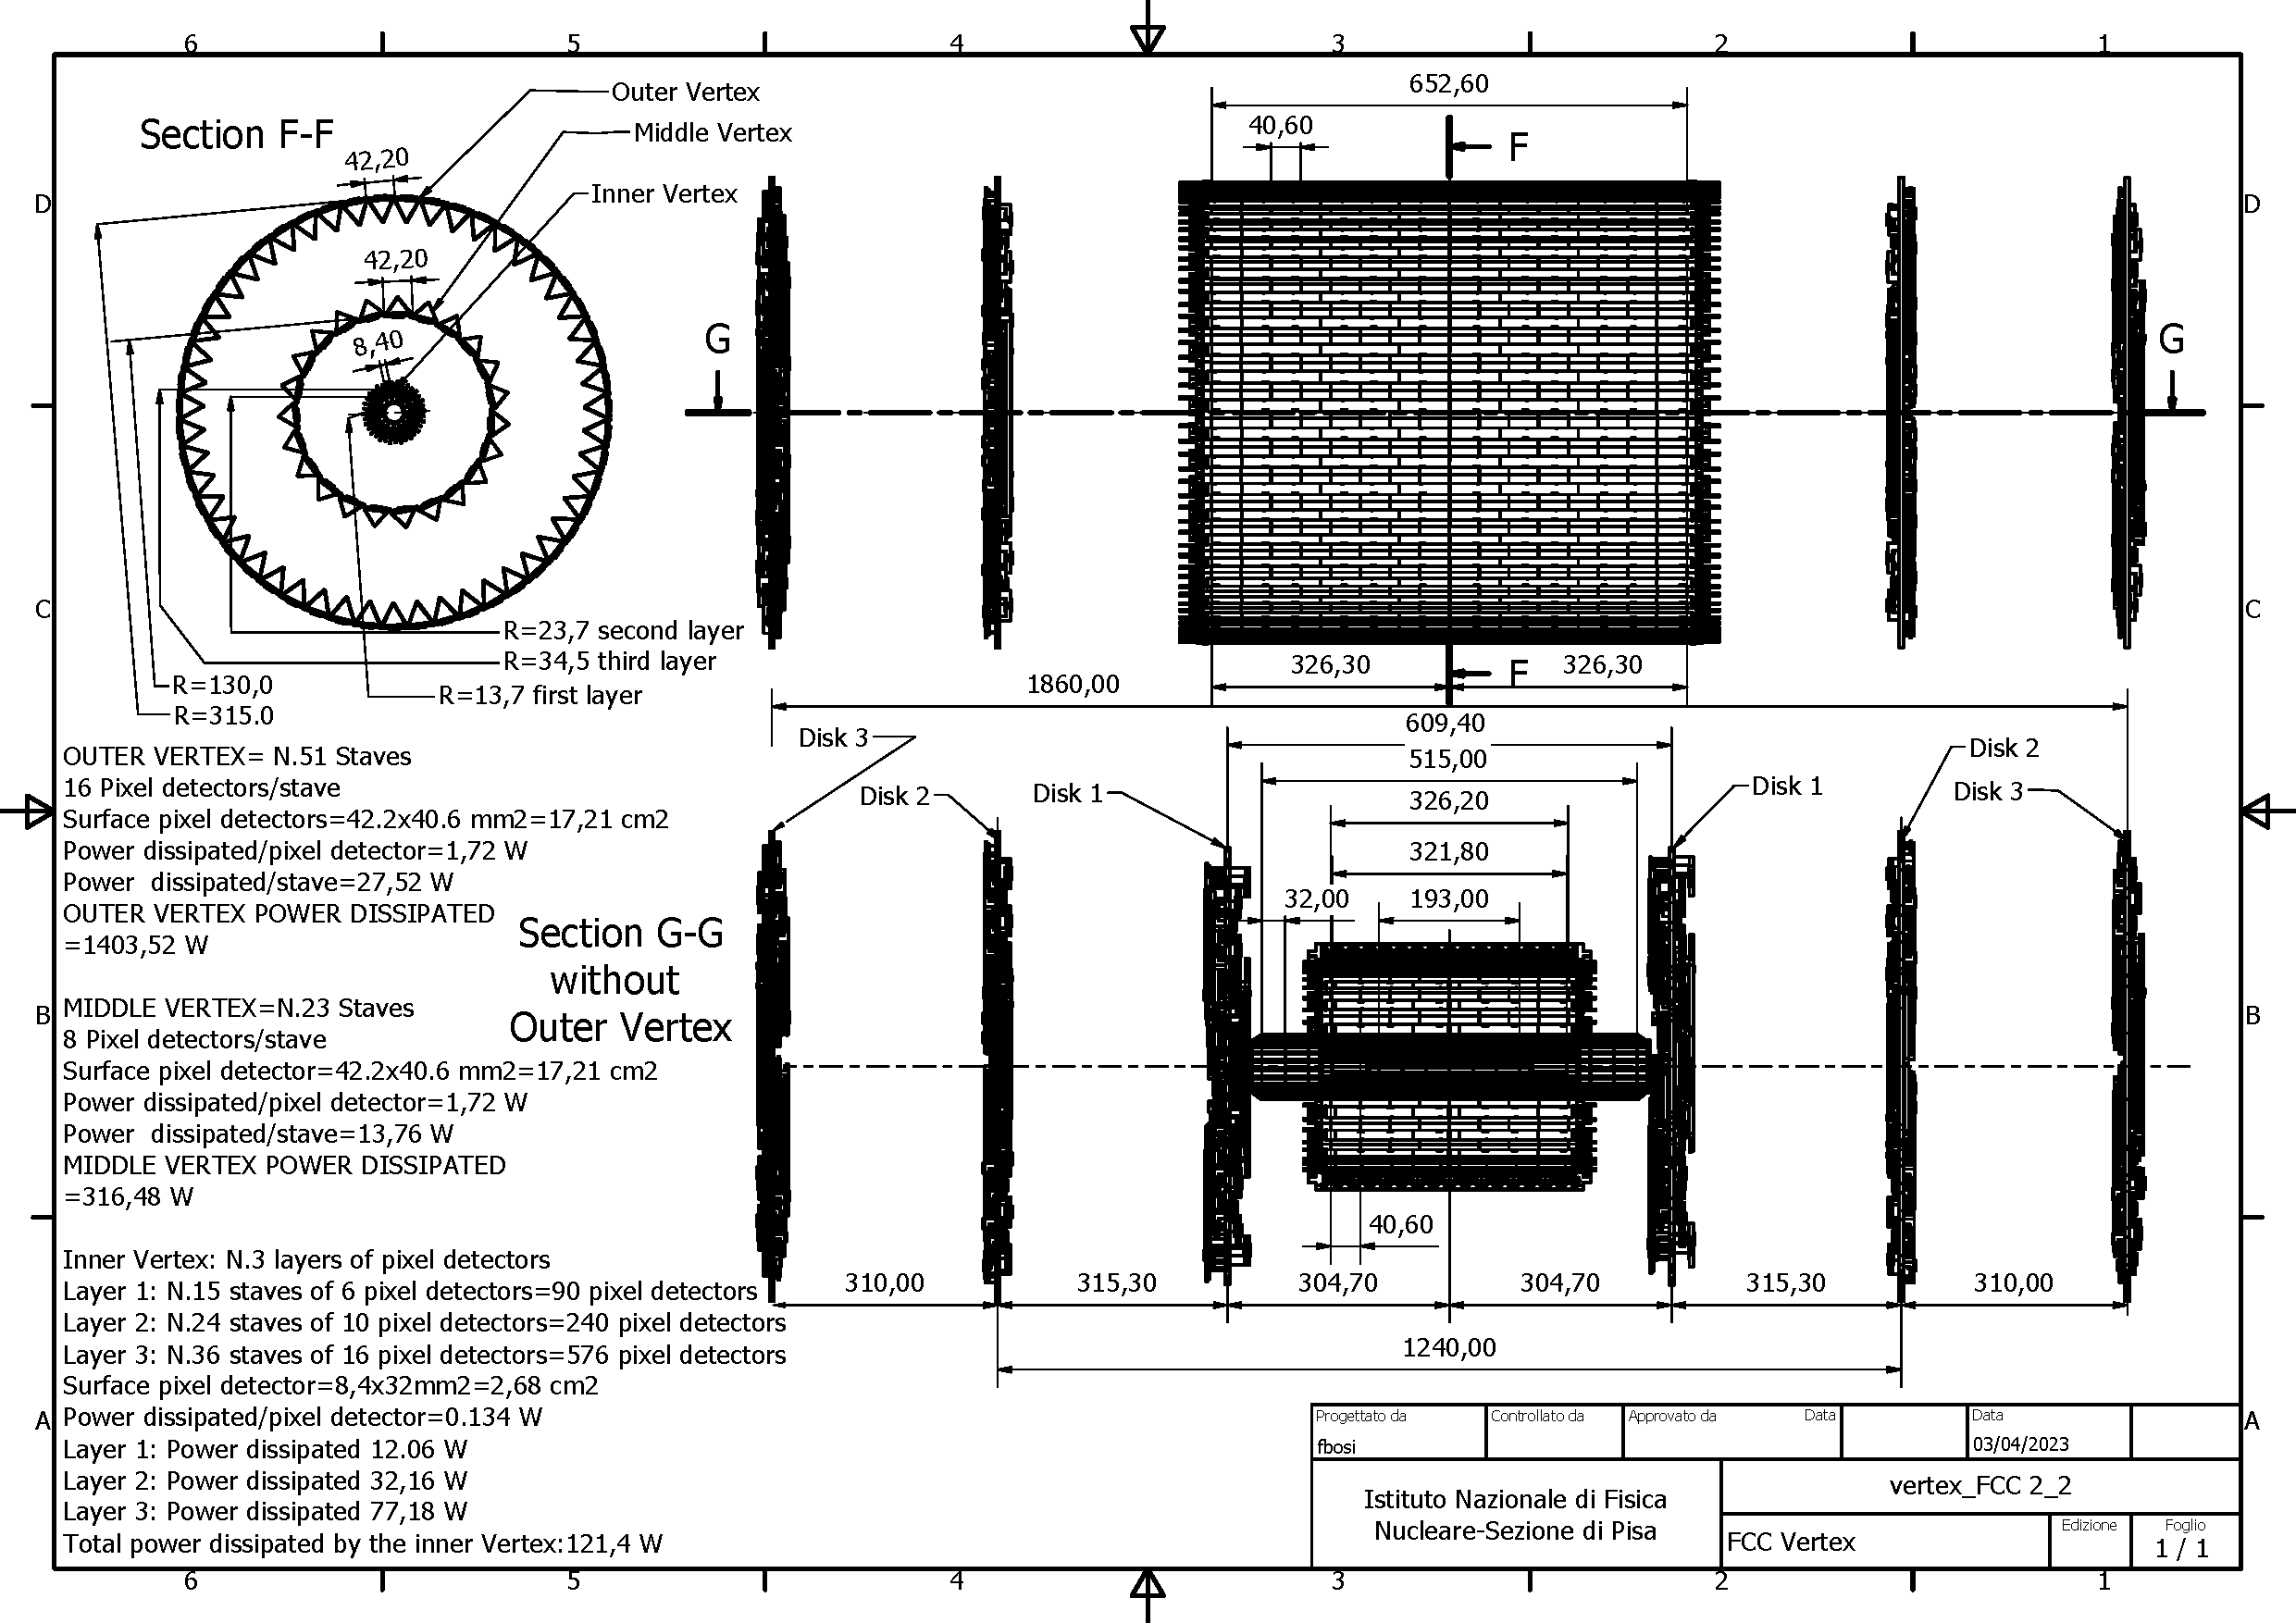
\includegraphics[width=0.995\linewidth]{Physics/DetectorConcepts/Figs/assieme-middle-outer-e-inner-tracker_2_2.pdf}
\caption{Engineered layout and main characteristics of the baseline vertex detector for the IDEA and ALLEGRO detector concepts. 
Top-left: Cross sectional view showing the barrel layers. 
Top-right: Longitudinal view showing the outer barrel and disks.
Bottom-right: Longitudinal view with the inner and middle barrels, as well as the disks. 
All dimensions are in mm. 
The bottom-left panel lists the main elements for the outer, middle, and inner barrel detectors,
together with the dissipated power.}
\label{fig:Vertex_all}
\end{figure}

In the baseline layout, the inner vertex detector is composed of three concentric barrel layers 
mounted on a carbon fibre structure. 
The elementary unit is a module of $32 \times 8.4$\,mm$^2$ $z \times r\phi$ dimensions. 
Each module has two chips abutted together in $z$, inspired from the ARCADIA R\&D~\cite{ARCADIA}. 
The chip active area features $640\,(z) \times 256\,(r\phi)$ pixels 
of $25 \times 25$\,$\mu$m$^2$ area. 
A 2\,mm inactive space is envisaged in $r\phi$, corresponding to the periphery of the chip. 
A conservative power consumption of 50\,mW/cm$^2$ is assumed, 
based on the $\sim$\,30\,mW/cm$^2$ measured for the current ARCADIA prototype, read out at 100\,MHz/cm$^2$, 
and considering the higher expected FCC-ee data rate.
In order to allow for a 2\,mm radial clearance in view of its insertion, 
the first layer is located at a radius of 13.7\,mm. 
The length is constrained by the central beam pipe cooling manifolds. 
The first layer comprises 15 staves with 6 modules each, along $z$. 
The staves overlap in $\phi$, as shown in Fig.~\ref{fig:layer1}, to allow internal alignment.

\begin{figure}[ht]
\centering
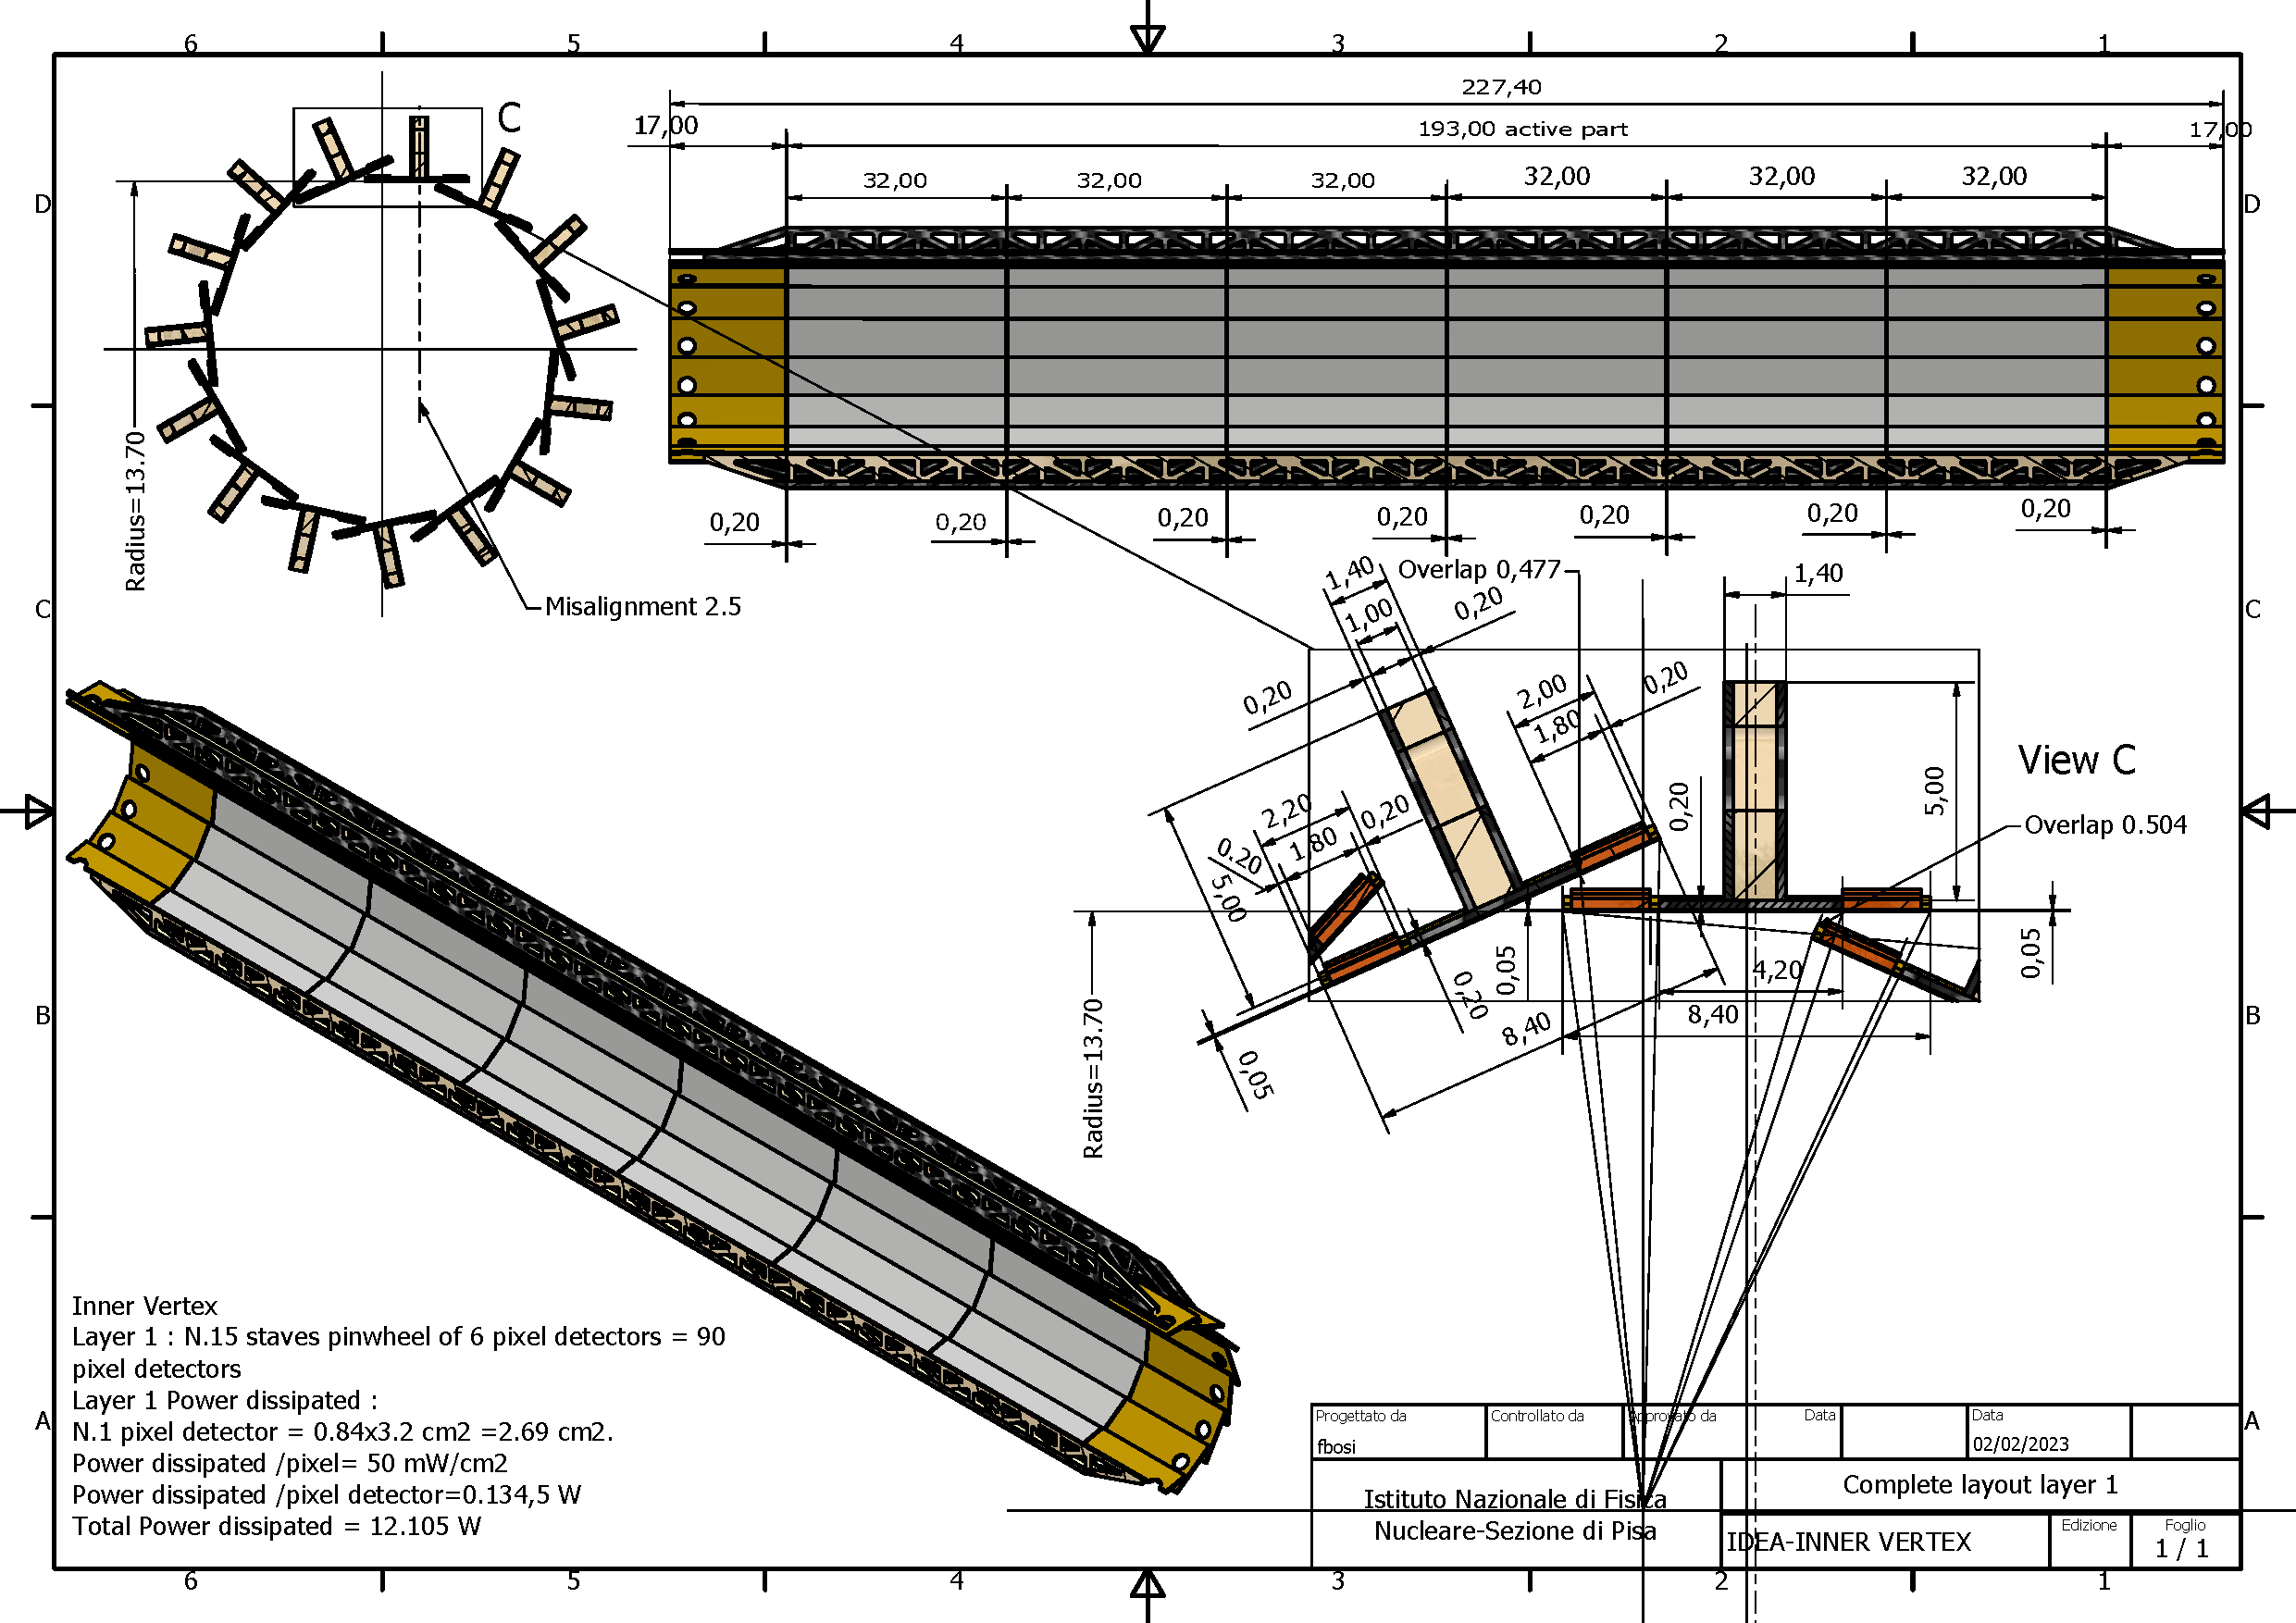
\includegraphics[width=0.99\linewidth]{Physics/DetectorConcepts/Figs/Assieme-completo-definitivo-layer1-piatto-bus-stretto_2.pdf}
\caption{First layer of the baseline inner vertex detector for the IDEA and ALLEGRO detector concepts.
Transverse (top-left) and longitudinal (top-right) cross sections of the assembly;
3D view (bottom-left); 
and detailed view showing the overlaps and the different structures (bottom-right). 
All dimensions are in mm.
The 50\,$\mu$m thick MAPS sensors face the centre of the structure. 
The brown structures are the buses and the golden parts are the electronic hybrid circuits for readout.}
\label{fig:layer1}
\end{figure}

A lightweight support on each ladder provides rigidity and facilitates the mounting of the MAPS. 
The structure is made of thin carbon fibre walls interleaved with Rohacell~\cite{Rohacell}, 
which holds the sensors (facing the beam pipe) 
and two 1.8\,mm wide buses (one for data, the other for power) at the edges of the structure.
The thickness of the bus comprises 200\,$\mu$m Kapton and 50\,$\mu$m aluminium, for a total of 0.09\%\,$X_0$. 
The ladders are arranged in a pin-wheel geometry.

The second layer, with a structure similar to the first, 
is made of 24 ladders of 10 modules each, at a radius of 23.7\,mm, 
arranged in a pin-wheel geometry opposite in orientation to that of the first layer, 
to mitigate possible charge-dependent effects on charged-particle track reconstruction.
The third layer has 36 ladders, each composed of 16 modules. 
The ladders are arranged in a $\phi$-symmetric lampshade fashion: 
half of the ladders are located at a radius of 34\,mm, the other half at 35.6\,mm. 
Each layer contributes $0.25\%$\,$X_0$ at normal incidence, 
about one fifth of it coming from the overlap between staves of the same layer.
The vertex detector layers are mounted on conical carbon fibre support structures 
using two rings of peek material for thermal isolation during bakeout.
The conical support structures also guide cooling gas inside the detector volume 
and support the power and readout circuits.
The middle barrel and the disks, together with the support cones, 
are shown in Fig.~\ref{fig:cooling_cones} (Chapter~\ref{sec:mdi}). 
The amount of detector material crossed by a particle originating from the main IP 
(`material budget') is shown in Fig.~\ref{fig:baseline_vtx_material_budget}, 
for the inner vertex layers and for the complete vertex detector.

\begin{figure}[ht]
\centering
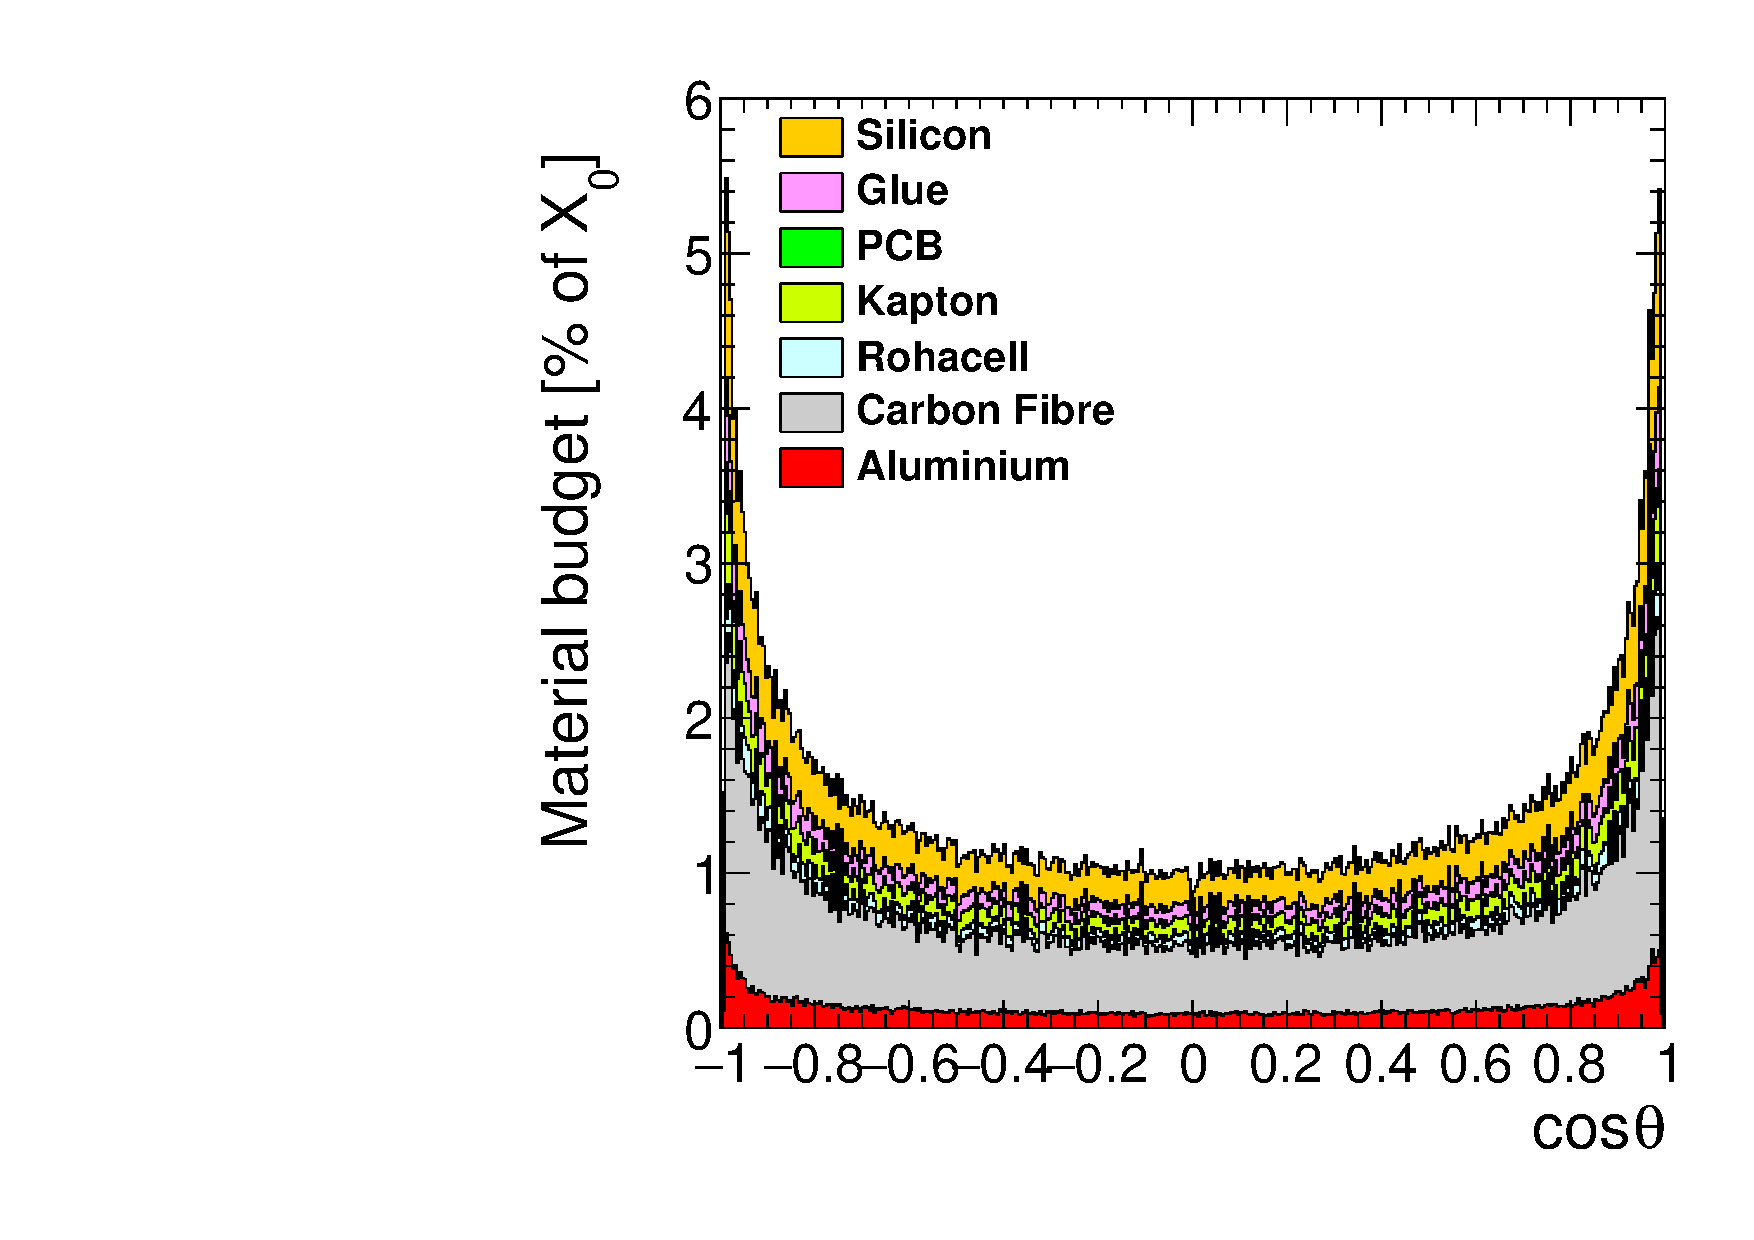
\includegraphics[width=0.46\textwidth]{Physics/DetectorConcepts/Figs/inner-vertex-1d-x0.pdf}
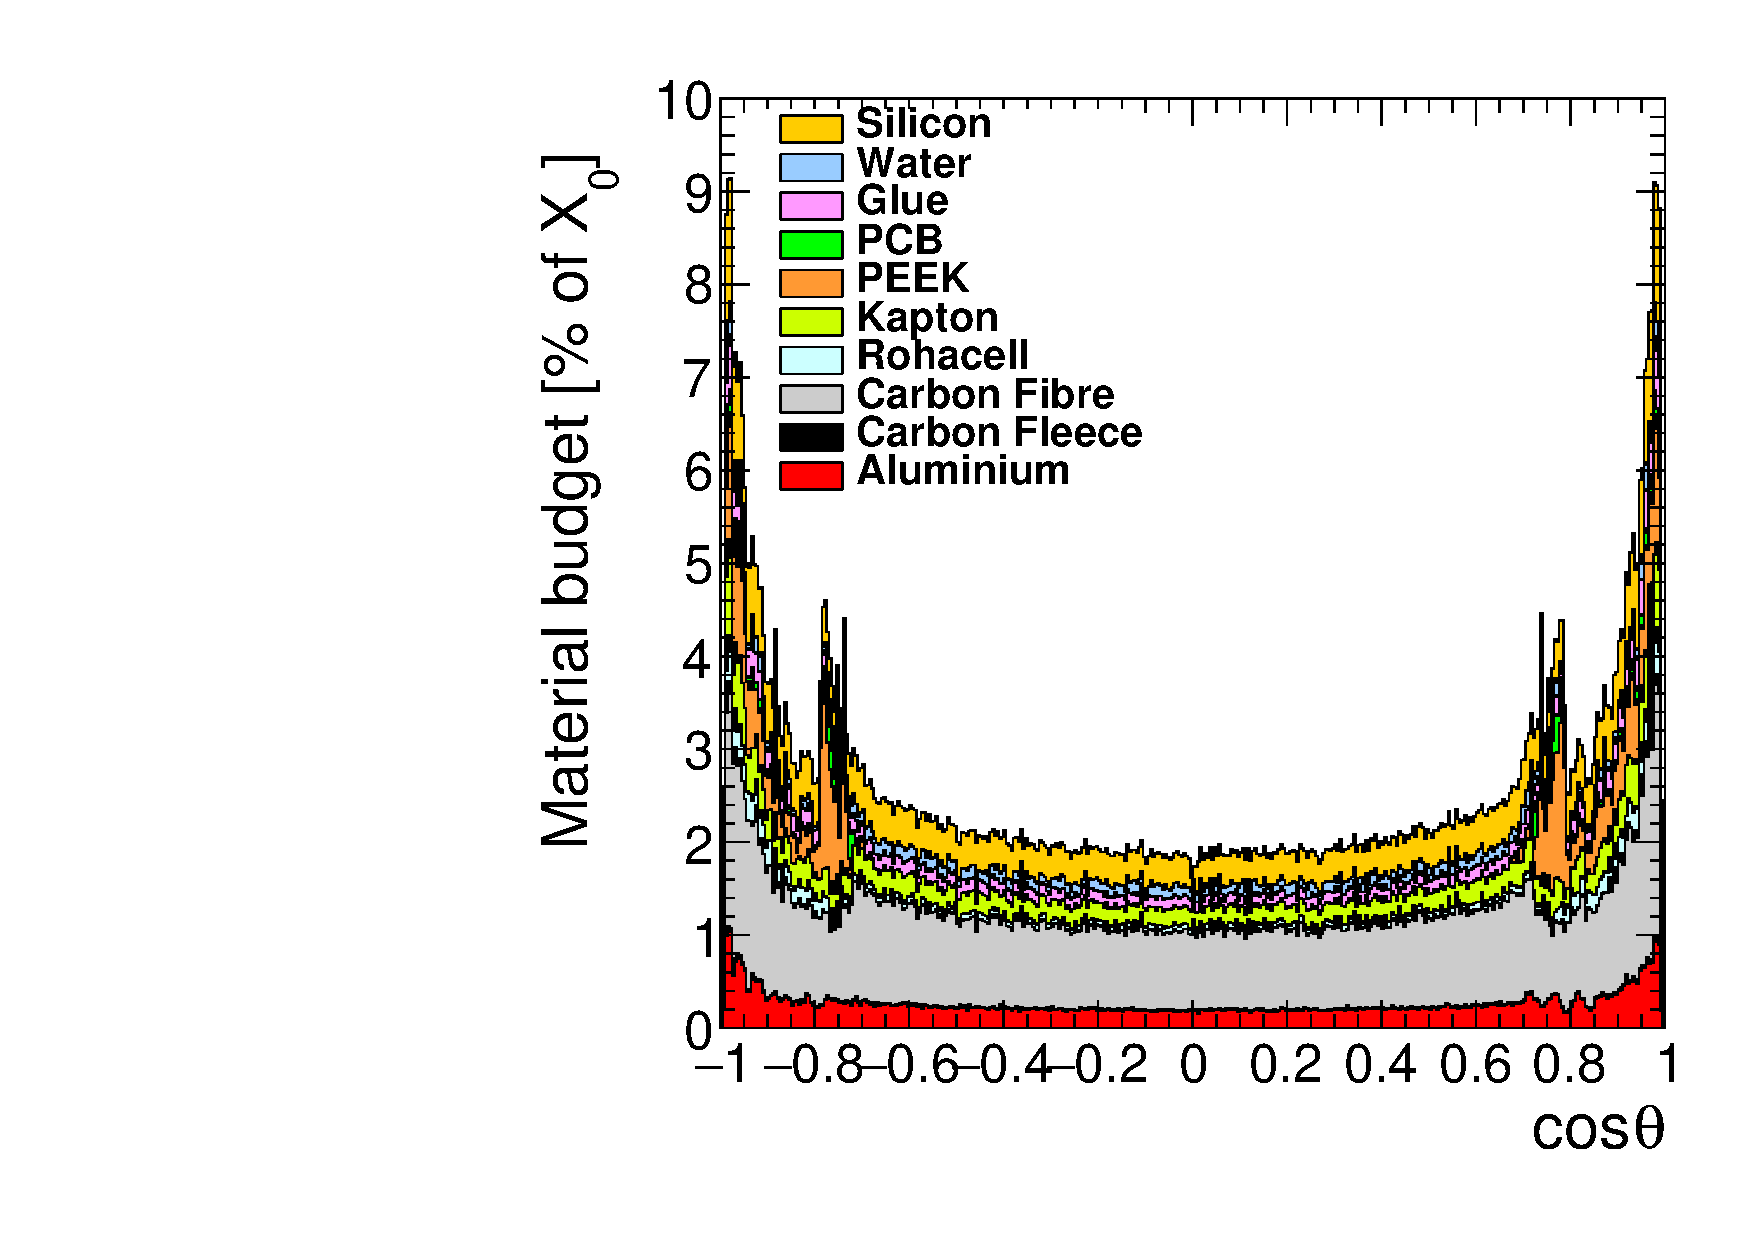
\includegraphics[width=0.46\textwidth]{Physics/DetectorConcepts/Figs/Vertex_x0_1D_-1_to_1.pdf}
\caption{Material budget (expressed as a percentage of a radiation length) 
for the silicon vertex detector considered for ALLEGRO and IDEA for the inner vertex detector (left) 
and for the complete vertex detector (right), 
in the baseline design, as a function of the cosine of the polar angle.}
\label{fig:baseline_vtx_material_budget}
\end{figure}

The main geometric dimensions of the vertex detector, 
together with the power dissipated by each layer, 
are reported in Table~\ref{tab:vertex_details}. 
The inner vertex detector is planned to be cooled with gas passing through channels embedded in the conical support structure. 
Both atmospheric air and helium are considered as coolant gases. 
The gas is contained in a cylindrical, 200\,$\mu$m thick, carbon fibre envelope surrounding the detector.
The cooling performance has been analysed using computational fluid dynamics (CFD) simulation models, 
and the result is that the largest temperature difference between the modules along a stave 
is less than 15\,$^\circ$C.
Although this is considered an acceptable level,
further optimisations are ongoing to reduce this temperature difference.
A mechanical vibration analysis based on Finite Element Analysis (FEA) in ANSYS
showed a maximum displacement amplitude in the radial direction of about 1.5\,$\mu$m 
for a nominal air flow of 0.7\,g/s,
resulting in a negligible effect on the impact-parameter resolution.

\begin{table}[t]
\caption{Main parameters of the baseline vertex detector considered for the IDEA and ALLEGRO detector concepts.}
\centering
\footnotesize
\begin{tabular}{l c c c c c c}
\toprule
Subsystem & Layer ID & Radius (mm) & $|z|$ (mm) & No.\ staves & No.\ modules / stave & Power (W) \\
\midrule
Inner barrel & 1 & 13.7 &  $<96.5$ & 15 & 6 & 12\\
Inner barrel & 2 & 23.7 &  $<160.9$ & 24 & 10 & 32\\
Inner barrel & 3 & 34 and 35.6 & $<257.5$ & 36 & 16 & 77 \\
\midrule
Middle barrel & 1 & 130 & $<163.1$ & 23 & 8 & 316\\
Outer barrel & 2 & 315 &  $<326.3$ &  51 & 16  & 1400\\
\midrule
Disks & 1 & $34.5 < r < 275$ & 304.7 & 56 & 2--6 & 135\\
Disks & 2 & $70 < r < 315$ & 620 &   48 & 3--7 & 420\\
Disks & 3 & $105 < r < 315$ & 930 &  40 & 4--7 & 370\\
\bottomrule
\end{tabular}
\label{tab:vertex_details}
\end{table}

A second, ultra-light layout for the inner vertex detector is being explored, albeit with a less advanced system engineering. 
The layout is based on a concept similar to the ALICE ITS3 curved sensor technology, 
which facilitates a self-supporting structure with essentially no material besides that of the Si sensors. 
The ITS3 uses a stitching technique to form wafer-scale sensors from multiple repeated sensor units (RSUs). 
Each layer comprises two half-cylindrical sensors featuring ten RSUs in $z$ 
and three, four, or five in $\phi$ for the first, second, and third layers, respectively.
Unlike ITS3, a vertex detector for FCC-ee must have the largest possible polar-angle coverage. 
The inner vertex detector has four layers, 
of which the first three are arranged to have approximately the same angular acceptance 
while the fourth has the same length as the third. 
The first layer, at 13.7\,mm radius, uses two $\phi$ rows of 10 RSUs in $z$ and is supported by only two carbon foam longerons and rings. 
The spacing between the two half-shells is 1.25\,mm, thus leaving a gap in the $\phi$ acceptance. 
This gap is recovered by a rotation in $\phi$ of 1.25\,mm of the second layer, although with a worse impact parameter resolution. 
The second layer is composed of three $\phi$ rows of 13~RSUs. 
The first two layers are read out and powered from both ends. 
For the third and fourth layers, the use of two sensors in $z$ per half-layer is foreseen to circumvent the limitation of the \mbox{12-inch} wafer diameter. 
The third layer uses 8 layers on the $-z$ side and 10 on the $+z$ side, 
while the fourth layer has a reversed distribution (10 on the $-z$ side and 8 on the $+z$ side);
in this way, the acceptance gap in $z$ of one layer, of about 10\,mm, is covered by the other. 
For these layers, the readout occurs only at the far ends in $z$. 
This layout design is illustrated in Fig.~\ref{fig:curved_vertex}. 
Integration studies are ongoing to validate its technical feasibility.
The material budget is very much reduced with respect to the more classic design, 
as shown in Fig.~\ref{fig:UL_vtx_material_budget}. 

\begin{figure}[ht]
\centering
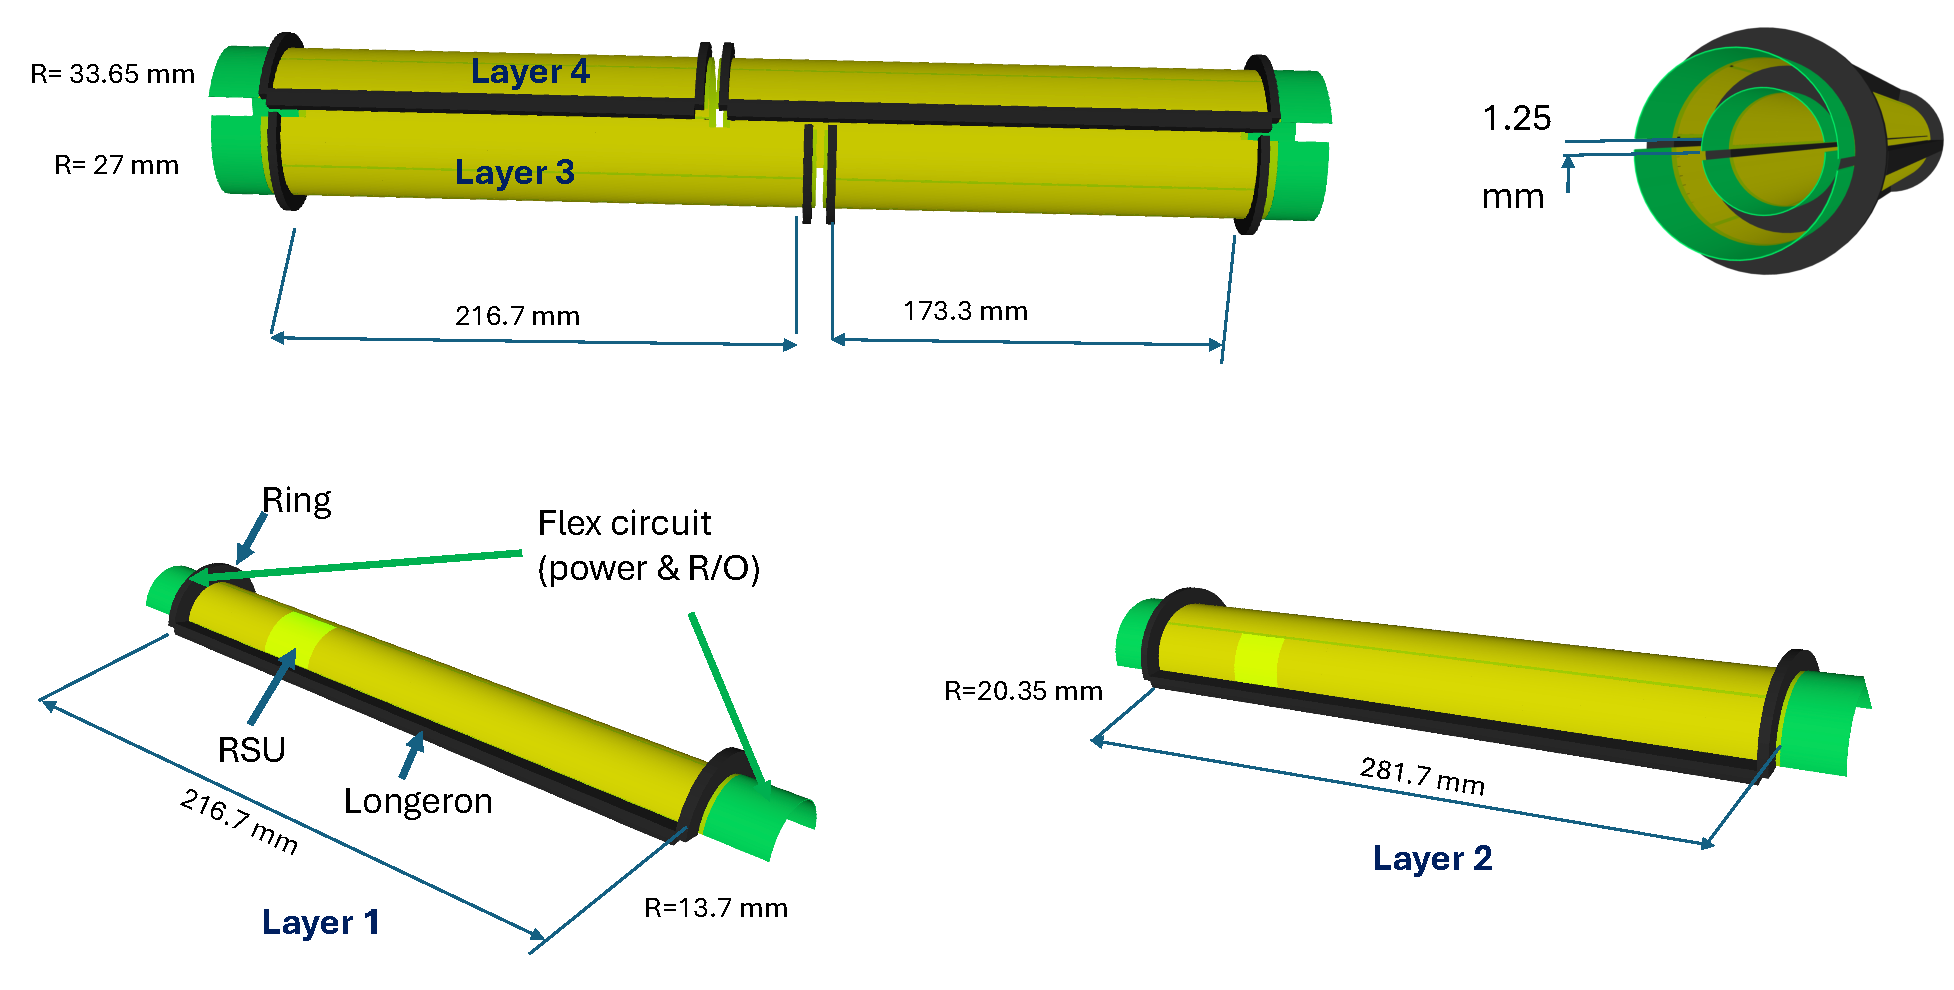
\includegraphics[width=0.95\linewidth]{Physics/DetectorConcepts/Figs/Vertex_curved.pdf}
\caption{Ultra-light inner vertex detector layout for the IDEA and ALLEGRO detector concepts. 
The four half-layers are shown separately in the top-left and in the bottom. 
The arrangement of the first two layers is shown in the top-right view.}
\label{fig:curved_vertex}
\end{figure}
\begin{figure}[ht]
\centering
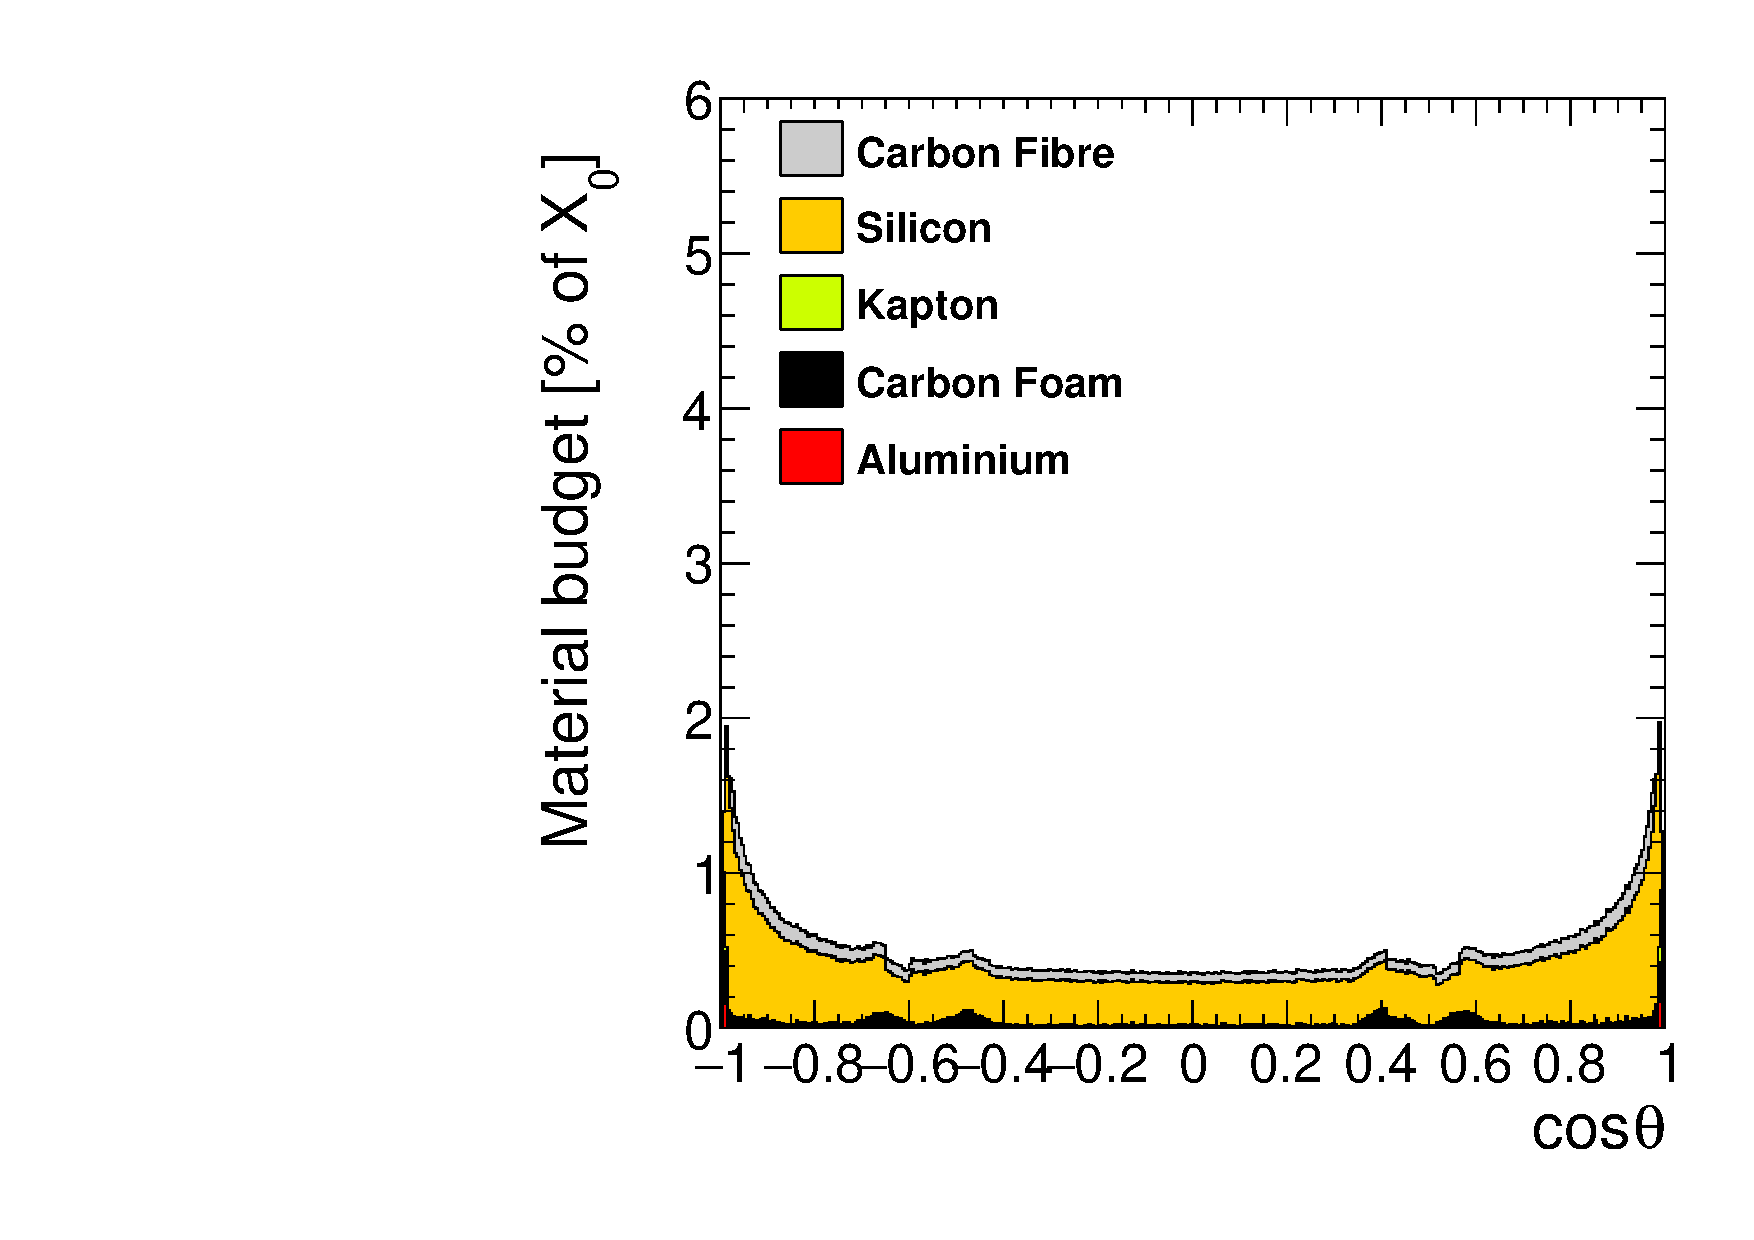
\includegraphics[width=0.46\textwidth]{Physics/DetectorConcepts/Figs/inner-vertex-ultralight-x0-1D.pdf}
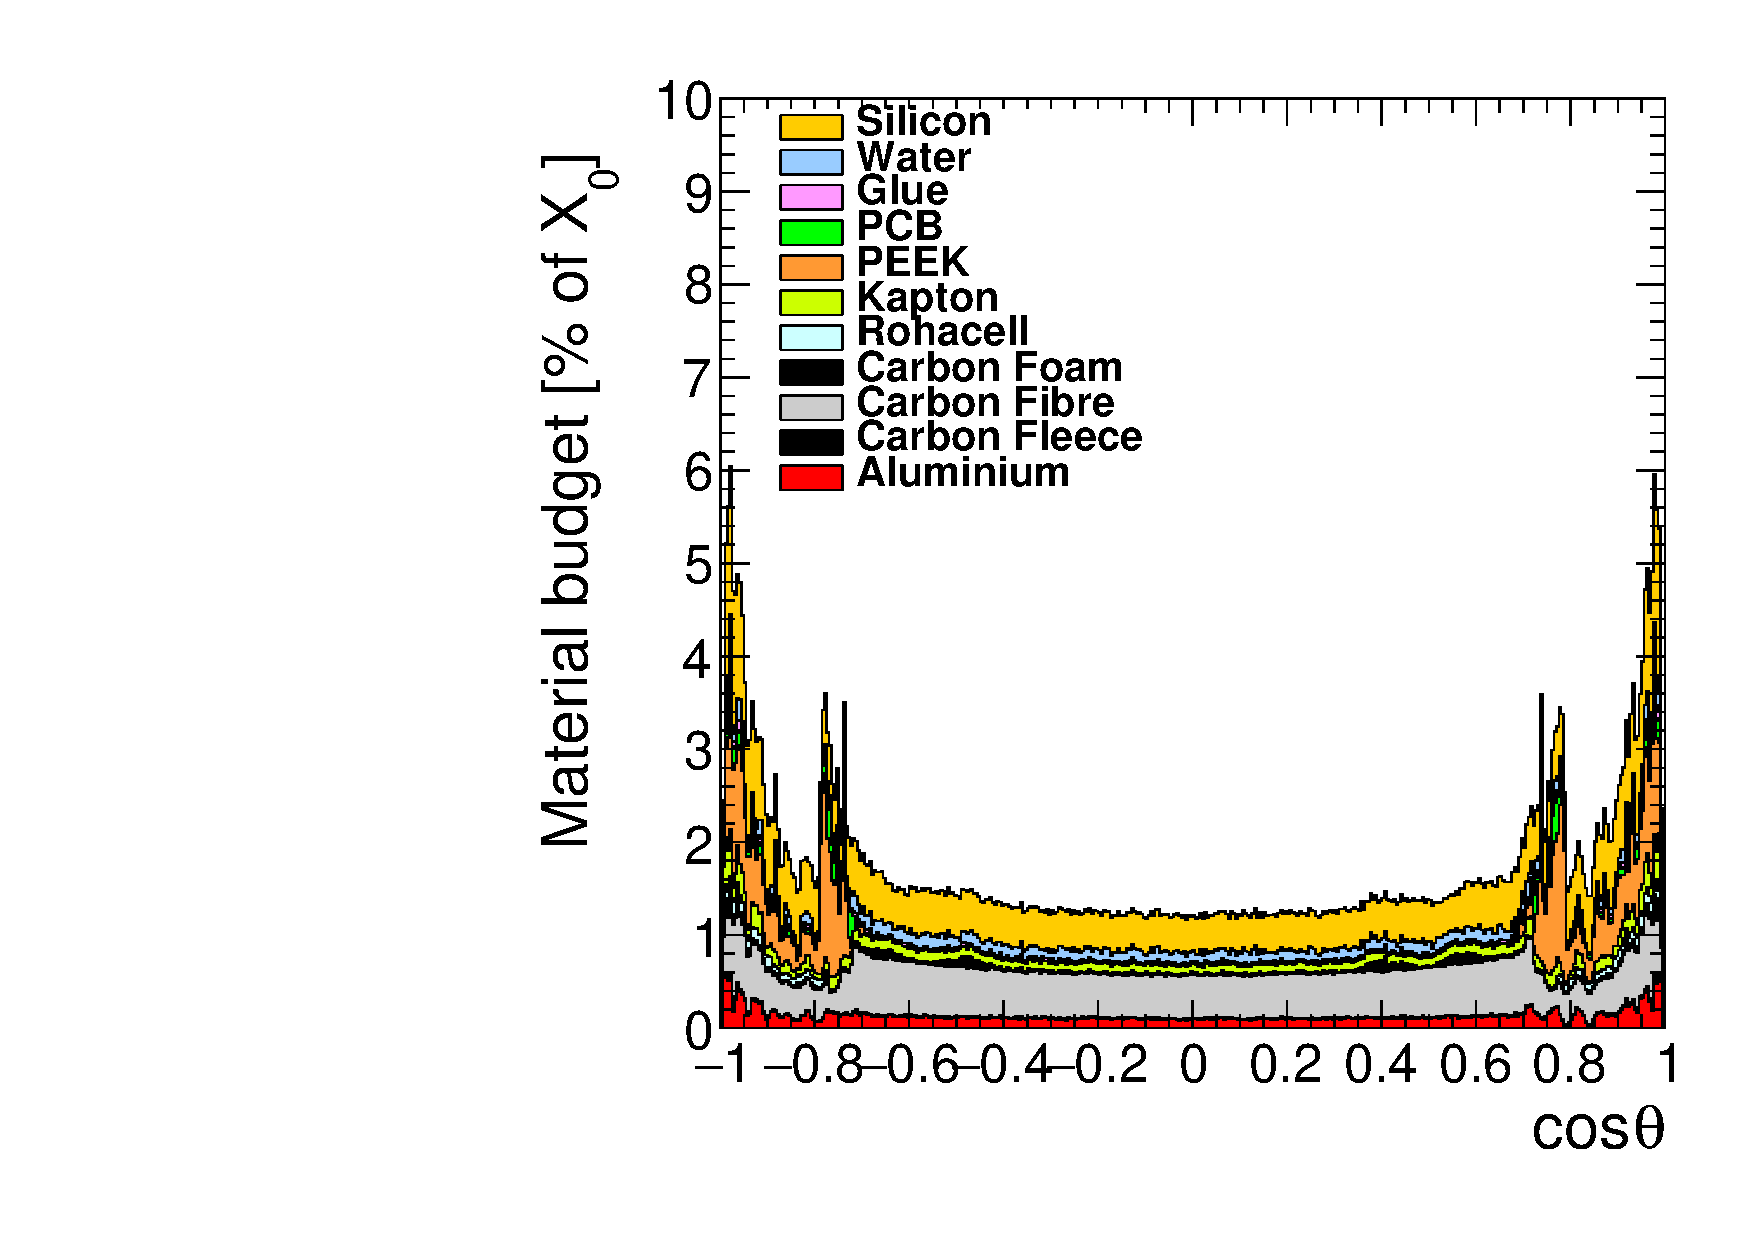
\includegraphics[width=0.46\textwidth]{Physics/DetectorConcepts/Figs/complete-vertex-ultrallight-x0-1D.pdf}
\caption{Material budget (expressed as a percentage of a radiation length) 
for the silicon vertex detectors considered for ALLEGRO and IDEA, 
for the inner vertex detector (left) 
and for the complete vertex detector in the ultra-light design (right), 
as a function of the cosine of the polar angle.}
\label{fig:UL_vtx_material_budget}
\end{figure}

A single layer contributes only about 0.07\%\,$X_0$, a reduction by about a factor three compared to the traditional design.
Furthermore, the material is more uniformly distributed in $\phi$, 
given the absence of overlapping structures in the same layer, 
as can be seen by comparing the left and right panels of Fig.~\ref{fig:vtx_material_budget_2D}.

\begin{figure}[ht]
\centering
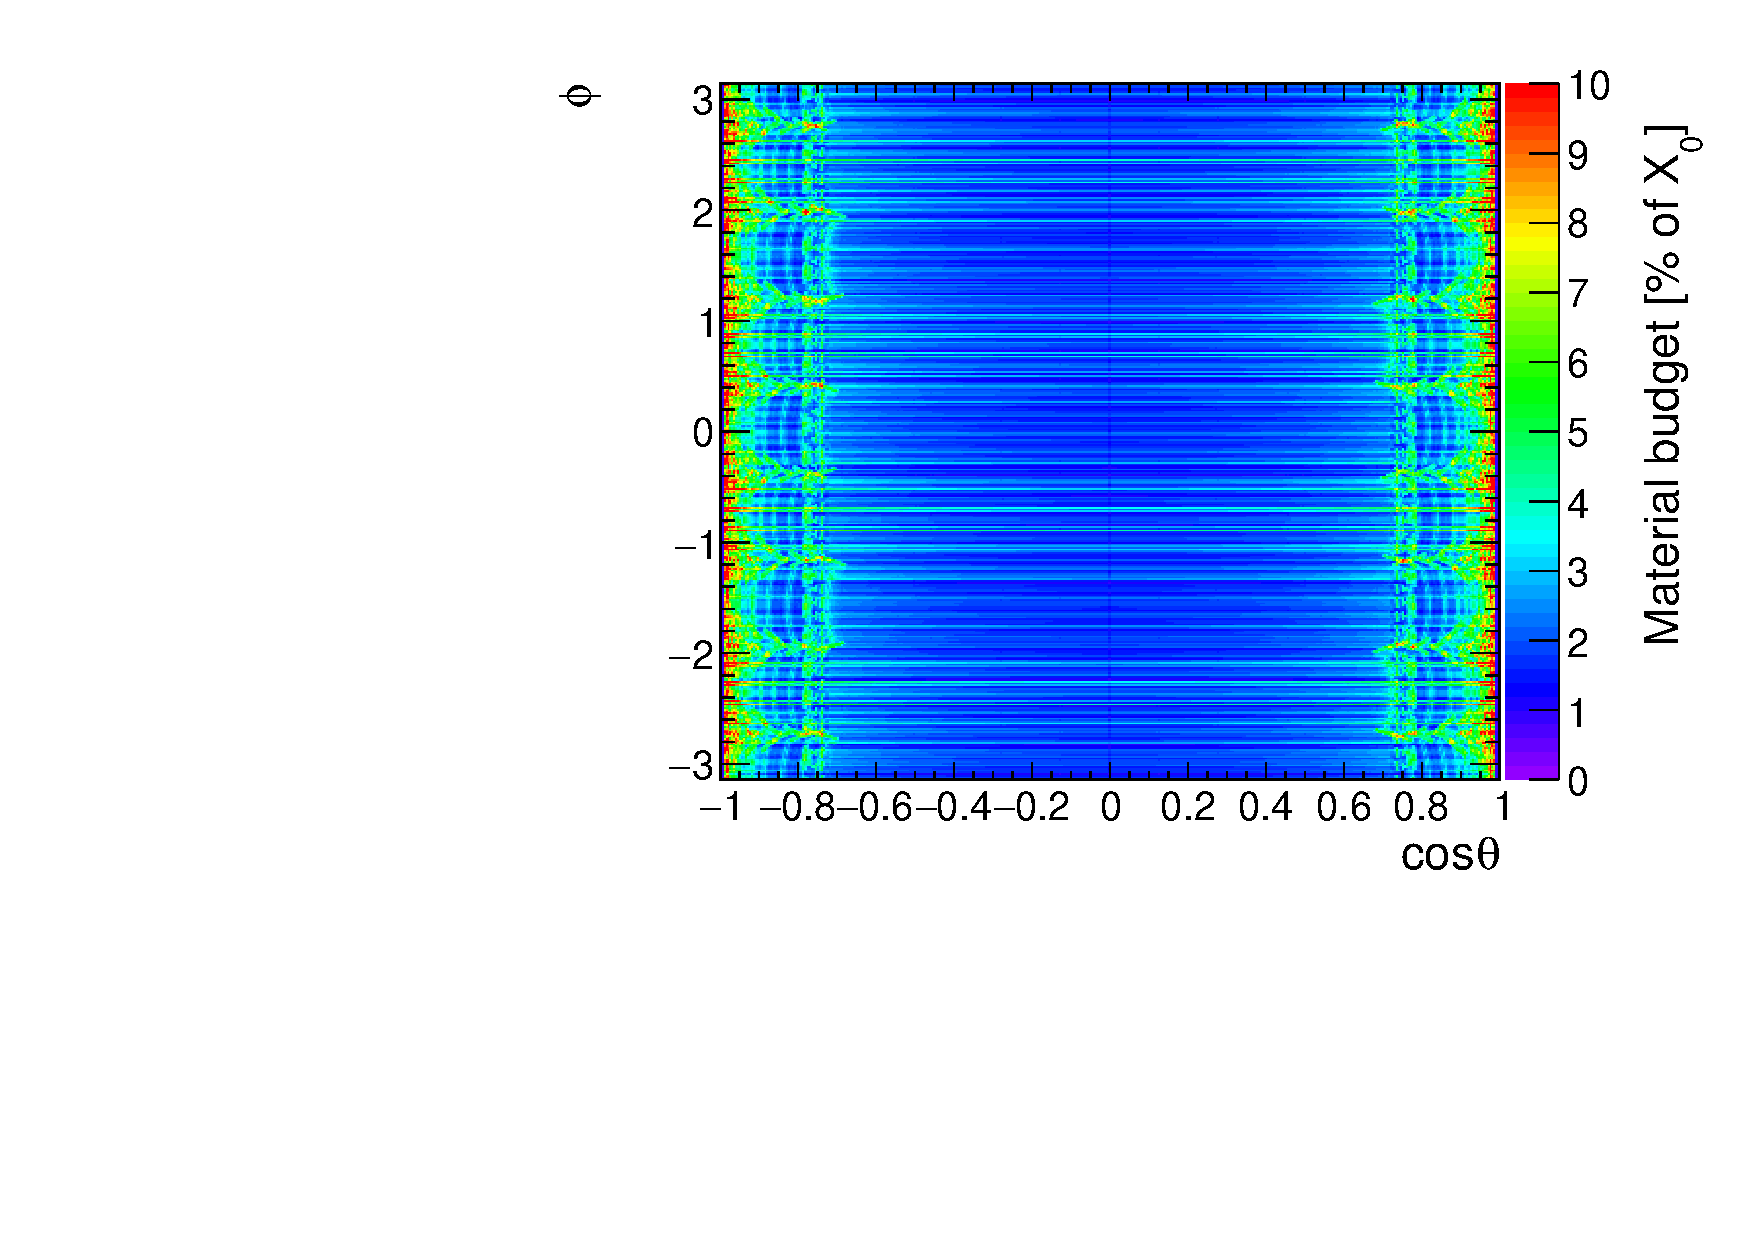
\includegraphics[width=0.49\textwidth]{Physics/DetectorConcepts/Figs/Vertex_x0_2D_-1_to_1.pdf}
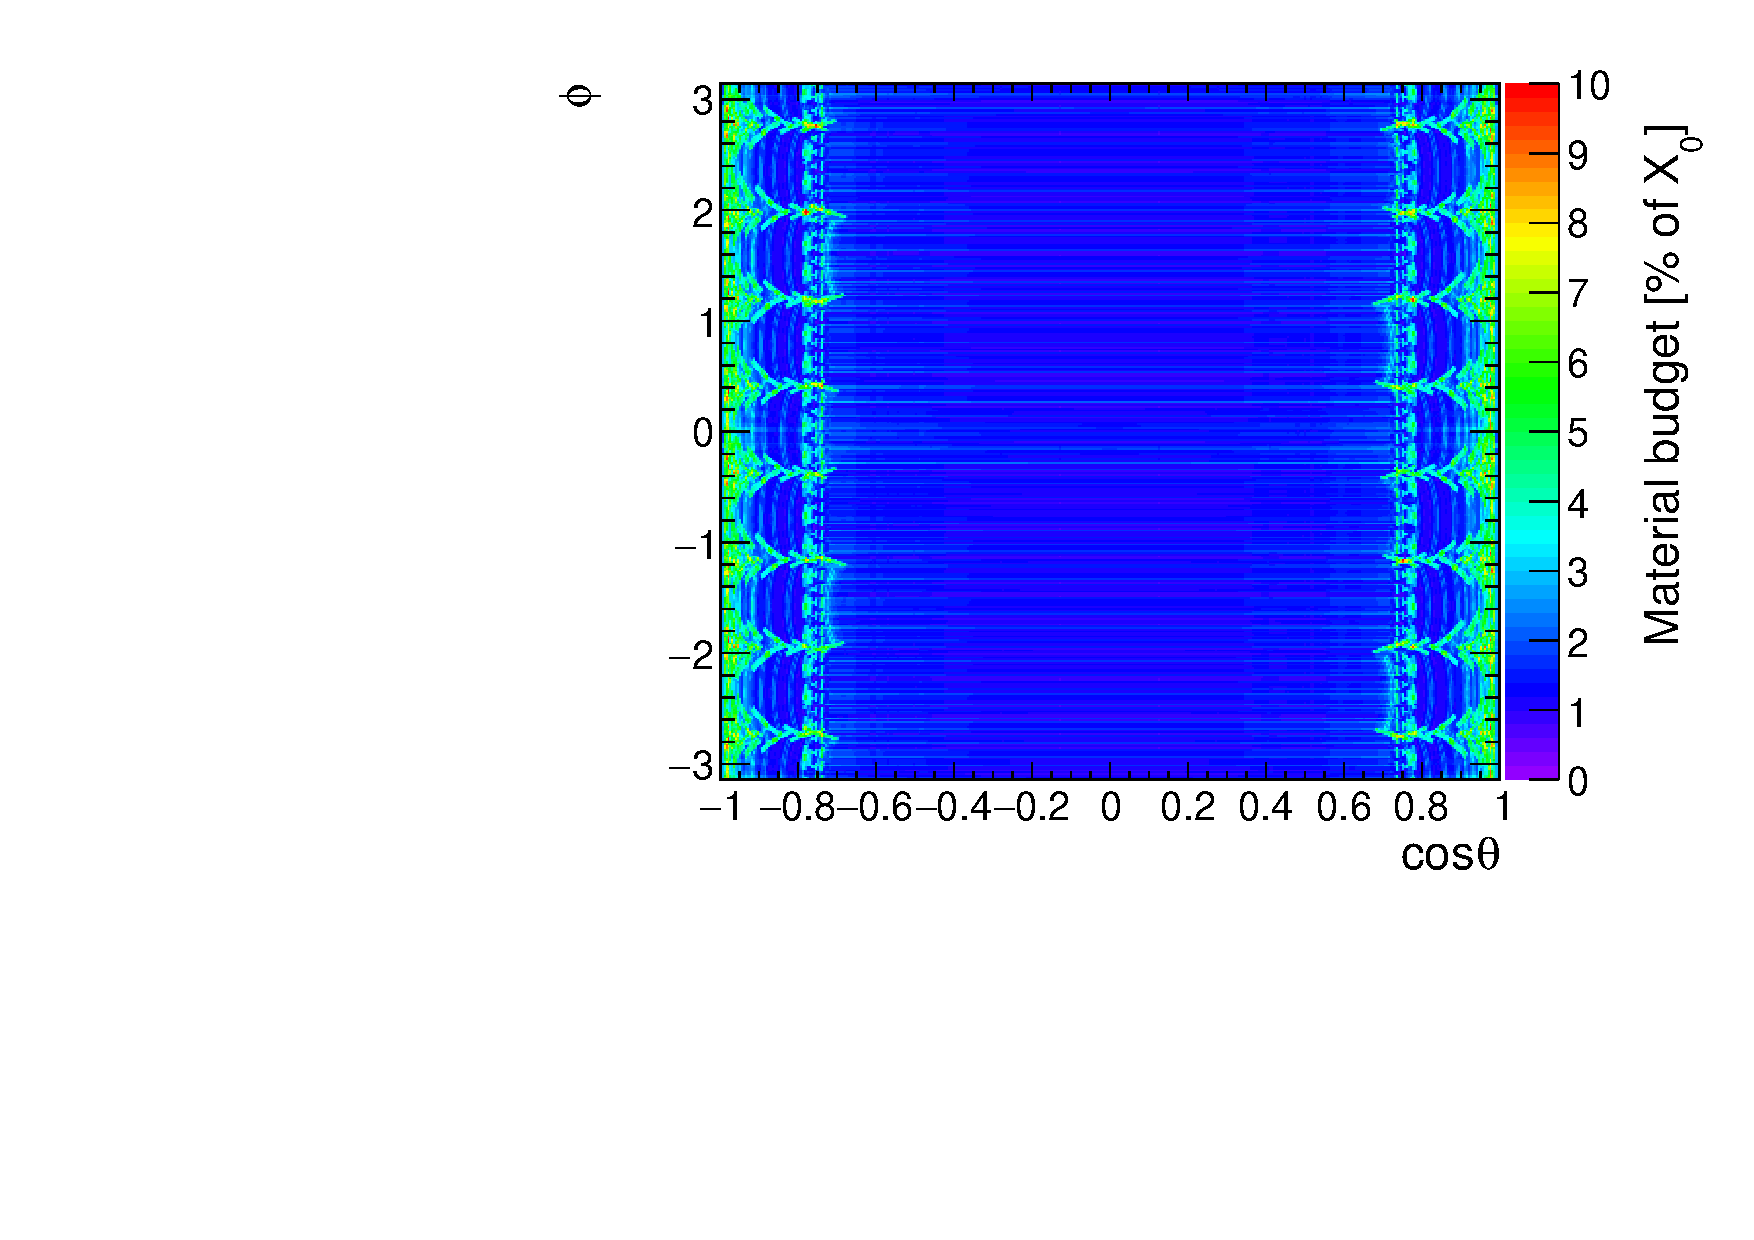
\includegraphics[width=0.49\textwidth]{Physics/DetectorConcepts/Figs/complete-vertex-ultralight-x0-2D.pdf}
\caption{Material budget (expressed as a percentage of a radiation length) 
for the silicon vertex detectors considered for ALLEGRO and IDEA in the baseline (left) and the ultra-light designs (right), 
for the complete vertex detector, as a function of the azimuthal angle vs.\ the cosine of the polar angle.}
\label{fig:vtx_material_budget_2D}
\end{figure}

For both alternatives, the outer vertex detector is composed of two barrel layers and three disks on each side. 
The elementary unit is a module of area $40.6\,(z) \times 42.2\,(r\phi)$\,mm$^2$. 
Each module has four hybrid pixel sensor chips, inspired by the ATLASPIX3 R\&D~\cite{ATLASPIX3}. 
The 50\,$\mu$m thick sensor has $372 \times 132$ pixels of $50 \times 150$\,$\mu$m$^2$ area. 
The power consumption is assumed to be 100\,mW/cm$^2$, 
half of the level observed at the current stage of development, 
but still too high (by at least a factor of two) to be handled by air cooling.
The modules are placed on a lightweight triangular truss structure. 
The staves are mechanical structures that hold the modules.
A stave is composed of a carbon-fibre multilayered structure, 
consisting of 120\,$\mu$m thick carbon fibre KDU13 and two carbon fleeces of 65\,$\mu$m in total, 
to support two 90\,$\mu$m thick polymide tubes of 2.2\,mm diameter, where demineralised cooling water circulates. 
An electronic bus, providing power distribution and readout and control signals, 
runs along the entire stave length and is placed on top of the modules. 
It is terminated, at the end of both sides, by a hybrid circuit.

The middle barrel layer is positioned at a radius of 130\,mm and is composed of 22 ladders, each with 8 modules.
The outer barrel layer is placed at a radius of 315\,mm and is composed of 51 ladders, of 16 modules each.
The outer and middle barrels are supported by a flange attached to an external support tube. 
The flange also supports the two innermost disks.
%
Three disks per side, located at $|z|$ = 304.7, 620, and 930\,mm, complete the outer vertex tracker. 
The inner disk is located inside the barrel.
Each disk is composed of eight petals, 
four facing the IP and four facing the opposite direction,
made of modules of the same type as those of the barrels.
The support structure of each disk is made of a sandwich of thin carbon fibre walls (each 0.3\,mm thick) 
interleaved with 5.4\,mm thick Rohacell~\cite{Rohacell}. 
The material budget of the outer vertex detector is about 1\% of a radiation length at normal incidence, 
increasing to about 3\% at the edges of the middle and outer barrel, because of the supports and hybrid circuits.

The vertex detector of the CLD concept~\cite{Bacchetta:2019fmz}, composed of a cylindrical barrel and forward disks, 
is located at radii below 112\,mm. 
The layout is based on double layers of ultralight MAPS fixed on a common support structure that includes cooling circuits. 
The 125\,mm long barrel comprises three double layers (0.63\%\,$X_0$ each) at radii 12.5--13.5, 37--38, and 57--58\,mm. 
Three disks on each side (0.70\%\,$X_0$ each), at distances from the IP of 160, 230, and 300\,mm, complete the detector. 
For simulation studies, a point resolution of $3 \times 3$\,$\mu$m$^2$ is assumed.

Full simulation studies~\cite{Sadowski:2024} with the smaller radius beam pipe 
introduced since the publication of Ref.~\cite{Bacchetta:2019fmz} 
(the inner radius decreased from 15 to 10\,mm)
and a corresponding reduction of the radius of the inner barrel layer 
confirm earlier conclusions from fast simulations~\cite{Bacchetta:2019fmz} 
of a better impact parameter resolution and a significantly improved flavour-tagging performance. 
Even with a simultaneous increase of the beam-pipe material budget from 0.45\% to 0.61\%\,$X_0$, 
the studies show, for example, an impact parameter resolution improved by 20\% for 10\,GeV tracks.

\subsection{Main tracking systems}
\label{sec:Detectors_MainTracking}

\subsubsection{Silicon tracker}

The CLD concept features an all-silicon tracker,
complementing the vertex detector (briefly described at the end of the previous section) 
with a `main tracker', itself divided into inner and outer sections 
by a lightweight (1.25\%\,$X_0$) carbon-fibre support tube, at a radius of 690\,mm.
The inner tracker comprises three barrel layers and seven forward disks on each end-cap,
while the outer tracker has three more barrel layers and four disks on each side. 
The material budget of the modules 
(200\,$\mu$m of silicon sensors, or 0.21\%\,$X_0$, including electronics),
plus cooling and connectivity, 
is estimated to range between 1.1\% and 1.3\%\,$X_0$. 
In addition, carbon-fibre support structures, which differ from layer to layer, 
contribute between 0.13\% and 0.37\%\,$X_0$.
For simulation studies, 
point resolutions of $5 \times 5$\,$\mu$m$^2$ and $7 \times 90$\,$\mu$m$^2$
are assumed for the innermost disk of the inner tracker and for all other layers, respectively.
The material budget of the complete CLD tracking system,
including the vertex detector and the main tracker (plus the beam pipe),
is shown in Fig.~\ref{fig:CLD:TrackerMaterialBudget}.

\begin{figure}[ht]
\centering
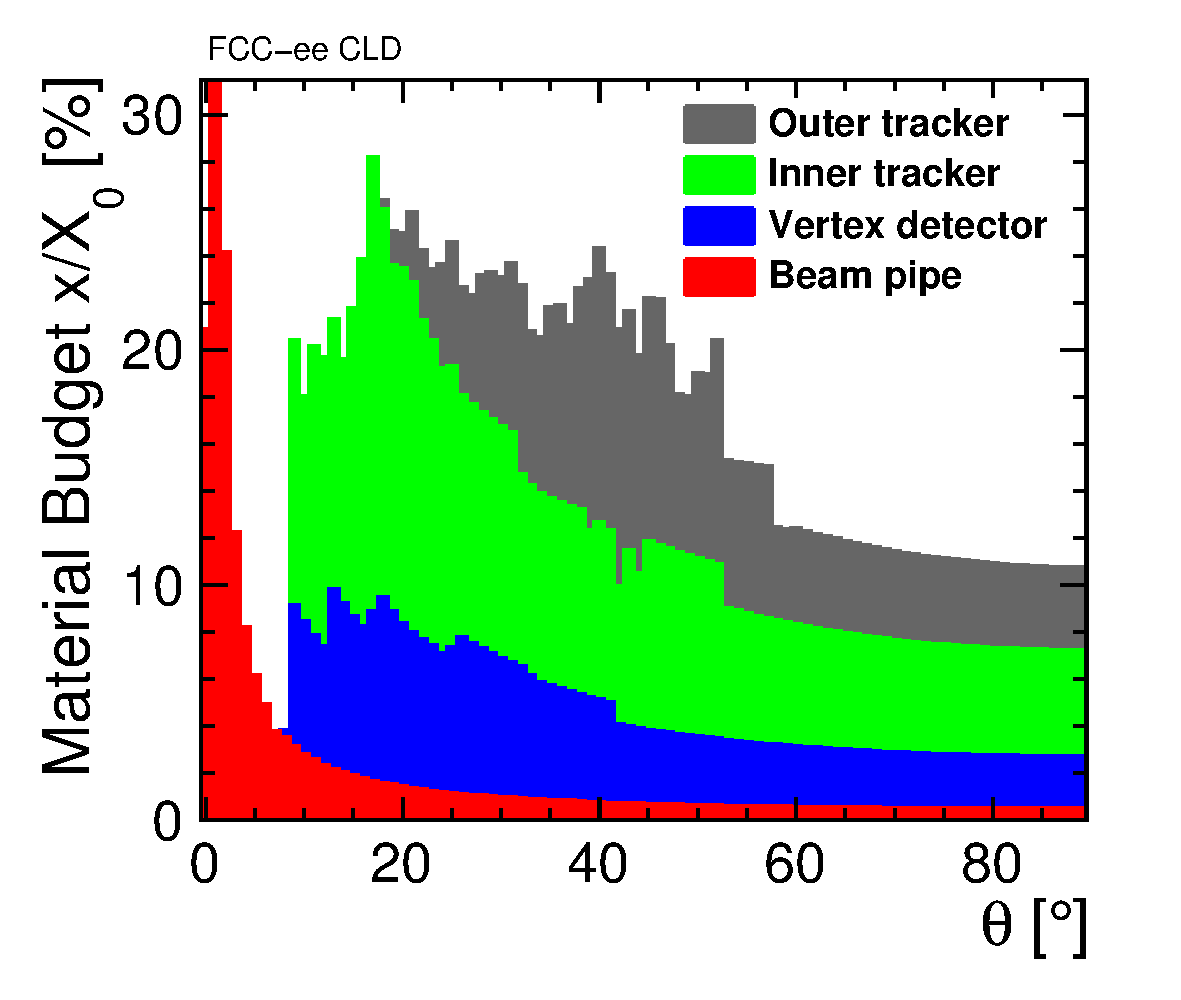
\includegraphics[width=0.60\textwidth]{Physics/DetectorConcepts/Figs/materialBudget_FCCee_o1_v04.pdf}
\caption{Stacked material budget (expressed as a percentage of a radiation length) 
of the different parts of the CLD tracking system (plus the beam pipe), 
as a function of the polar angle and averaged over the azimuthal angle, 
including contributions from sensitive layers, cables, supports, and cooling.}
\label{fig:CLD:TrackerMaterialBudget}
\end{figure}

Full-simulation studies to assess the performance of the CLD tracker are reported in Ref.~\cite{Bacchetta:2019fmz}. 
Figure~\ref{fig:CLD:resolutions} shows some essential performance figures for single muons: 
the momentum and impact parameter resolutions, 
as well as the polar and azimuthal angular resolutions. 
For $\pt > 100$\,GeV, the momentum resolution curves start to flatten out, 
reaching an asymptotic value of $\delta (1/\pt) \simeq 1 \times 10^{-5}$\,GeV$^{-1}$. 
For lower momenta, the momentum resolution is dominated by multiple scattering.
More studies are needed to further reduce the material budget, 
in particular for the support structures and services.

\begin{figure}[ht]
\centering
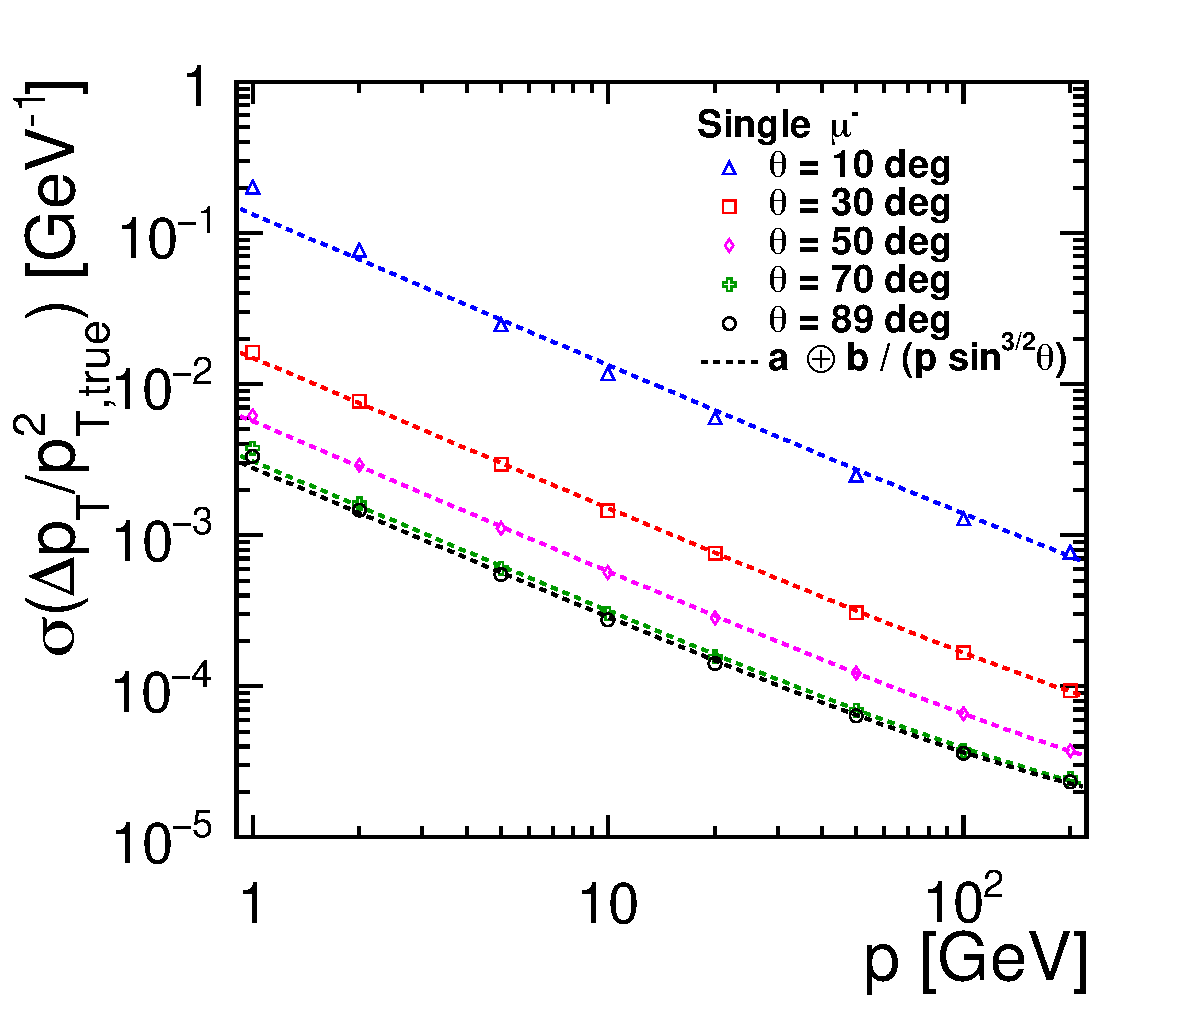
\includegraphics[width=0.49\textwidth]{Physics/DetectorConcepts/Figs/MomRes_vs_p-4.pdf}
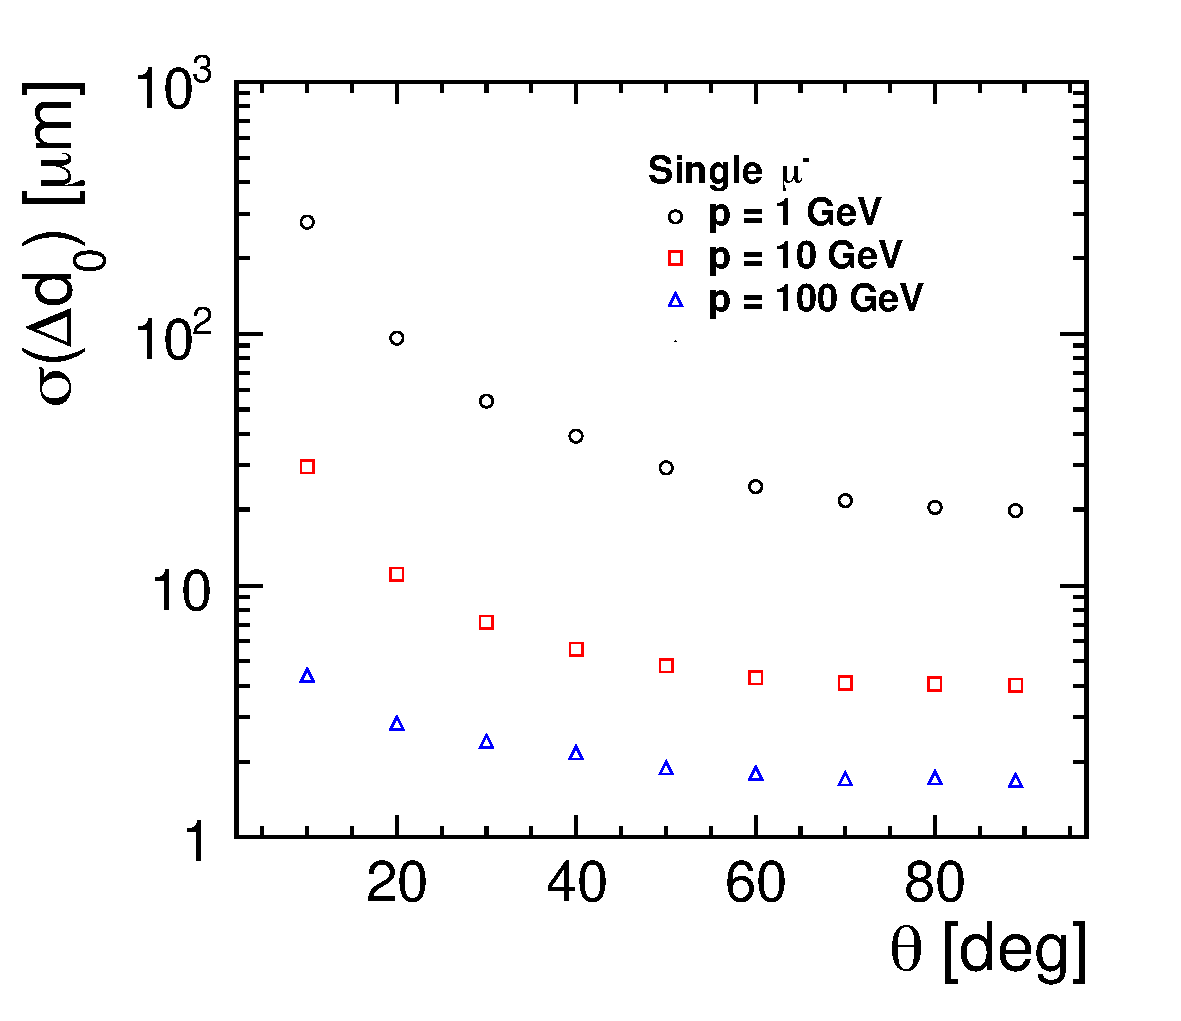
\includegraphics[width=0.49\textwidth]{Physics/DetectorConcepts/Figs/d0Res_vs_theta-1b.pdf}
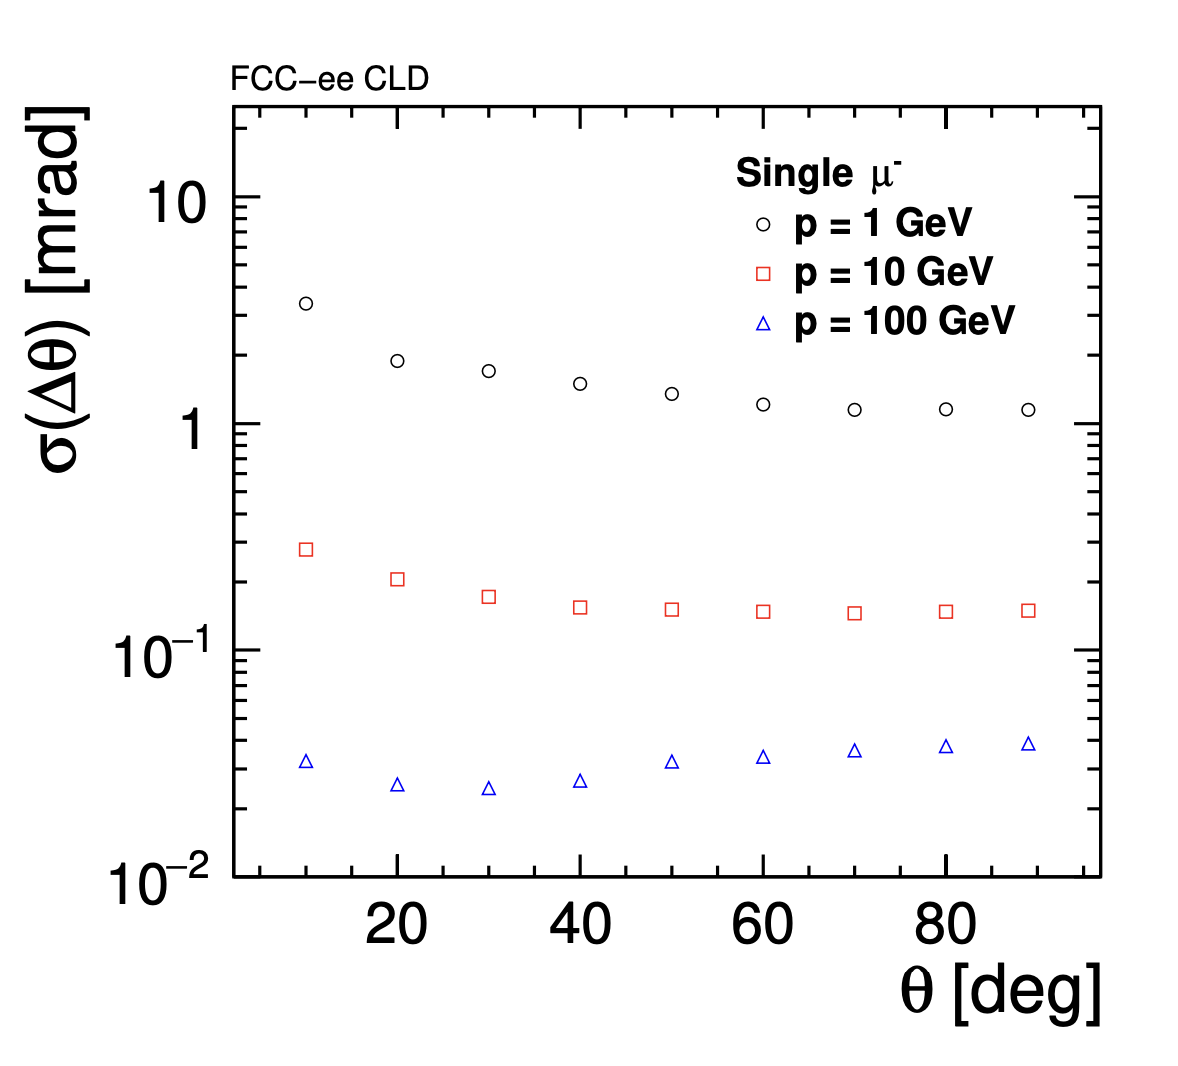
\includegraphics[width=0.49\textwidth]{Physics/DetectorConcepts/Figs/CLD_thetaRes.png}
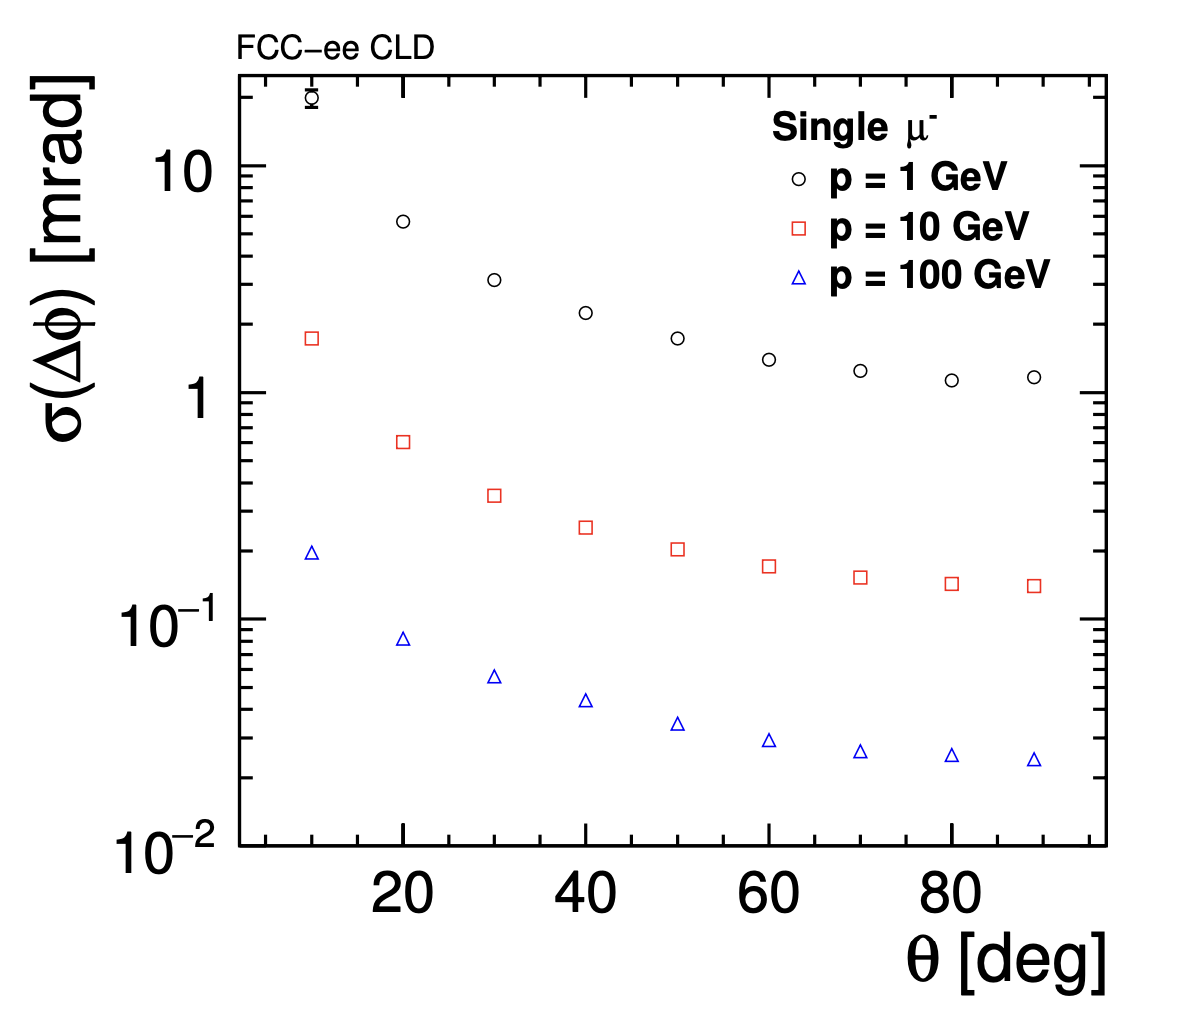
\includegraphics[width=0.49\textwidth]{Physics/DetectorConcepts/Figs/CLD_phiRes.png}
\caption{Top-left: Transverse momentum resolution for single muons as a function of momentum at five fixed polar angle values.
Polar-angle dependence of the impact parameter resolution in the transverse plane (top-right), 
of the polar angle resolution (bottom-left), 
and of the azimuthal angle resolutions (bottom-right), 
for muon momenta of 1, 10, and 100\,GeV.
From Ref.~\cite{Bacchetta:2019fmz}.}
\label{fig:CLD:resolutions}
\end{figure}

A smaller tracker outer radius would, in particular, allow for the insertion of a compact RICH detector, 
such as the ARC detector (Section~\ref{sec:ARC}), 
which could provide improved particle identification performance at the cost of a worse momentum resolution. 
A recent full-simulation study~\cite{Sadowski:2024} confirms fast-simulation indications 
that a reduction of the tracker outer radius from 2.31 to 1.80\,m leads to a degradation of the momentum resolution by about 15\%, 
showing that the momentum resolution scales roughly like $1/R$, where $R$ is the outer tracker radius. 
This observation is compatible with expectations in cases where multiple scattering is the dominant effect
(otherwise, a $1/R^2$ dependence would be expected). 
The study also confirms that an increase of the magnetic field strength from 2 to 3\,T 
would lead to a $\sim$\,30\% improvement of the \pt resolution. 

\subsubsection{Drift chamber}

The IDEA concept features the InTrEPId (Inner Tracking Equipped with Particle Identification) drift chamber, 
designed to provide tracking with high-precision momentum measurement and particle identification by cluster counting. 
A high transparency is obtained by a novel approach for the wiring and assembly procedures~\cite{chiarello}. 
The total amount of material is about 1.6\%\,$X_0$ at normal incidence (dominated by the outer container material), 
increasing to about 5.0\%\,$X_0$ in the forward direction 
(the end plates instrumented with front-end electronics contributing 75\% of that value). 
The drift chamber is a single-volume, high-granularity, all-stereo, short-drift, low-mass cylindrical wire chamber, 
co-axial with the 2\,T magnetic field. 
It extends from an inner radius of 0.35\,m to an outer radius of 2\,m, has a length of 4\,m along the $z$ axis, 
and consists of 112 co-axial layers, at alternating-sign stereo angles, arranged in 24 identical azimuthal sectors. 
The angular coverage extends down to $\sim$\,13$^\circ$ (227\,mrad). 
The size of the approximately square cells ranges between 12 and 14.5\,mm, for a total of 56\,448 drift cells.
The challenges potentially arising from a large number of wires (about 350\,000 in total) 
are addressed by the design of the wiring procedures, 
successfully exploited during the recent construction of the MEG2 drift chamber~\cite{chiappini2}. 

A very light gas mixture, 90\%~He and 10\%~iC$_4$H$_{10}$, corresponding to a maximum drift time of $\sim$\,400\,ns, 
is expected to be used in operation. 
The number of ionisation clusters generated by a minimum ionising particle is about 12.5\,cm$^{-1}$, 
allowing cluster counting/timing techniques to be exploited,
to improve both the spatial resolution (better than 100\,$\mu$m)
and the particle identification resolution ($\sim$\,3\%).
A spatial resolution around 120\,$\mu$m has been achieved in the 7\,mm cell size MEG2 drift chamber 
with the same gas mixture and very similar electrostatic configuration~\cite{afanaciev}. 
An even better spatial resolution is expected in InTrEPId, 
with the application of cluster timing techniques on the one hand and with the longer drift on the other, 
which mitigates, on average, the effects of the short-drift stochastic behaviour.

Fast simulation studies have been performed with \textsc{Delphes} to evaluate the tracking performance, 
with the vertex detector, the drift chamber, and a surrounding double layer of silicon microstrip detectors. 
This `Si wrapper' provides an additional accurate space point with an assumed resolution of $7 (r\phi) \times 90 (z)$\,$\mu$m$^2$, 
and a precise definition of the tracker acceptance. 
Details of ionisation clustering to exploit the cluster counting/timing technique were not simulated, 
conservatively limiting the spatial resolution of the drift chamber to 100\,$\mu$m. 
The resulting momentum resolution is displayed in Fig.~\ref{fig:dch1}. 
For transverse momenta in excess of $\sim$\,20\,GeV, 
the resolution is well described by $\delta \pt / \pt^2 = 3 \times 10^{-5}$\,GeV$^{-1}$.
Angular resolutions better than 0.1\,mrad are obtained in both the azimuthal and polar angles. 

\begin{figure}[ht]
\centering
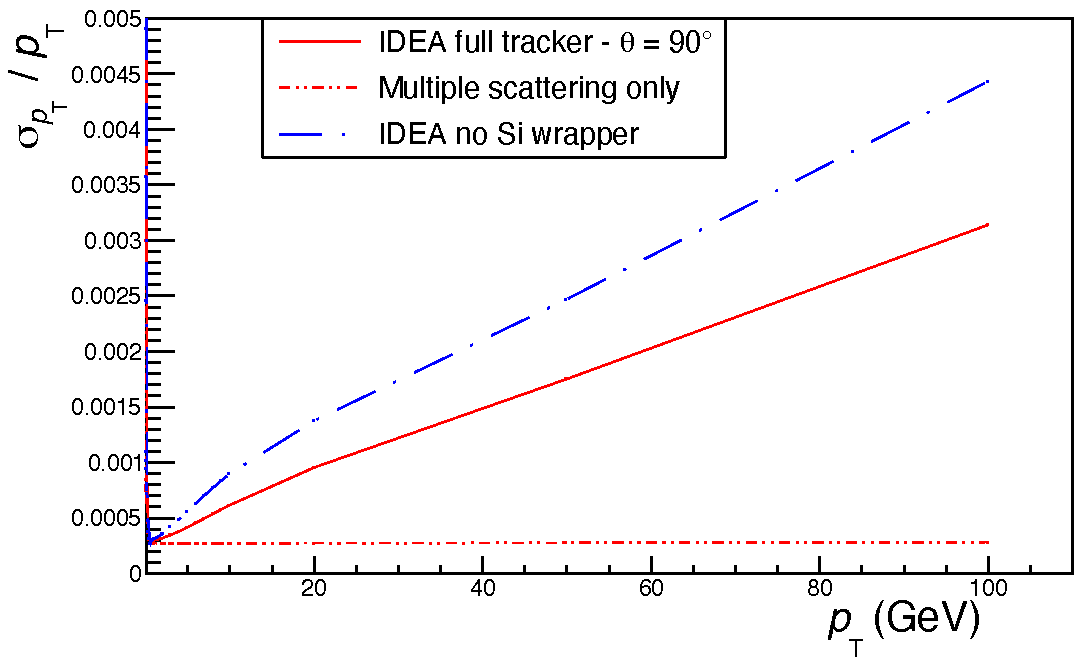
\includegraphics[width=0.5\linewidth]{Physics/DetectorConcepts/Figs/IDEAresPlot-CL.pdf}
\caption{Transverse momentum resolution as a function of \pt, for tracks at a polar angle of 90$^\circ$,
in the IDEA tracking system (full red curve). 
The contributions from multiple scattering (dot-dashed red curve) and the impact of the silicon wrapper (dash-dotted blue curve) are also illustrated.}
\label{fig:dch1}
\end{figure}

Cluster counting and timing provide a $\PGp/\PK$ separation better than three standard deviations up to momenta about 30\,GeV, 
except in a narrow gap between 0.9 and 1.6\,GeV, where the Bethe--Bloch energy-loss curves for the two particle types cross. 
These values were obtained with a fast simulation study that parametrised \textsc{Garfield++}~\cite{garfield} results within \textsc{Delphes}. 
As illustrated in Fig.~\ref{fig:dch4}, the gap can be adequately covered with a time-of-flight measurement over a distance of 2\,m, 
with a non-challenging resolution of $\mathcal{O}(100)$\,ps.

\begin{figure}[ht]
\centering
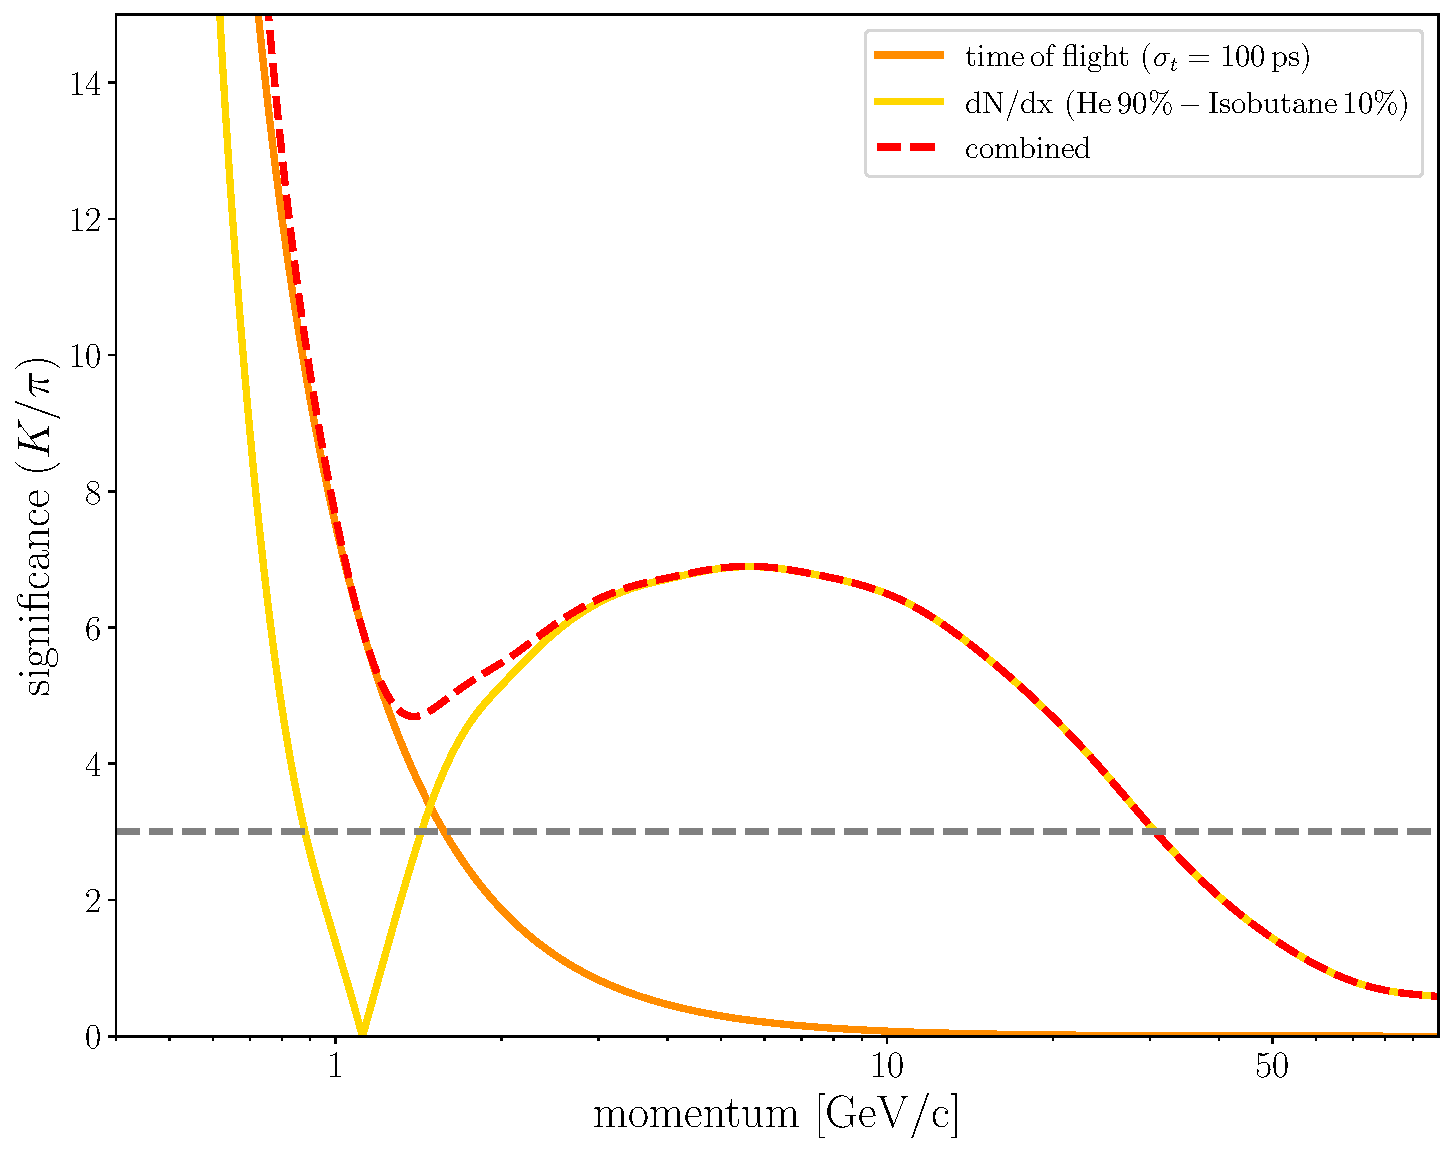
\includegraphics[width=0.55\linewidth]{Physics/DetectorConcepts/Figs/combined_pid.pdf}
\caption{Significance (in standard deviations) of the $\PGp/\PK$ separation in the IDEA drift chamber, 
from a fast \textsc{Delphes} simulation study, 
with the cluster counting performance parametrised from \textsc{Garfield++} results (yellow curve).
A better than 3\,$\sigma$ separation is obtained up to momenta $\sim$\,30\,GeV. 
The $p < 1.6$\,GeV region is covered by a time-of-flight system, 
extending over a distance of 2\,m and with a timing resolution assumed to be 100\,ps (orange curve). 
The combination of the drift chamber and the time-of-flight system is represented by the dashed red curve.}
\label{fig:dch4}
\end{figure}

\subsubsection{Straw tracker}

A straw tracker with thin Mylar walls may also be a promising option to meet the stringent FCC-ee detector requirements,
when combined with a pixel detector near the beam pipe and a silicon wrapper as an outer layer. 
A straw tracker can provide a spatial resolution of 100--120\,$\mu$m per straw 
and a low material budget of 1.2\%\,$X_0$ at $\theta = 90^{\circ}$ for 100 layers of straws 
made with 12\,$\mu$m-thick Mylar walls. 
With ${\cal{O}}(100)$ hits per track, 
such a straw tracker is well suited for both pattern recognition and searches for long-lived particles. 
In addition, it can provide excellent particle identification capabilities, 
such as $\PGp/\PK$ and $\PK/\Pp$ discrimination, 
across a wide momentum range and could also be used for triggering purposes, 
making it valuable for both collider data taking and cosmic ray studies.

Each straw functions as an independent channel, providing significant flexibility for design optimisation. 
The operational robustness also benefits from the fact that each straw can be easily disconnected if its wire breaks. 
The electric charges generated within a straw remain confined to that specific unit. 
The electric field within a straw is radially symmetric, 
making the resolution independent of the particle incident angle and leading to a good single-hit resolution. 
Straws with different radii can be used in various detector regions to optimise hit occupancy, 
material budget, and channel counting. 
The gas mixture can be optimised to enhance particle identification capabilities 
and different gas mixtures can be simultaneously used for straws in different layers.

Figure~\ref{fig:straw_tracker} shows an example layout of a straw tracker implemented in a \textsc{Geant4} simulation, 
featuring ${\cal{O}}(60\,000)$ straws with a diameter of 1 to 1.5\,cm and a length of 5\,m,
arranged in ten concentric superlayers. 
Straws are arranged in both axial and stereo layers with a stereo angle of a few degrees 
to determine the hit position with an accuracy of a few mm along the $z$ direction. 
Initial simulations~\cite{StrawTrackerRnD} predict similar momentum resolutions as with the InTrEPId drift chamber. 

\begin{figure}[t]
\centering
\includegraphics[width=0.54\linewidth]{Physics/DetectorConcepts/Figs/StrawTracker-layout.pdf}
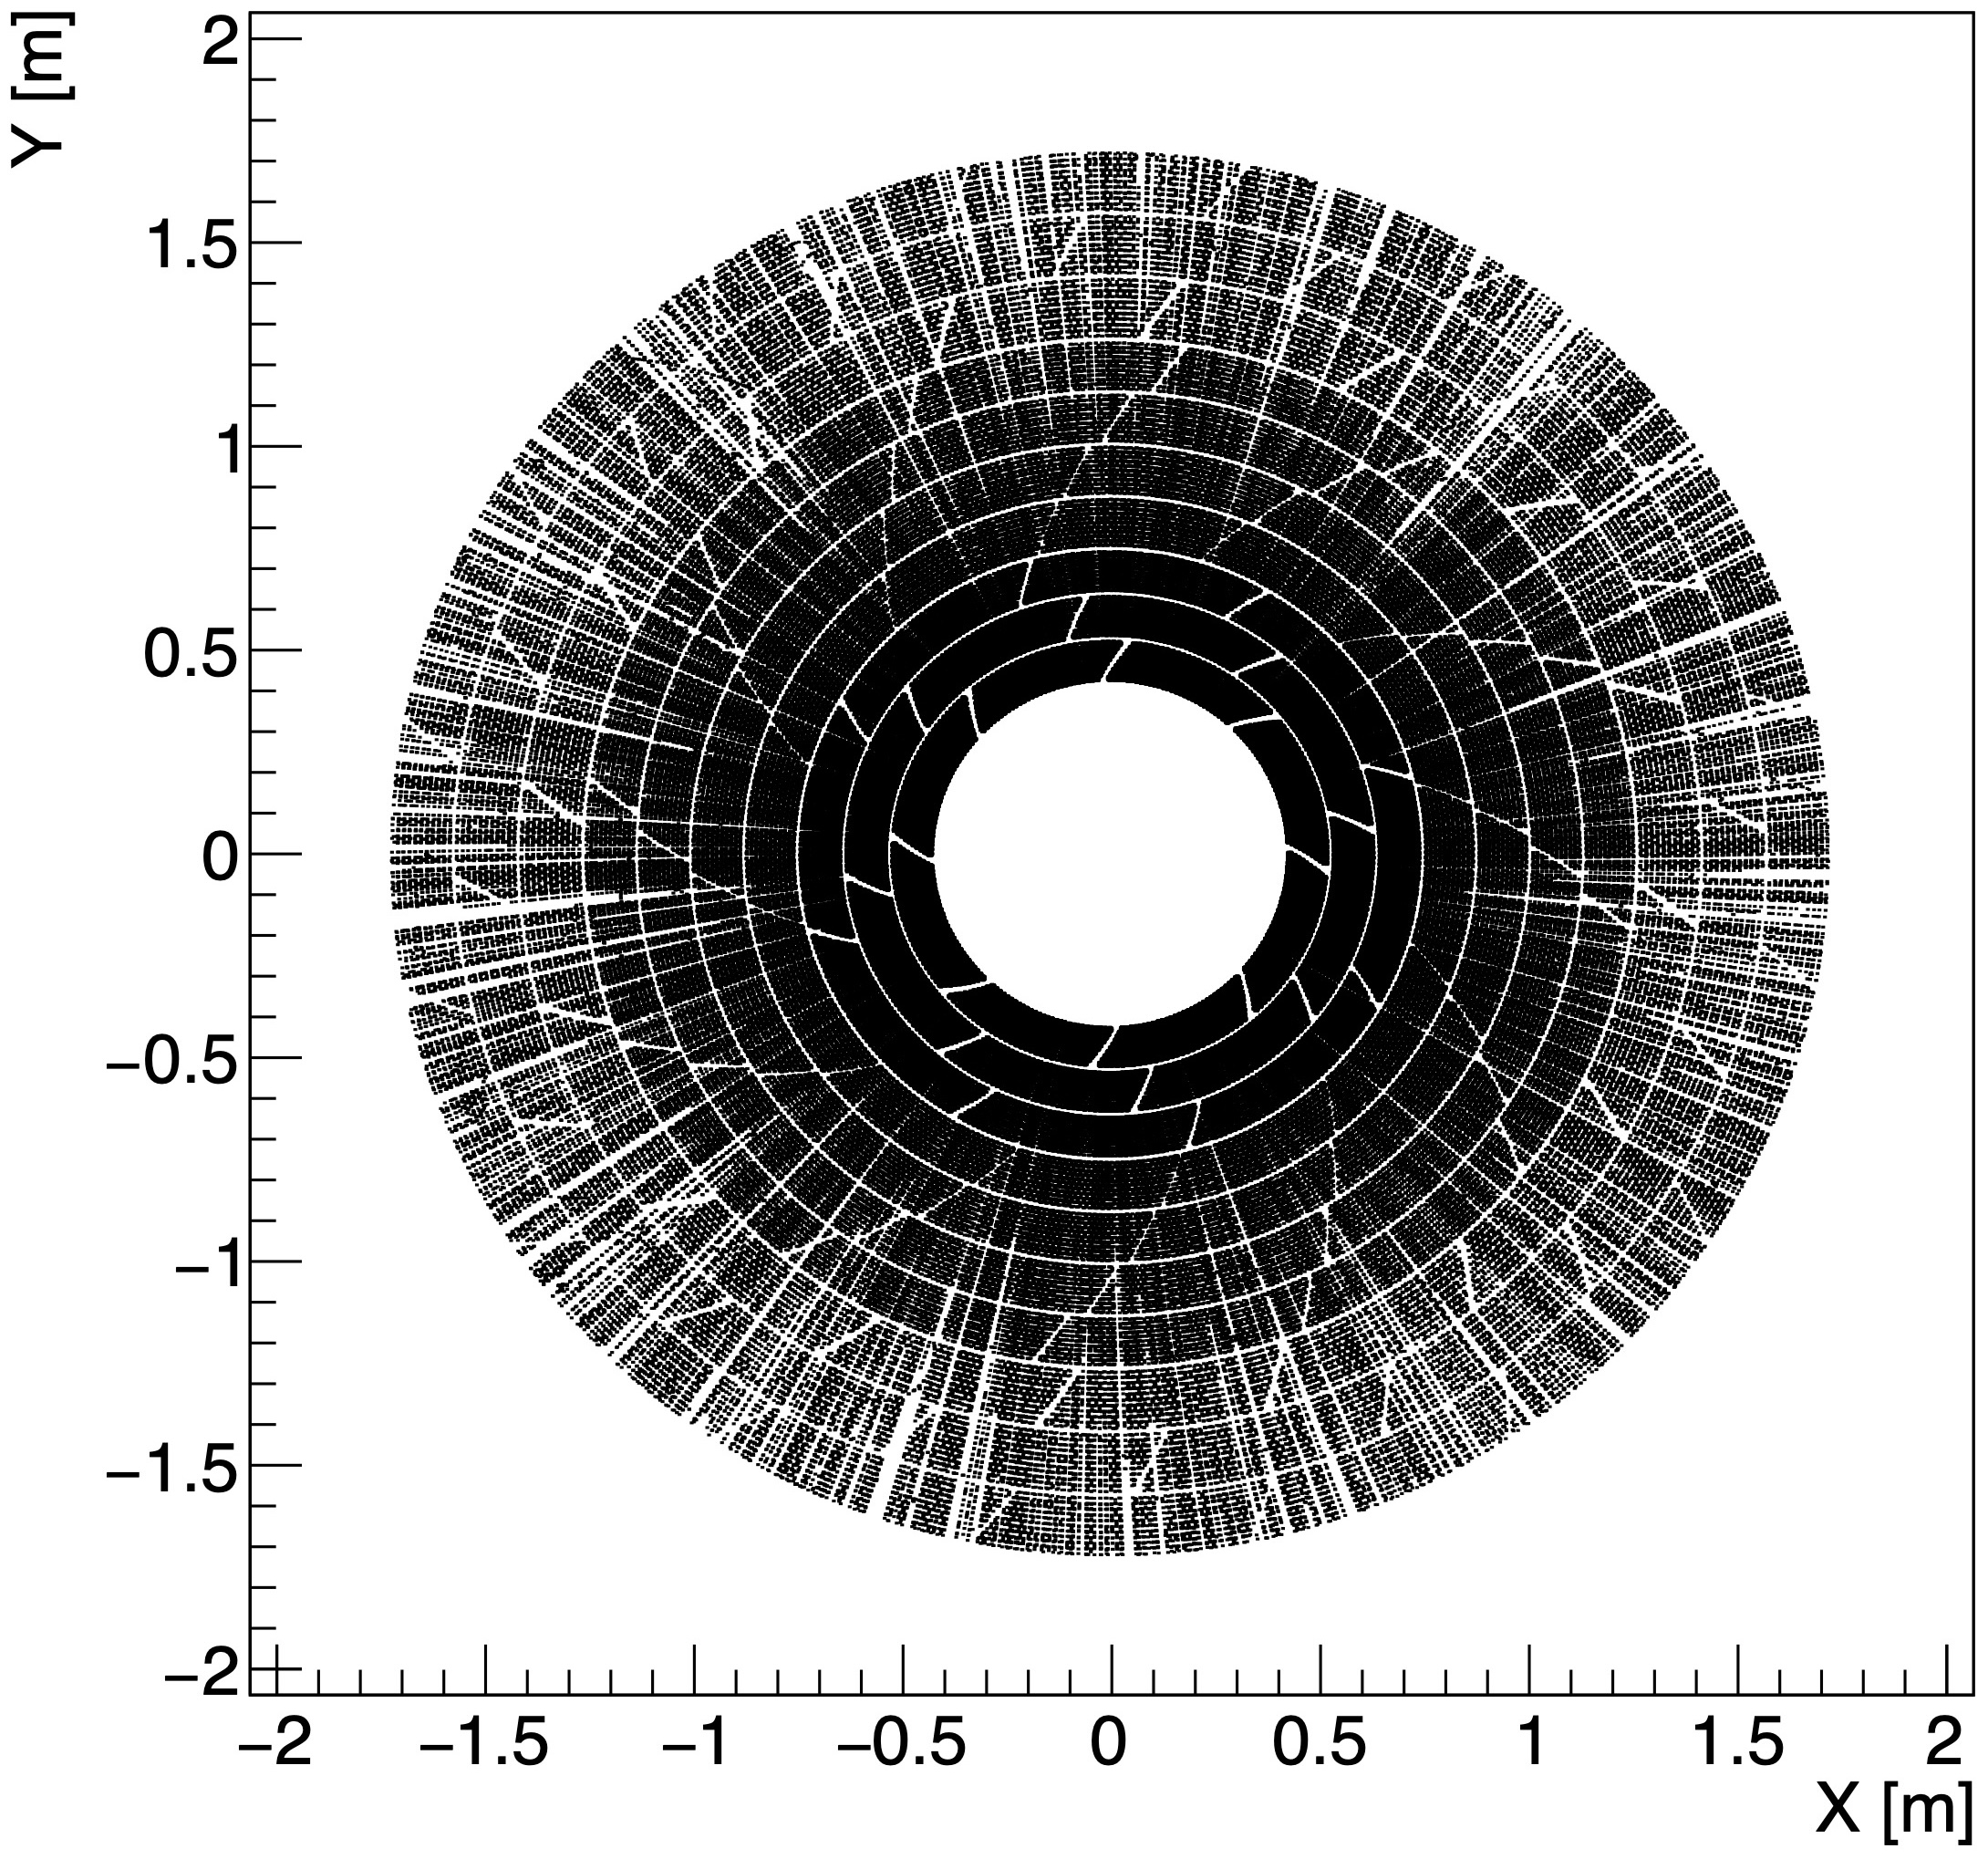
\includegraphics[width=0.4\linewidth]{Physics/DetectorConcepts/Figs/StrawTracker-layout-Geant.jpg}
\caption{(Left) An example layout of the straw tracker with ten superlayers, 
each superlayer containing ten sublayers.
(Right) Simulated hits from 5000 muons, revealing the layout of the straw tracker in the \textsc{Geant4} simulation.}
\label{fig:straw_tracker}
\end{figure}

Significant R\&D is required to realise such a detector design. 
Close collaboration with straw manufacturers is essential to produce ${\cal{O}}(12)$\,$\mu$m-thick-walled aluminium-coated straws with high yields. 
Optimising the detector layout and developing a robust mechanical design for the end-plates and support structure of these 5\,m-long straws are critical tasks. 
Further investigations into gas mixtures, \textsc{Garfield} simulations, and front-end electronics are important for d$E$/d$x$ and d$N$/d$x$ measurements. 
Fast algorithms need to be developed and implemented in the front-end ASIC or FPGA in order to effectively identify individual clusters.
In the coming years, prototype chambers will be built and tested with cosmic-ray muons and with beams, in view of validating the simulated performance.

\subsubsection{Time projection chamber}

Time projection chambers (TPCs) provide continuous 3D tracking over a large volume with minimal material interference, 
while also enabling particle identification via energy deposition in the gas. 
The gas choice is critical to maximise ionisation signal yield and minimise transverse diffusion, 
which strongly depends on the magnetic field strength and on the drift velocity. 
Minimising transverse diffusion calls for a `hot gas', commonly achieved so far with a small admixture of CF$_4$. 
Given that CF$_4$ has a strong greenhouse effect, a replacement gas will have to be identified. 
For particle identification via cluster counting, d$N$/d$x$, small, sub-millimetre pad sizes are needed, in which case digital readout is sufficient.

Mechanical alignment must be precise, within a few tens of microns, to avoid systematic errors. 
Electric and magnetic fields must be parallel, to prevent $E \times B$ distortions, calling for a highly uniform magnetic field. 
Minimising space-charge build-up is essential, as transverse electric field components distort electron drift paths. 
Hence, beam backgrounds 
(such as low-energy X-rays and muons from beam-halo interactions, both generating low-\pt particles that curl and deposit significant ionisation) 
must be controlled, or corrective strategies must be implemented. 
First estimates of the effect of beamstrahlung backgrounds were recently presented~\cite{DJeansECFA-Paris}, 
with the conclusion that distortions expected with the FCC-ee Tera-\PZ luminosities are at the same level as those observed in ALICE.
%
Ion feedback, where ions from the amplification process drift towards the cathode (over $\sim$\,0.5\,s), must be carefully managed. 
Operating at low gain with effective passive backflow mitigation, 
such as double misaligned meshes or graphene filters, would be necessary. 
If space charge effects are unavoidable, correction techniques (built on the experience of ALICE) should be employed.
%
The operability of a TPC at FCC-ee luminosities is still under discussion in the community and is being actively investigated. 

\subsection{Particle identification}

The identification of charged hadrons (\PGp, \PK, \Pp) 
significantly enhances the physics potential of experiments at FCC-ee, as discussed in Section~\ref{sec:PhysPerf_PID}.  
In particular, it improves the flavour-tagging performance in the selection of 
Higgs boson decays to $\PQc\PAQc$ or $\PQs\PAQs$, 
and is crucial for the extensive flavour physics programme with the \PZ-pole data. 
From simulation studies, the momentum region to be covered is up to a few tens of GeV.
For experiments with gaseous trackers, 
the specific energy loss (d$E$/d$x$) provides separation power up to moderate momenta, 
in conjunction with time-of-flight to cover the overlap region around 1\,GeV, where the d$E$/d$x$ separation is poor. 
As already mentioned for drift chambers or straw trackers, the performance can be enhanced with cluster counting, d$N$/d$x$. 
For experiments with silicon-based tracking, however, neither d$E$/d$x$ nor d$N$/d$x$ would provide the required level of performance. 
There, ring-imaging Cherenkov (RICH) detectors could deliver particle identification over a very wide momentum range. 
The following two sections describe the use of precision timing and RICH detectors 
to enable the required particle identification performance. 

\subsubsection{Precision timing detector}

The identification of charged hadrons based on their specific energy loss 
must be complemented by other measurements to fill the gap around 1\,GeV, 
where the Bethe--Bloch energy-loss curves for the different particle types cross over. 
Time-of-flight measurements, for example in a layer of silicon sensors at 2\,m from the interaction point, 
with a non-challenging resolution of $\sim$\,100\,ps, are adequate for this purpose. 
With a resolution of 30\,ps, 
time-of-flight measurements alone would allow kaons to be separated from pions up to ${\cal{O}}(3)$\,GeV in momentum, 
while an excellent resolution of 10\,ps would be needed to extend this momentum range up to 5\,GeV.
Such TOF information could also be obtained in a silicon-tungsten ECAL, 
where measurements, each of a resolution of, e.g., 100\,ps, could be made in several layers.  
Dedicated timing layers made of inorganic scintillator offer another solution. 
An example is the segmented crystal ECAL design of MAXICC (described in Section~\ref{sec:ECALs}), 
which includes two such thin layers, potentially providing a 20\,ps timing resolution. 

Because of the finite length of the colliding bunches, the `event time', $t_0$, has a natural spread of about 36\,ps at the \PZ pole. 
To exploit timing resolutions better than that value, $t_0$ needs to be determined on a event-by-event basis. 
In events with a high charged-particle multiplicity, 
it is possible to reconstruct $t_0$ from the timing measurement of the other tracks. 
For lower multiplicity events, e.g., $\PZ \to \PGt\PGt$, this method is less effective. 
As an alternative, an additional timing measurement close to the interaction point could be established, 
possibly in the form of an LGAD silicon sensor layer at low radius. 
This solution would allow a direct track-by-track time-of-flight measurement independent of $t_0$. 
Studies are needed in order to quantify the implications of such a layer in terms of 
additional material for readout electronics and cooling.

\subsubsection{Compact RICH detector}
\label{sec:ARC}

Studies are underway to develop a compact RICH detector for inclusion in CLD, 
with the goal of fitting it in a 20\,cm radial envelope and contributing less than 10\% of a radiation length to the material budget, 
hence limiting its impact on the other subsystems of the experiment, such as tracking and calorimetry. 
It is enabled by the new generation of photodetectors, in particular silicon photomultipliers (SiPM), 
that hold the promise of providing high detection efficiency and spatial granularity in a low thickness. 
A focusing geometry has been developed, 
where the surface of the detector is tiled with a large number of similar RICH detector elements, 
in a cellular approach, a concept named ARC, for `Array of RICH Cells'~\cite{Forty_ARC, Tat_ARC, forty_2024_6g0gs-7kw30}.

\begin{figure}[t]
\centering
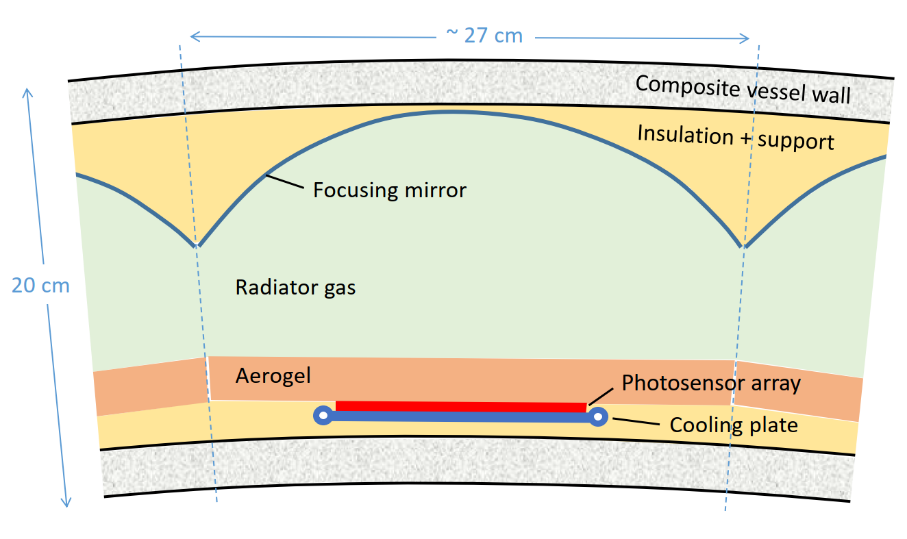
\includegraphics[width=0.5\linewidth]{Physics/DetectorConcepts/Figs/ARC-schematic.png} \\ 
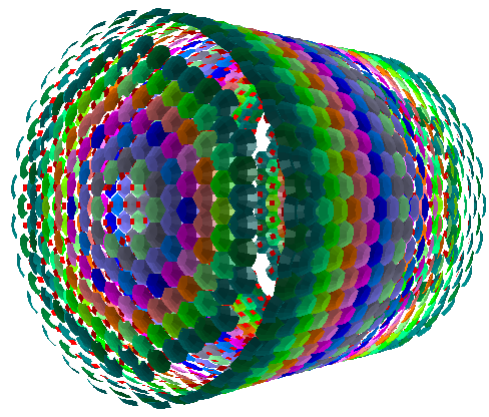
\includegraphics[width=0.38\linewidth]{Physics/DetectorConcepts/Figs/ARC-layout.png} \hglue5mm
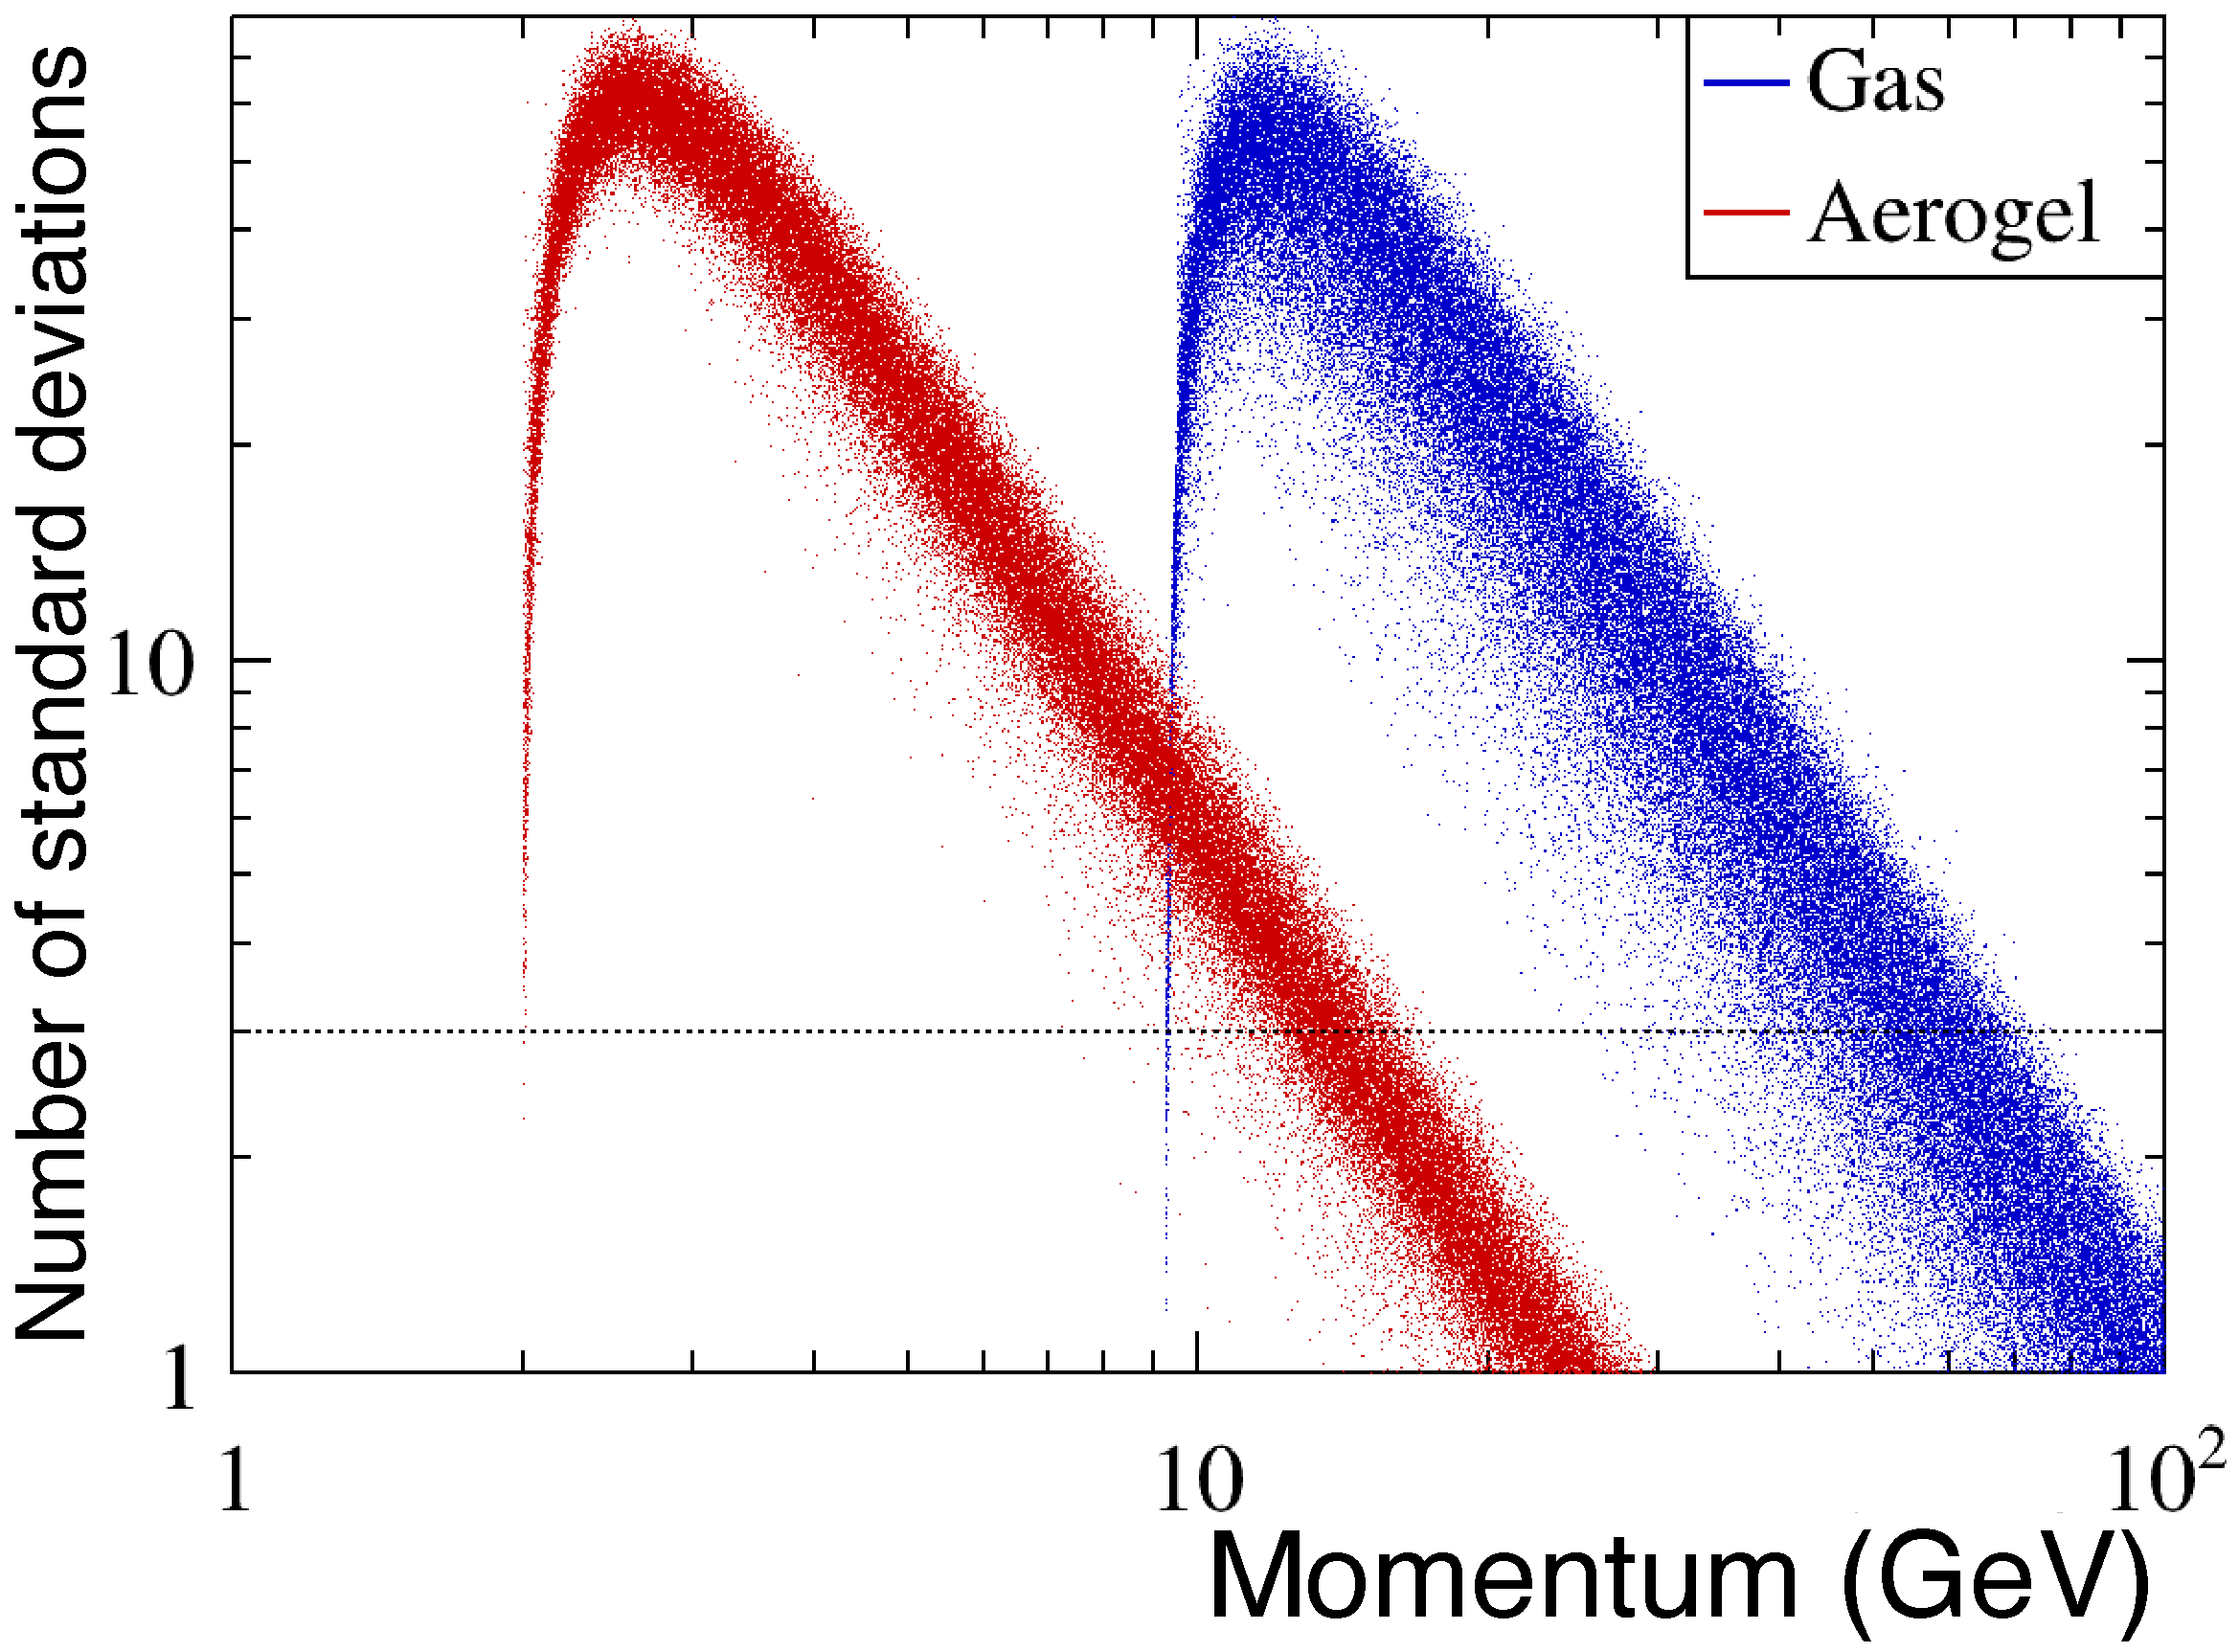
\includegraphics[width=0.45\linewidth]{Physics/DetectorConcepts/Figs/ARC-performance-CL.pdf}
\caption{Top: Schematic cross section through the ARC barrel detector, 
showing the various components of a single cell.
Bottom left: ARC barrel and end-cap as described in the detector geometry of the simulation,
with colours used to distinguish the cells. 
Bottom right: Momentum dependence of ARC's \PK/\PGp separation (in standard deviations), 
with two radiator options.}
\label{fig:ARC}
\end{figure}

The components of an ARC cell are shown in the top panel of Fig.~\ref{fig:ARC}. 
The lightweight vessel is made of carbon-fibre composite, 
with a wall thickness that depends on whether the contained gaseous radiator needs to be pressurised. 
The RICH uses dual radiators, silica aerogel and gas, 
with Cherenkov photons from both radiators focused via a spherical mirror onto a common SiPM detector plane. 
The baseline choice for gaseous radiator is C$_{4}$F$_{10}$ at atmospheric pressure, 
given its attractive optical properties, as used for example in the RICH1 detector of LHCb, 
aiming for a leak-free closed circulation system. 
With the high photon-detection efficiency achievable with SiPMs, 
this option can provide a sufficient number of detected photons, about 16 for a high-momentum particle, 
despite the limited radiator length of only around 15\,cm. 
On the timescale of FCC, however, such fluorocarbons may be banned, 
so that R\&D is required to find alternative gases, such as xenon with mild pressurisation, 
to ensure a sufficient yield of detected photons. 
The aerogel radiator extends the particle identification performance to low momenta, 
while also serving as an efficient thermal insulator, 
separating the gas radiator from the SiPM detector plane, 
which is likely to need cooling to limit the dark-count rate 
(although the option of suppressing noise with timing cuts will also be investigated). 
This insulator would allow the SiPMs to be operated at around $-40$\,$^\circ$C, 
e.g., with mixed-phase CO$_2$ circulation, 
while maintaining the radiator gas at room temperature to prevent condensation.

The performance of such a RICH concept has been evaluated with full simulation studies~\cite{Delgado_ARC}. 
The geometry of each cell, in terms of mirror and photodetector position and angle, 
depends on the position of the cell in the detector.  
Given symmetry considerations, there are about 40 unique cell geometries across the detector, 
which have been optimised in an automated procedure. 
The resulting detector description has been implemented in the \textsc{Key4Hep} software framework (Chapter~\ref{sec:software}), 
with \textsc{DD4hep} for the geometry and \textsc{Geant4} for the simulation, 
as illustrated in the bottom-left panel of Fig.~\ref{fig:ARC}. 
Taking the integration into CLD as an example, 
10\% of the original tracker volume has been reassigned to ARC, 
the tracker dimensions being adapted to fit in the remaining space. 
Studies are underway to develop pattern recognition and particle identification algorithms, 
as well as to check the impact on the experiment, e.g., on the performance of the tracking and particle-flow calorimetry. 
Meanwhile, the performance has been studied using standalone ray-tracing software, 
as shown in the bottom-right panel of Fig.~\ref{fig:ARC}.
The overall resolution per detected photon is around 2\,mrad, 
balanced between contributions from the chromatic dispersion, focusing errors, and pixel size, 
where mm-scale pixelisation of the SiPMs has been assumed. 
Excellent \PK/\PGp separation is achieved for momenta above 2\,GeV. 
For lower momenta, a TOF system would provide complementary information. 
The development of ARC is established as a task within the newly formed DRD4 collaboration~\cite{Easo_DRD4}, 
with the milestone of a full conceptual design within a year 
and a prototype of a single ARC cell to be delivered within three years. 
Such a prototype will provide an excellent test-bed for the study of the key developments required for this detector,
as well as the possibility of including RICH detectors as integral parts of the FCC-ee tracking detectors.

\subsection{Electromagnetic calorimeters}
\label{sec:ECALs}

\subsubsection{Silicon pads, MAPS, scintillator strips}

Electromagnetic calorimeter technologies with embedded front-end electronics 
and high 3-dimensional segmentation have been studied extensively~\cite{Sefkow:2015hna}. 
They include silicon pads, MAPS sensors and scintillator strips, 
and capitalise on the possibility of power-pulsing and overall modest bandwidth requirements. 
Adapting them to a circular collider such as FCC-ee, with continuous readout and high rates, 
poses challenges for data concentration, powering, and cooling, 
requiring a full re-optimisation to maximally preserve their compactness. 
Silicon diodes are currently implemented in the CMS end-cap calorimeter upgrade, 
but the FCC-ee goals in terms of compactness (Moli\`ere radius), 
energy resolution, and granularity are considerably more ambitious. 

Related R\&D has begun, in the framework of the DRD6 Collaboration. 
As a first step, quantitative requirements are being studied in simulations. 
Tools have been developed to evaluate hit occupancy, bandwidth and, 
with model assumptions on the embedded electronics, 
power consumption as a function of position in the detector~\cite{Hassouna:2024frw}.

\subsubsection{Noble liquid}
 
The proposed ALLEGRO noble-liquid electromagnetic calorimeter is a sampling detector 
using liquid argon as active medium and lead/steel absorbers as passive material. 
The absorbers and electrodes are straight, and inclined (in the barrel) in the ($x,y$) plane 
by 50$^\circ$ with respect to the radial direction. 
The detector has both transverse and longitudinal segmentation.
Alternative design options include liquid krypton as active medium and tungsten for passive material, 
as well as trapezoidal absorbers to maintain the sampling fraction constant as a function of depth.

The calorimeter is located inside a cryostat, 
made of 33.8\,mm-thick aluminium in the current simulations 
while novel, lightweight materials are being considered (Section~\ref{sec:Cryostat}).
The 2\,mm-thick absorber plates are composed of a sandwich of lead (1.8\,mm) with steel sheets glued on either side.
Between adjacent absorbers are two equal-size liquid argon gaps, 
separated from each other by a 1.2\,mm-thick electrode, realised as a multilayer PCB.
The use of multilayer PCBs as readout electrodes allows for great flexibility in the choice of granularity as a function of depth.
In the present geometry, the liquid argon gaps have thicknesses, 
projected along the direction orthogonal to the electrode,
of $2 \times 1.25$\,mm at the inner radius and $2 \times 2.43$\,mm at the outer radius.
The electrodes are segmented longitudinally into 11 layers.
The first layer, about half as thick (1.5\,cm) as the others (3 to 5\,cm), is used as a presampler. 
To achieve a $\phi$-uniform response of that first layer, 
the absorber does not contain lead, to form a `LAr-only' homogeneous presampler.
The sampling fraction is about 38\% in the presampler layer 
and increases from 13.5\% to 17.3\% throughout the other 10 layers.
A depth of 22\,$X_0$ is achieved in a thickness of 40\,cm for the Pb--LAr solution 
and about two thirds of that for denser solutions based on W and LKr.


The segmentation in $\phi$ is naturally provided by the absorbers.
The baseline is to read out two gaps together, forming a single cell spanning $\Delta\phi = 2\pi/768 = 8$\,mrad. 
The segmentation along the electrode and in $\theta$ is formed by cells on the readout electrode.  
It amounts to $\Delta\theta = 0.56^\circ$, except in one of the first layers, 
where a four-times finer granularity ($\Delta\theta = 0.14^\circ$) is implemented, 
to discriminate between single showers from prompt photon and collimated pairs of showers from neutral pion decays. 
The total number of readout channels for the barrel part of the calorimeter is around 2~million.
The expected sampling term of the resolution ranges from $\sim$\,7.5\%/$\sqrt{E}$ for a solution based on LAr, 
down to below 5\%/$\sqrt{E}$, for a denser solution based on LKr.

An adapted geometry is needed for the detector end-caps. 
The inclined absorber and electrode planes of the barrel calorimeter are replaced by `blades' arranged in a turbine-like structure. 
In order to avoid having too large variations of gap sizes and sampling fractions between the inner and outer radii, 
the detector is assembled as three nested wheels, with similar gap sizes at the inner radius of each wheel.

The geometries of both the barrel and the end-cap sections are implemented 
in the \textsc{Geant4} full simulation of the \textsc{Key4Hep} software framework. 
Algorithms for digitisation and clustering (fixed-size sliding-window and topological clusters) are also implemented. 
Example displays of reconstructed clusters from single-photon and single-\PGpz events are shown in Fig.~\ref{fig:ALLEGRO_ECAL_eventdisplays}.

\begin{figure}[h]
\centering
\includegraphics[width=0.45\textwidth]{Physics/DetectorConcepts/Figs/Allegro-ECAL-display-photon.jpg}
\includegraphics[width=0.45\textwidth]{Physics/DetectorConcepts/Figs/Allegro-ECAL-display-pi0.jpg}
\caption{Event displays in the ($r,z$) view for clusters reconstructed in the ECAL barrel of ALLEGRO, 
for a photon (left) and a $\PGpz \to \PGg\PGg$ (right), 
both coming from the main IP at normal incidence with an energy of 10\,GeV. 
The particles impinge on the detector from the bottom. 
Clustered cells are shown in brown, with lighter tones corresponding to higher cell energies.
The yellow dots are placed in the cell centres. 
Noise is not simulated.
In this simulation, the strip layer is the first one.}
\label{fig:ALLEGRO_ECAL_eventdisplays}
\end{figure}
\begin{figure}[h]
\centering
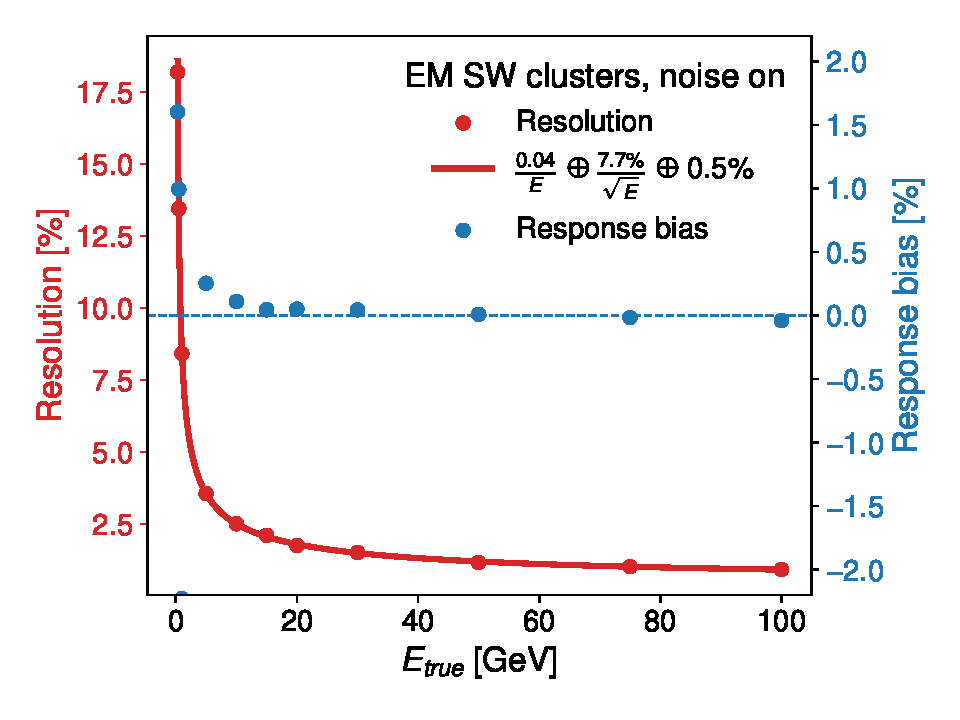
\includegraphics[width=0.4\textwidth]{Physics/DetectorConcepts/Figs/Allegro-ECAL-resolution_and_response_vs_energy_cal_EMBCaloClustersWithNoise.pdf}
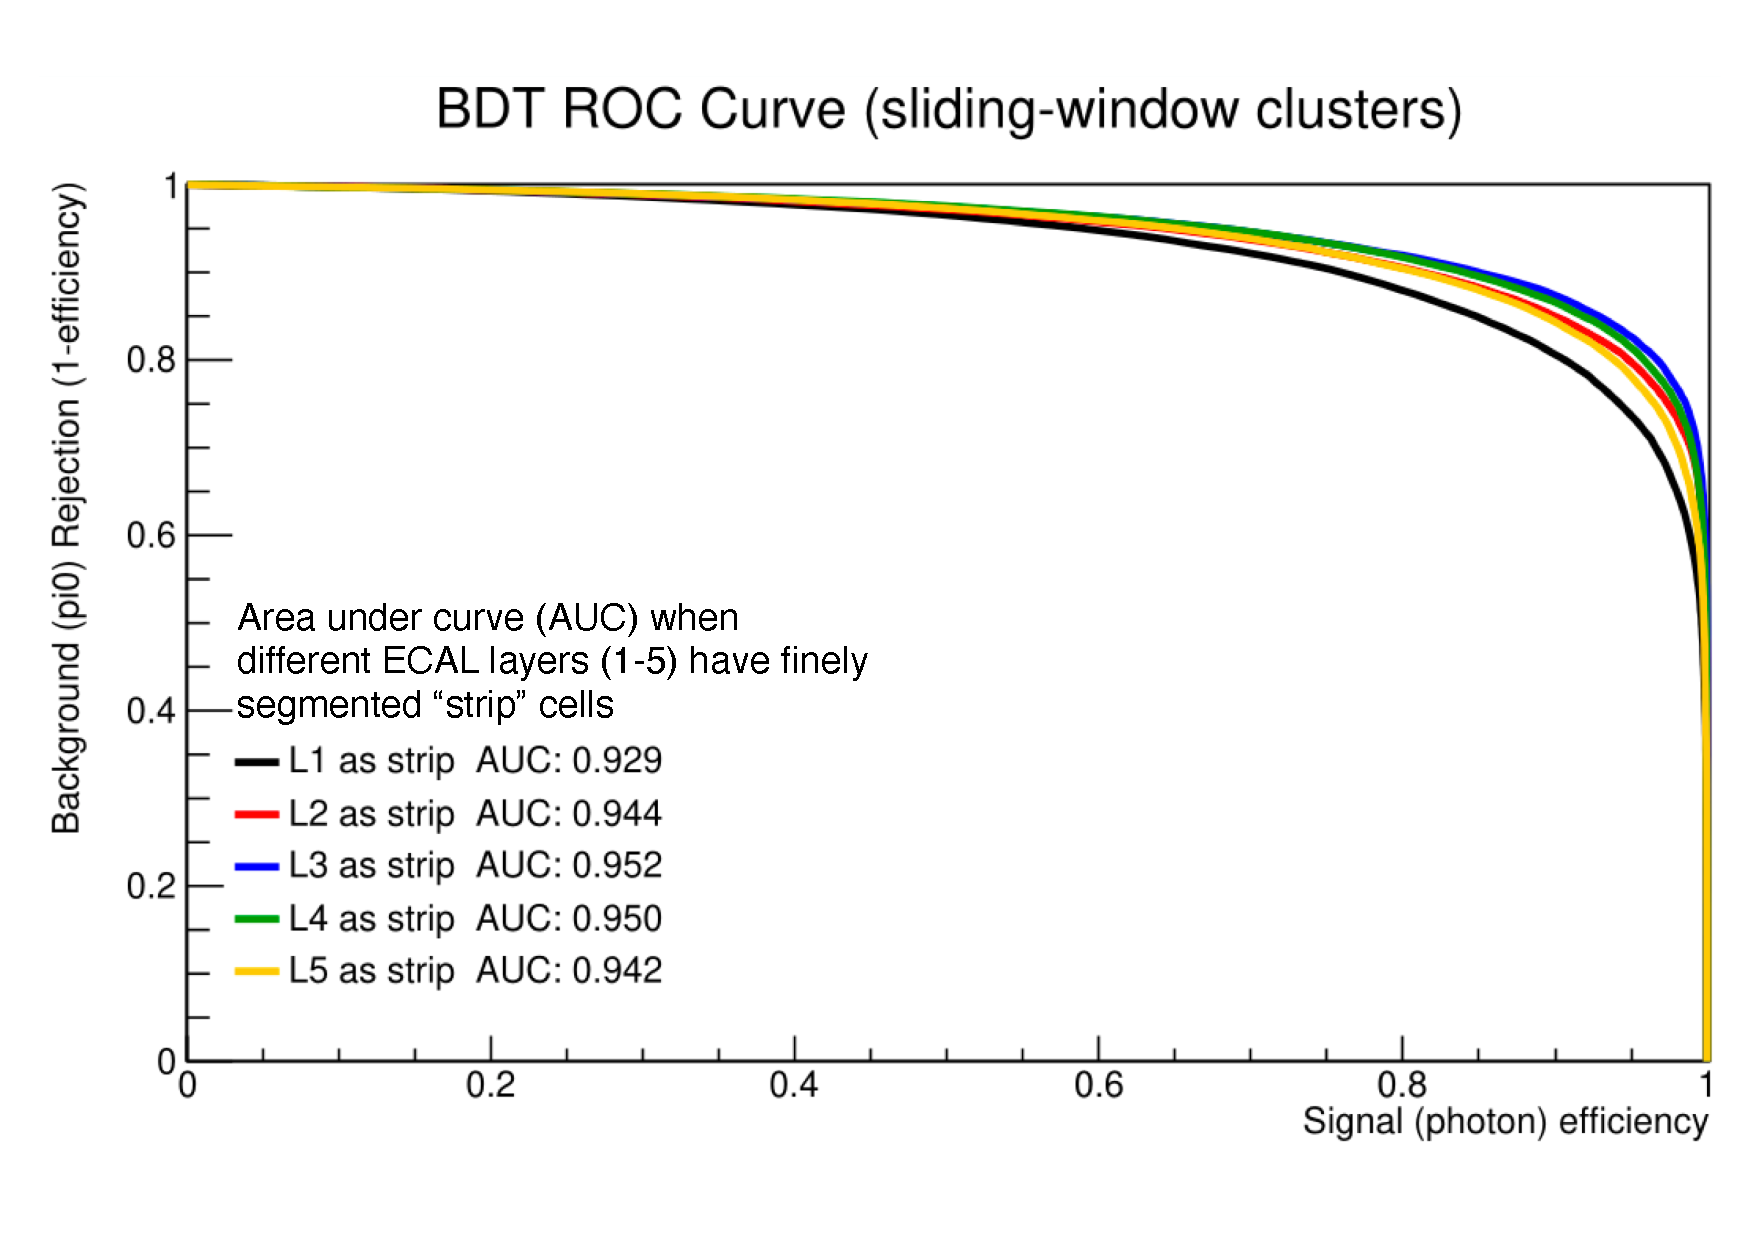
\includegraphics[width=0.5\textwidth]{Physics/DetectorConcepts/Figs/Allegro-ECAL-photon-vs-pi0.pdf}
\caption{Left: Simulated energy response and resolution of the LAr ECAL barrel calorimeter, including noise, 
for reconstructed (sliding window) photon clusters as a function of the true photon energy.
Right: ROC curves of a BDT trained to discriminate between photons and neutral pions with momenta between~1 and~100\,GeV, using input features calculated from the clustered cell energies. }
\label{fig:ALLEGRO_ECAL_performance}
\end{figure}

Examples of performance studies are illustrated in Fig.~\ref{fig:ALLEGRO_ECAL_performance}, 
where the energy resolution and response expected with the (LAr plus tungsten) baseline model are shown, 
together with the ROC curves for a simple BDT-based photon/\PGpz discrimination algorithm 
exploiting the shower shapes computed from the cell energies. 
The latter, which shows the area-under-curve (AUC) of the efficiency vs.\ rejection curve of the BDT algorithm 
for various alternative configurations corresponding to different positions of the strip layer, 
demonstrates how the simulation can help design choices.

Sustained R\&D on noble liquid calorimeters is carried out in the framework of the WP2 of DRD6. 
Ongoing activities focus on the optimisation of the detector material, geometry and segmentation, 
overall detector mechanical structure and integration, readout electronics, 
as well as on prototyping and testing the various detector elements. 
On a longer timescale, the plan is to build a prototype and test it with beam, around 2027--2028.

\subsubsection{Segmented crystals with dual-readout}
\label{sec:Segmented-crystals}

The Maximum Information Crystal Calorimeter (MAXICC) 
is a homogeneous electromagnetic calorimeter concept optimised for FCC-ee,
made of longitudinally segmented crystals with embedded dual-readout and precise timing capabilities. 
An overview of its design can be found in Ref.~\cite{Lucchini:2020bac}.
This calorimeter offers an electromagnetic energy resolution of $3\%/\sqrt{E}$, 
crucial for studies of heavy-flavour physics with low-energy final-state photons~\cite{RoyAleksan} 
and to improve the resolution of the mass recoiling against $\PZ \to \epem$ in $\PZ\PH$ events with a recovery of bremsstrahlung photons. 
Furthermore, it enables an efficient clustering of photon pairs from \PGpz decays, 
which can effectively reduce the splitting of the two photons across different jets in multi-jet events~\cite{Lucchini:2020bac}.

The MAXICC calorimeter design is optimised for integration with a dual-readout hadron calorimeter section 
to provide an energy resolution for charged and neutral hadrons of about $27\%/\sqrt{E} \oplus 2\%$,
by correcting each shower individually using its estimated electromagnetic fraction, 
simultaneously measured with different techniques, 
thereby reducing the impact of shower fluctuations on the resolution. 
The inclusion of longitudinal segmentation and the enhancement of transverse granularity with $\sim$\,1\,cm$^2$ cells 
(compared to the previous generation of crystal calorimeters) 
provide a powerful handle for particle identification 
and association of charged-particle tracks with calorimeter clusters in particle-flow jet reconstruction, 
with the potential to achieve an energy resolution of 4.5\% for 45\,GeV jets~\cite{Lucchini_2022}, 
as shown in Fig.~\ref{fig:drpfa_jetres}.
A complete simulation of the detector integrated with other IDEA sub-detectors,
within the \textsc{Key4hep} framework, 
is in progress, to allow more detailed physics studies~\cite{WonyongProceeding}.

\begin{figure}[ht]
\centering
\begin{minipage}[t]{0.48\textwidth}
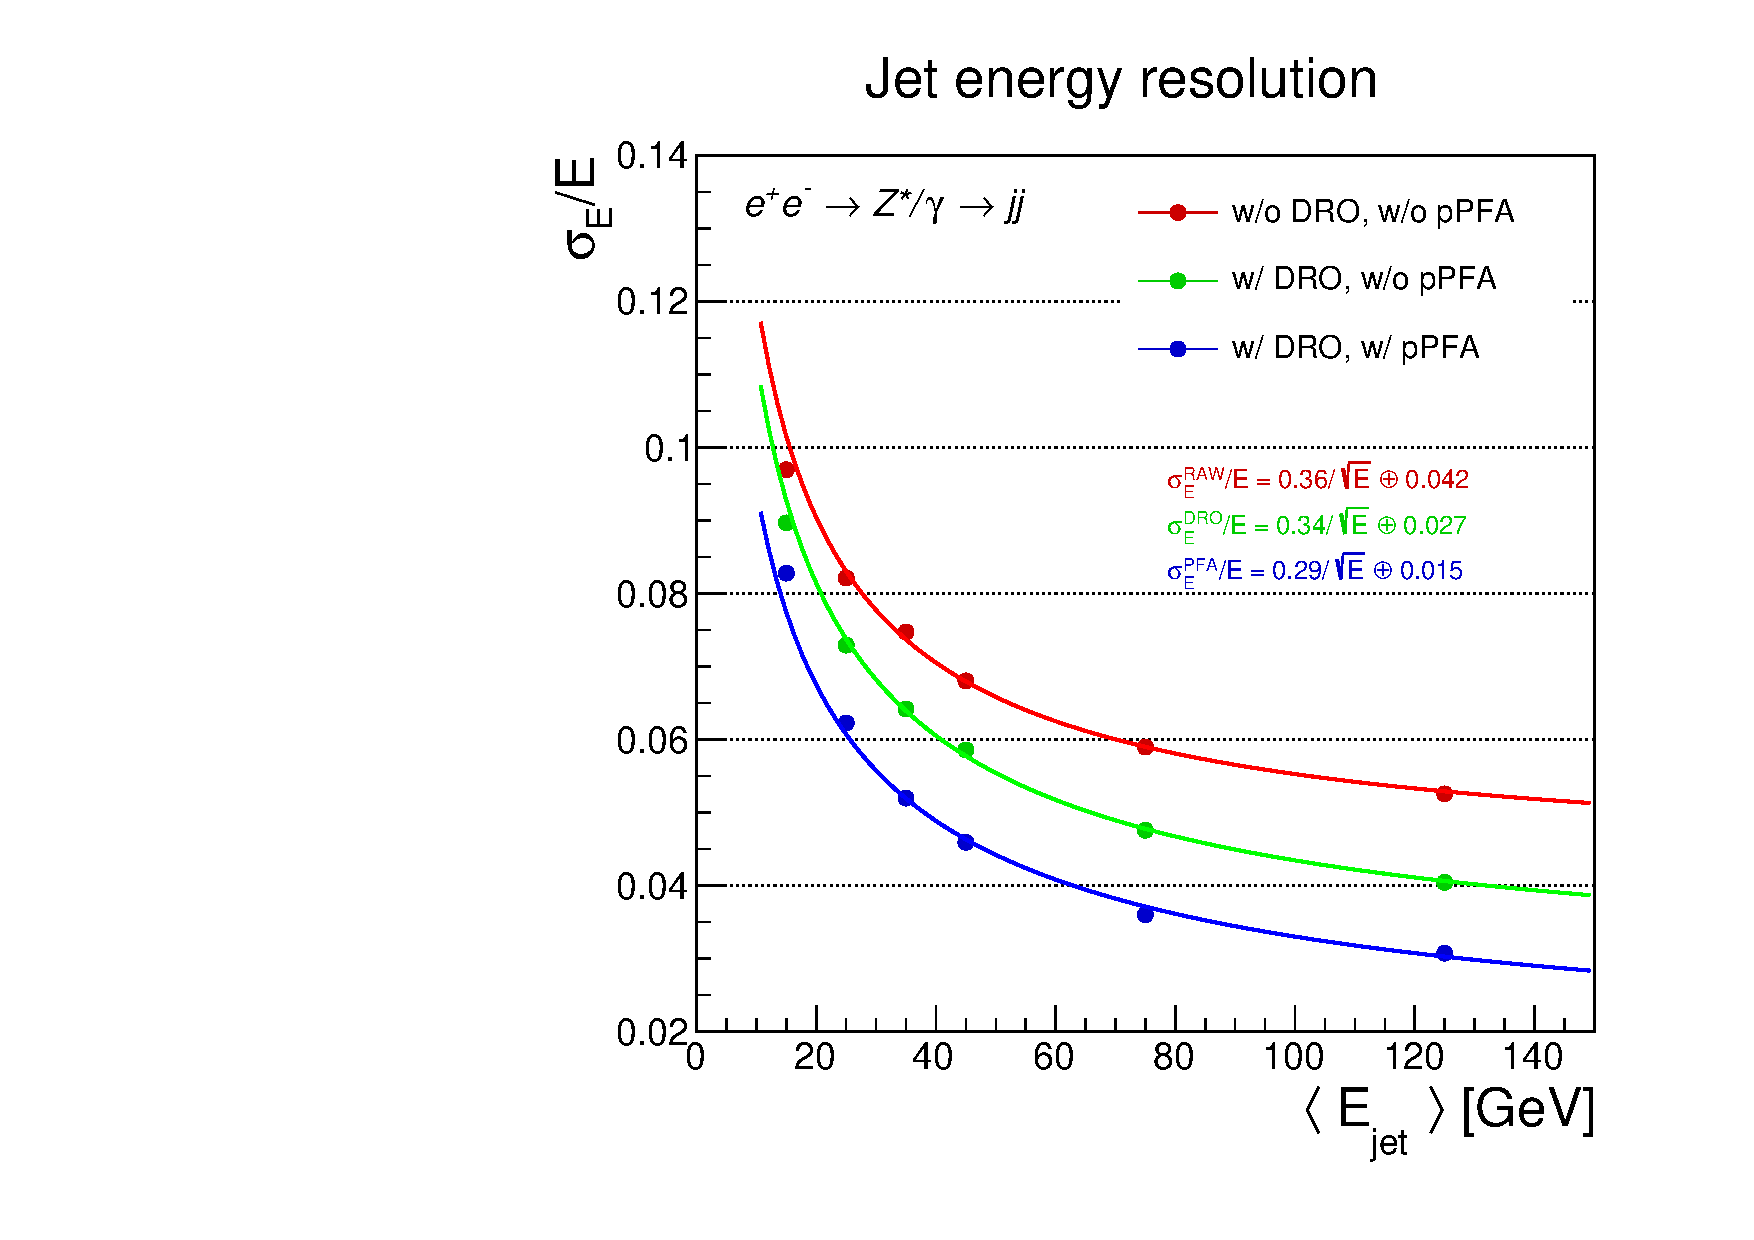
\includegraphics[width=\linewidth]{Physics/DetectorConcepts/Figs/cCompareRes_DRO_PFA_B2T__TRKSMEAR.pdf}
\caption{Jet energy resolution vs.\ 
jet energy, with or without a dual-readout particle flow algorithm.
}
\label{fig:drpfa_jetres}
\end{minipage}    
\hfill
\begin{minipage}[t]{0.48\textwidth}
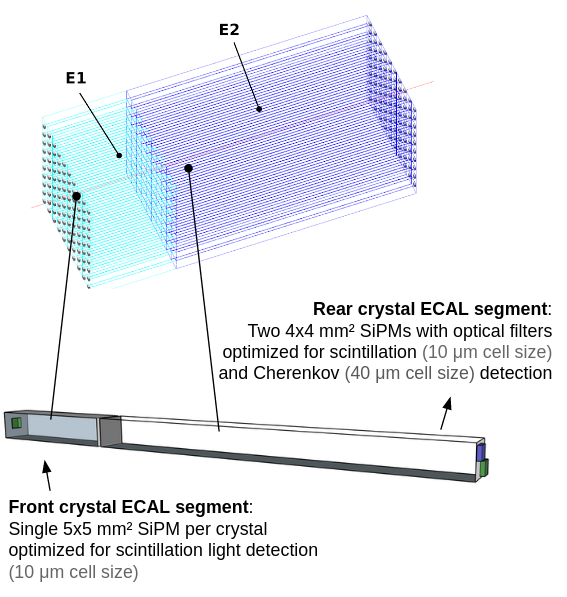
\includegraphics[width=\linewidth]{Physics/DetectorConcepts/Figs/module_cell_image.png}
\caption{Segmented crystal calorimeter prototype cell and module with SiPM dual-readout.}
\label{fig:maxicc}
\end{minipage}
\end{figure}

As shown in Fig.~\ref{fig:maxicc}, 
the baseline calorimeter design features two longitudinal layers of high-density crystals (such as PWO or BGO), 
with 6\,$X_0$ in the front layer and 16\,$X_0$ in the rear layer, 
for a total of 22\,$X_0$ to ensure full containment of electromagnetic showers. 
The light from the crystals is read out with silicon photomultipliers (SiPMs) of active area 
in the range between $4 \times 4$ and $6 \times 6$\,mm$^2$. 
One SiPM is glued on the front side of the front layer and two are glued on the rear face of the rear layer. 
One of the rear SiPMs embeds an optical filter that cuts out the scintillation light based on wavelength discrimination 
and detects a pure Cherenkov signal for dual-readout corrections.  
An alternate approach also uses pulse shape analysis to differentiate scintillation and Cherenkov components.  
The front-end boards, electronics, and cooling services are located in the front and rear parts of the calorimeter 
to minimise the impact of passive material on energy resolution.

The MAXICC calorimeter can provide a time resolution better than 30\,ps 
for electromagnetic showers with energy of 20\,GeV or higher,
as obtained from beam tests with similar calorimeter prototypes~\cite{FERRI2020162159}.
In addition, two thin and highly segmented layers of LYSO:Ce crystals, for a total of 1\,$X_{0}$, 
could be added in front of the PWO crystals for time tagging of minimum ionising particles, 
using a technology similar to that used by the CMS MTD~\cite{CMS_MTD_TDR},
with a time resolution of 20\,ps.

The required technological R\&D, prototyping, and simulation are progressing steadily, 
through a coordinated effort of many international collaborators within the DRD6 WP3 (task~3.1.2). 
Single calorimetric cells have been tested with beam in 2024 and full containment calorimeter prototypes 
(one using PWO and the other using BGO)
are being built for beam tests in 2025. 
Each prototype will instrument $\sim$\,100--200 channels for readout,
covering a transverse size of at least five times the Moli\`ere radius and a depth of $22\,X_0$.  

\subsubsection{The GRAiNITA ECAL}

The GRAiNITA concept features a novel electromagnetic calorimetry design,
with a detection volume filled with millimetric grains of high-$Z$ and high-density inorganic scintillator crystals 
immersed in a bath of transparent high-density liquid. 
The multiple refractions of the light on the grains ensure the stochastic confinement of the light, 
as in the LiquidO detection technique~\cite{LiquidO:2019mxd}. 
The scintillation light can be collected towards the photodetectors by means of WLS fibres, 
regularly distributed in the detection volume as for a conventional Shashlik detector, 
allowing a potentially-large transverse granularity. 
This extremely-fine sampling of the electromagnetic shower promises an excellent energy resolution,
comparable to what is known from crystal calorimeters.

The main high-$Z$ and high-density inorganic scintillator crystal considered for GRAiNITA is ZnWO$_4$~\cite{bib:IEEE2022}, 
providing a light yield of $\sim$\,10\,000 photons per MeV. 
A considerable advantage is that ZnWO$_4$ can be successfully grown in the form of transparent granules of the desired size, 
with the method of spontaneous crystallisation from a flux melt~\cite{bib:IEEE2022}, significantly reducing the cost of the calorimeter. 
Such a high energy-resolution granular calorimeter would then meet the requirements,
from physics and otherwise, of an FCC-ee experiment. 
It would, moreover, be particularly useful to address a comprehensive flavour physics programme 
with rare decays involving photons or neutral pions in the final state. 
Given that the \PZ production rate at FCC-ee is of the order of 100\,kHz
and since these events should typically hit less than 1\% of the calorimeter cells, 
the 20\,$\mu$s signal decay time of the ZnWO$_4$ should not be a concern. 
Nevertheless, the possible use of other types of crystals will be investigated. 

Measurements with a small prototype ($2.8 \times 2.8 \times 5.5$\,cm$^3$) equipped with a green LED confirm that, as expected, 
the signal remains confined in the vicinity of its production point~\cite{Barsuk_2024}. 
From the analysis of cosmic-ray muons~\cite{Barsuk_2024} and of data from a muon beam test performed in summer 2024 at CERN with the same small prototype, 
it is clear that the collection of about 10\,000 photo-electrons per GeV is within reach with a GRAiNITA-like calorimeter. 
This result paves the way for a statistical fluctuation of $1\%/\sqrt{E}$ on the energy resolution from photo-electrons (Fig.~\ref{fig:NPHE}). 
The next steps, following this proof-of-principle, include the system aspects, including a mechanical configuration and an electronics read-out concept.

\begin{figure}[ht]
\centering
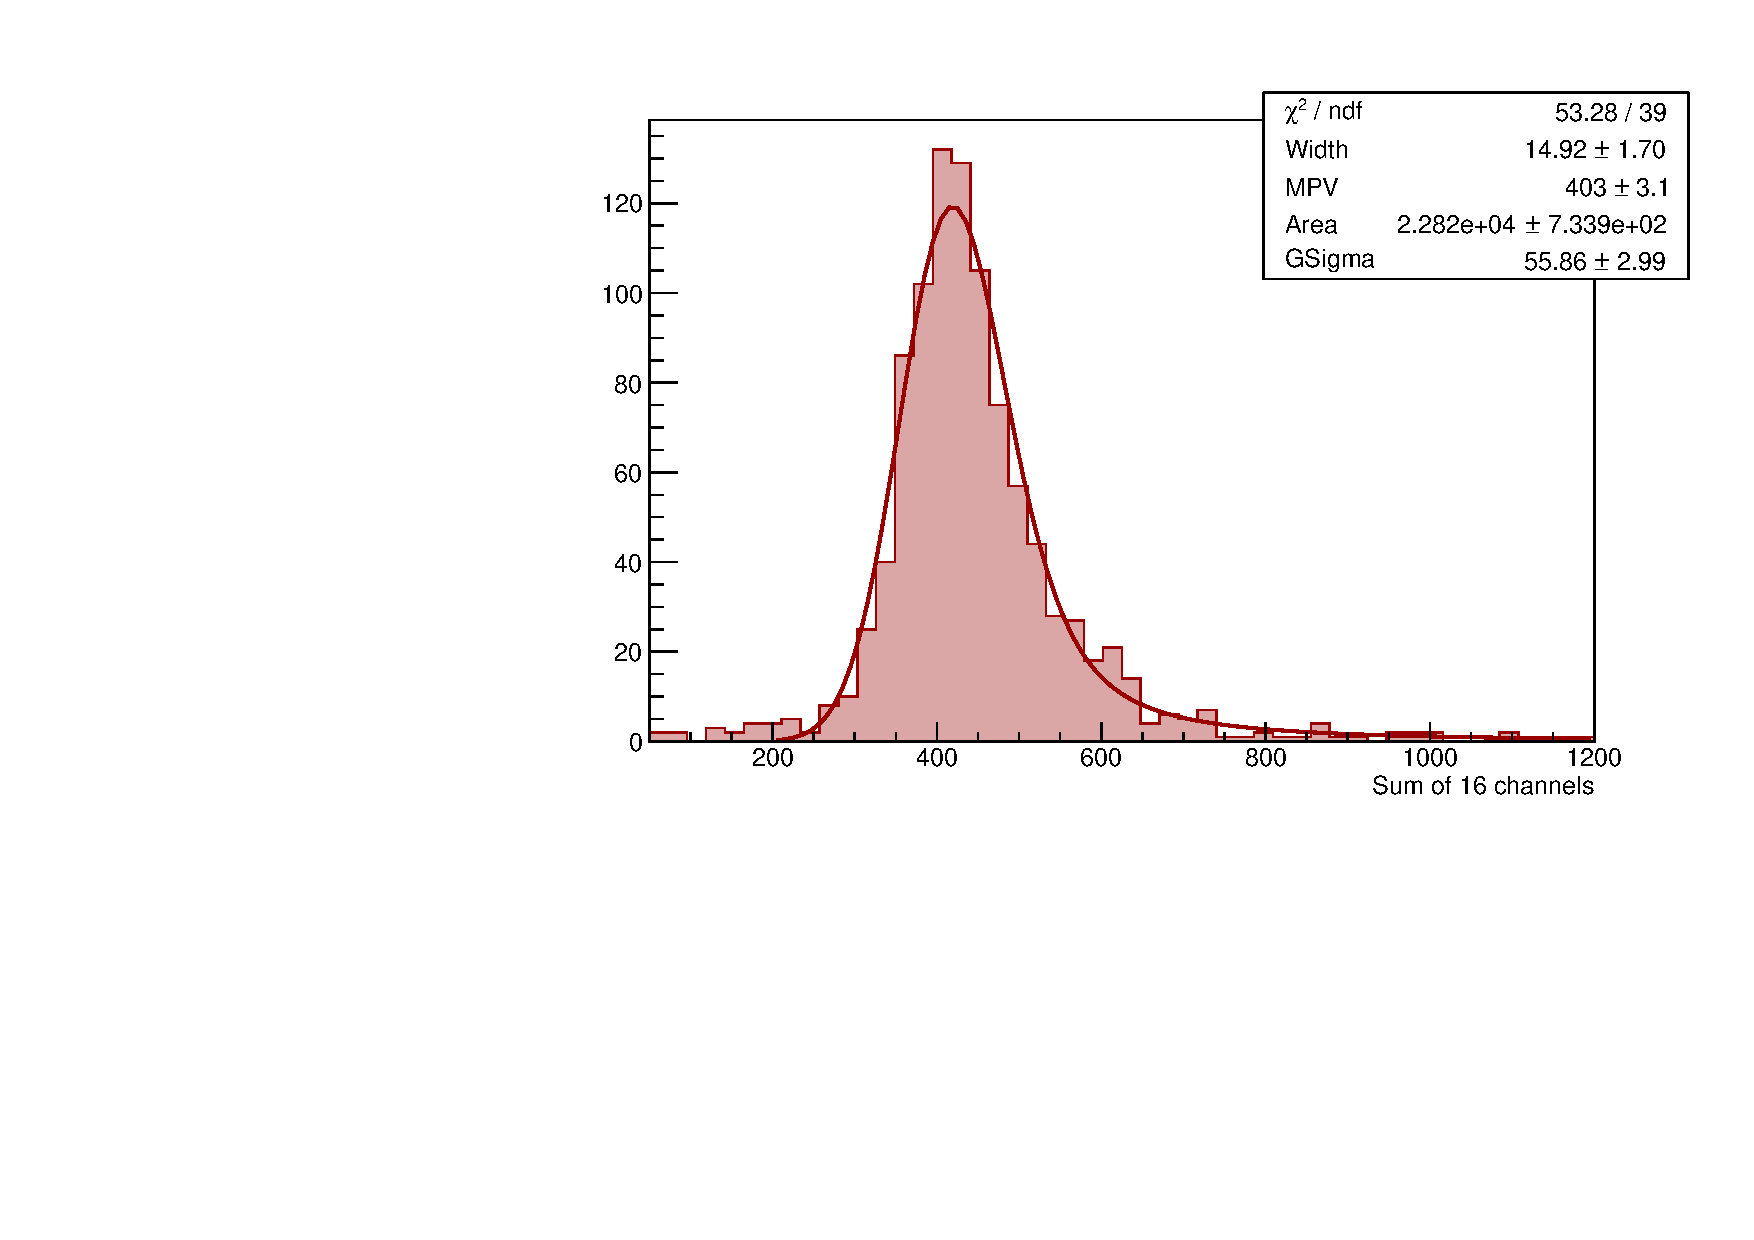
\includegraphics[width=.45\textwidth]{Physics/DetectorConcepts/Figs/Run_Cosmic_Pub_ZWO_EGL_FitSumCorr.pdf}
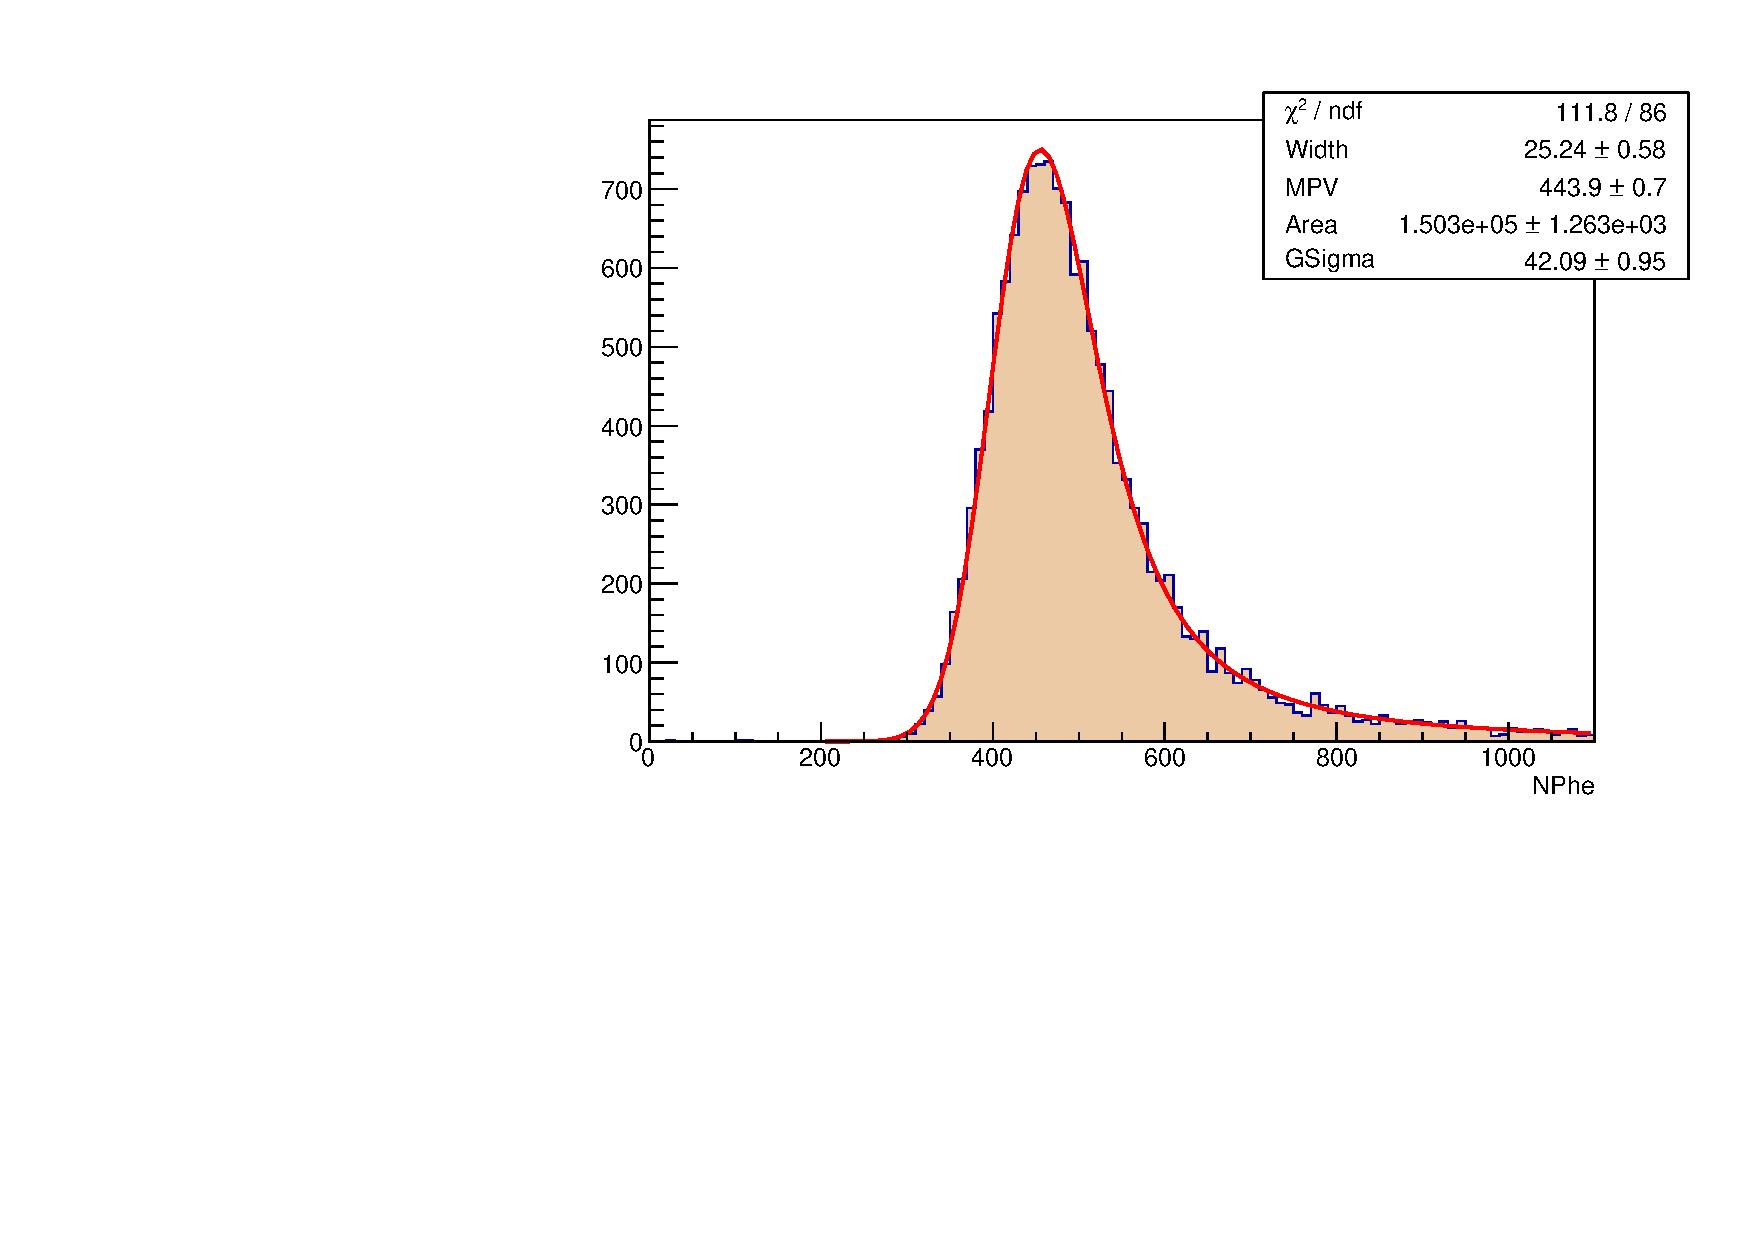
\includegraphics[width=.45\textwidth]{Physics/DetectorConcepts/Figs/NPHE_FCC.pdf}
\caption{Number of photo-electrons recorded in a small GRAiNITA prototype, 
where the ZnWO$_4$ grains are immersed in a heavy liquid to increase the density of the medium. 
Left: Cosmic-ray muons with ZnWO$_4$ grains immersed in ethylene-glycol (from Ref.~\cite{Barsuk_2024}). 
Right: Muon tracks from a beam test at CERN with ZnWO$_4$ grains 
immersed in LST~Fastloat (density = 2.8\,g/cm$^3$)~\cite{LST_Fastloat}.}
\label{fig:NPHE}
\end{figure}

\subsection{Hadron calorimeters}

\subsubsection{Scintillator tiles}

One of the considered hadron calorimeter designs is a non-compensating sampling calorimeter based on the ATLAS TileCal~\cite{ATLAS:2024bxb}, 
with steel as absorber and plastic scintillating tiles as active material. 
The light from the scintillator is collected and transported to the SiPMs 
located outside the calorimeter via WLS fibres, as shown in Fig.~\ref{fig:HCAL-Tile-module}. 

\begin{figure}[h]
\centering
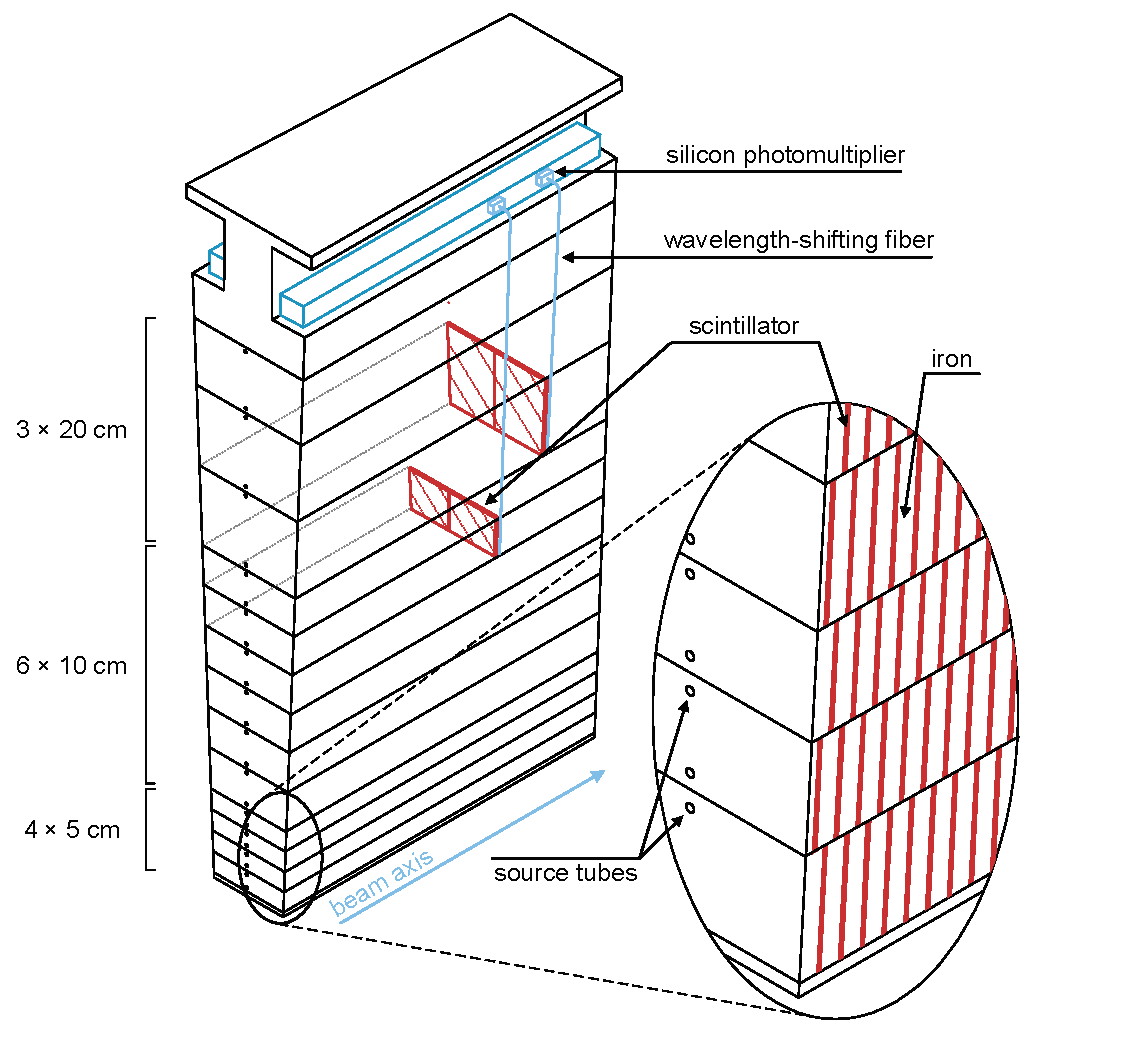
\includegraphics[width=0.5\linewidth]{Physics/DetectorConcepts/Figs/Allegro-HCAL-Tile-module-drawing-new4.pdf}
\caption{HCAL tile module concept. 
Each module consists of 13 radial layers of scintillating tiles with different radial extension (5, 10, and 20\,cm), 
and each radial layer is divided into two tiles in azimuth (hatched red). 
Scintillation light is brought to SiPMs at the outer radius via WLS fibres. 
In the $z$ direction, tiles are read out in groups of 3 or~4.}
\label{fig:HCAL-Tile-module}
\end{figure}

The radial orientation of the tiles and the light collection via the WLS fibres along the tile edges allow a hermetic implementation in $\phi$.
The location of the photodetectors and their associated electronics in the modules' girder at the outside radius 
makes them serviceable during collider shutdown periods. 
It also embeds the calibration system with movable radioactive $^{137}$Cs photon sources that can pass through all calorimeter cells~\cite{Blanchot:2020lyh}.

The proposed design uses 5\,mm low-carbon steel absorber plates interleaved with 3\,mm plastic scintillating tiles. 
The barrel is segmented into 128 modules in $\phi$ and 13 radial layers 
(of different depths: four of 5\,cm, six of 10\,cm, and three of 20\,cm, as shown in Fig.~\ref{fig:HCAL-Tile-module}). 
Each layer is divided in $\phi$ in two longitudinal read-out compartments. 
In each compartment, the tiles are read out in groups of three or four along the $z$ axis, 
which leads to a cell granularity $\Delta\phi \times \Delta\theta$ of $24.5 \times 22$\,mrad$^2$ at normal incidence. 
Steel-scintillator technology is also being considered for the end-cap hadron calorimeter. 

The performance of the tile HCAL, evaluated with a sliding window clustering algorithm, is shown in Fig.~\ref{fig:HCAL-Tile-resolution}. 
The optimisation of the calorimeter details, including the choice of the absorber and scintillating materials, as well as their segmentation, is ongoing.  
These R\&D studies are coordinated by the DRD6 WP3 (task~3.3.2), including the characterisation of perspective scintillating materials, 
like PEN and PET~\cite{CondeMuino:2023uzm}, and the light collection from scintillating tiles via WLS fibres with SiPM photodetectors~\cite{Schliwinski:2687718}.

\begin{figure}[ht]
\centering
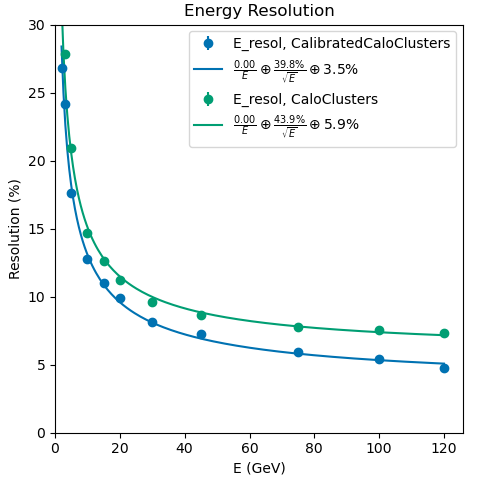
\includegraphics[width=0.5\linewidth]{Physics/DetectorConcepts/Figs/Allegro-HCAL-compare-clusters-E-resol.png}
\caption{HCAL tile energy resolution for hadron clusters.}
\label{fig:HCAL-Tile-resolution}
\end{figure}

A complementary approach is also being explored, 
with the so-called SiPM-on-Tile technology and with front-end electronics embedded into the active layers of a steel sandwich structure. 
The SiPMs are integrated into the electronics PCBs, which also hold read-out ASICs, power distribution, and a LED-based calibration system. 
Reflector-wrapped scintillator tiles are glued onto the PCB, with a dimple leaving space for the SiPMs underneath, which read each tile individually.

While the ATLAS-style geometry offers easier access and space for service routing, 
including cooling for a calorimeter placed outside the coil, 
the SiPM-on-Tile approach is the natural choice for calorimeter systems entirely inside the solenoid, such as in the CLD concept, 
where radial compactness (especially in the barrel) is strictly mandated by cost considerations. 
The technology was originally developed by the CALICE Collaboration;
a scalable prototype with 22\,000 channels was built and has been successfully tested in beams since 2018~\cite{CALICE:2022uwn}.
The main challenge in the adaptation to FCC-ee lies in coping with the continuous readout 
(i.e., without power-pulsing) 
and with the much higher rate, bandwidth, power, and cooling requirements, 
without compromising granularity and compactness. 

The R\&D  has common challenges with other concepts based on embedded electronics 
and is pursued in the framework of the WP1 of the DRD6 Collaboration. 
The SiPM-on-Tile technology is currently being applied in a large scale in the CMS HGCAL, a detector with 280\,000 tiles.
Although the CMS HGCAL has to address radiation hardness and other challenges not present at FCC-ee, 
it has more relaxed performance and compactness requirements, 
and remains more than an order of magnitude smaller in terms of channel count than, e.g., the CLD HCAL.

\subsubsection{Gaseous detectors}

Gaseous detector technologies with two-dimensional transverse segmentation are also pursued as read-out options for hadron calorimeters. 
Proof-of-principle elements have been tested using GEM and micromegas detectors, 
and larger prototypes with glass RPCs have been built and successfully tested, 
with up to 500\,000 channels~\cite{Baulieu:2015pfa,Adams:2016por}. 
Granularities finer than with tiles are easily achievable, 
but to maintain the designs cost-effective and to limit read-out power consumption, 
trade-offs must be found between energy and space information. 
The channel amplitude is encoded in one or two bits only, hence the name digital or semi-digital HCAL.

The related R\&D is pursued both in the DRD6 (`calorimeters') and in the DRD1 (`gas detectors') projects. 
The challenges of data concentration, powering, and cooling are shared with other ECAL and HCAL technologies with embedded readout. 
The quest for improving the detection technologies themselves, in terms of rate capability and stability, 
is common with R\&D for muon detectors, 
and both face the imperative of replacing the currently used gas mixtures with high global warming factors 
by more eco-friendly solutions. 

\subsubsection{Dual readout}

A fibre-sampling Dual-Readout (DR) calorimeter~\cite{dualreadoutfibrecalo} can, in principle, 
be used as a single system for electromagnetic and hadron showers. 
This option is considered in the IDEA concept, 
with a calorimetric section made of a dual-readout, longitudinally unsegmented and fully projective, fibre-sampling calorimeter, 
providing both electromagnetic and hadron shower measurements.
Another option is to use this technology as a hadron calorimeter behind an electromagnetic section based on crystals, 
as discussed in Section~\ref{sec:Segmented-crystals}.

Alternate rows of scintillating and Cherenkov (clear) fibres are inserted in capillary tubes made of brass or iron. 
Each fibre is individually read out with a SiPM. 
In order to significantly reduce the number of readout channels, the analogue grouping of 4--8 SiPM signals is foreseen. 
The optimal granularity is different if the detector has to provide both electromagnetic and hadronic shower measurements or just the latter. 
The present choice (1\,mm fibres in 2\,mm capillary tubes) is designed to address both.

\begin{figure}[ht]
\centering
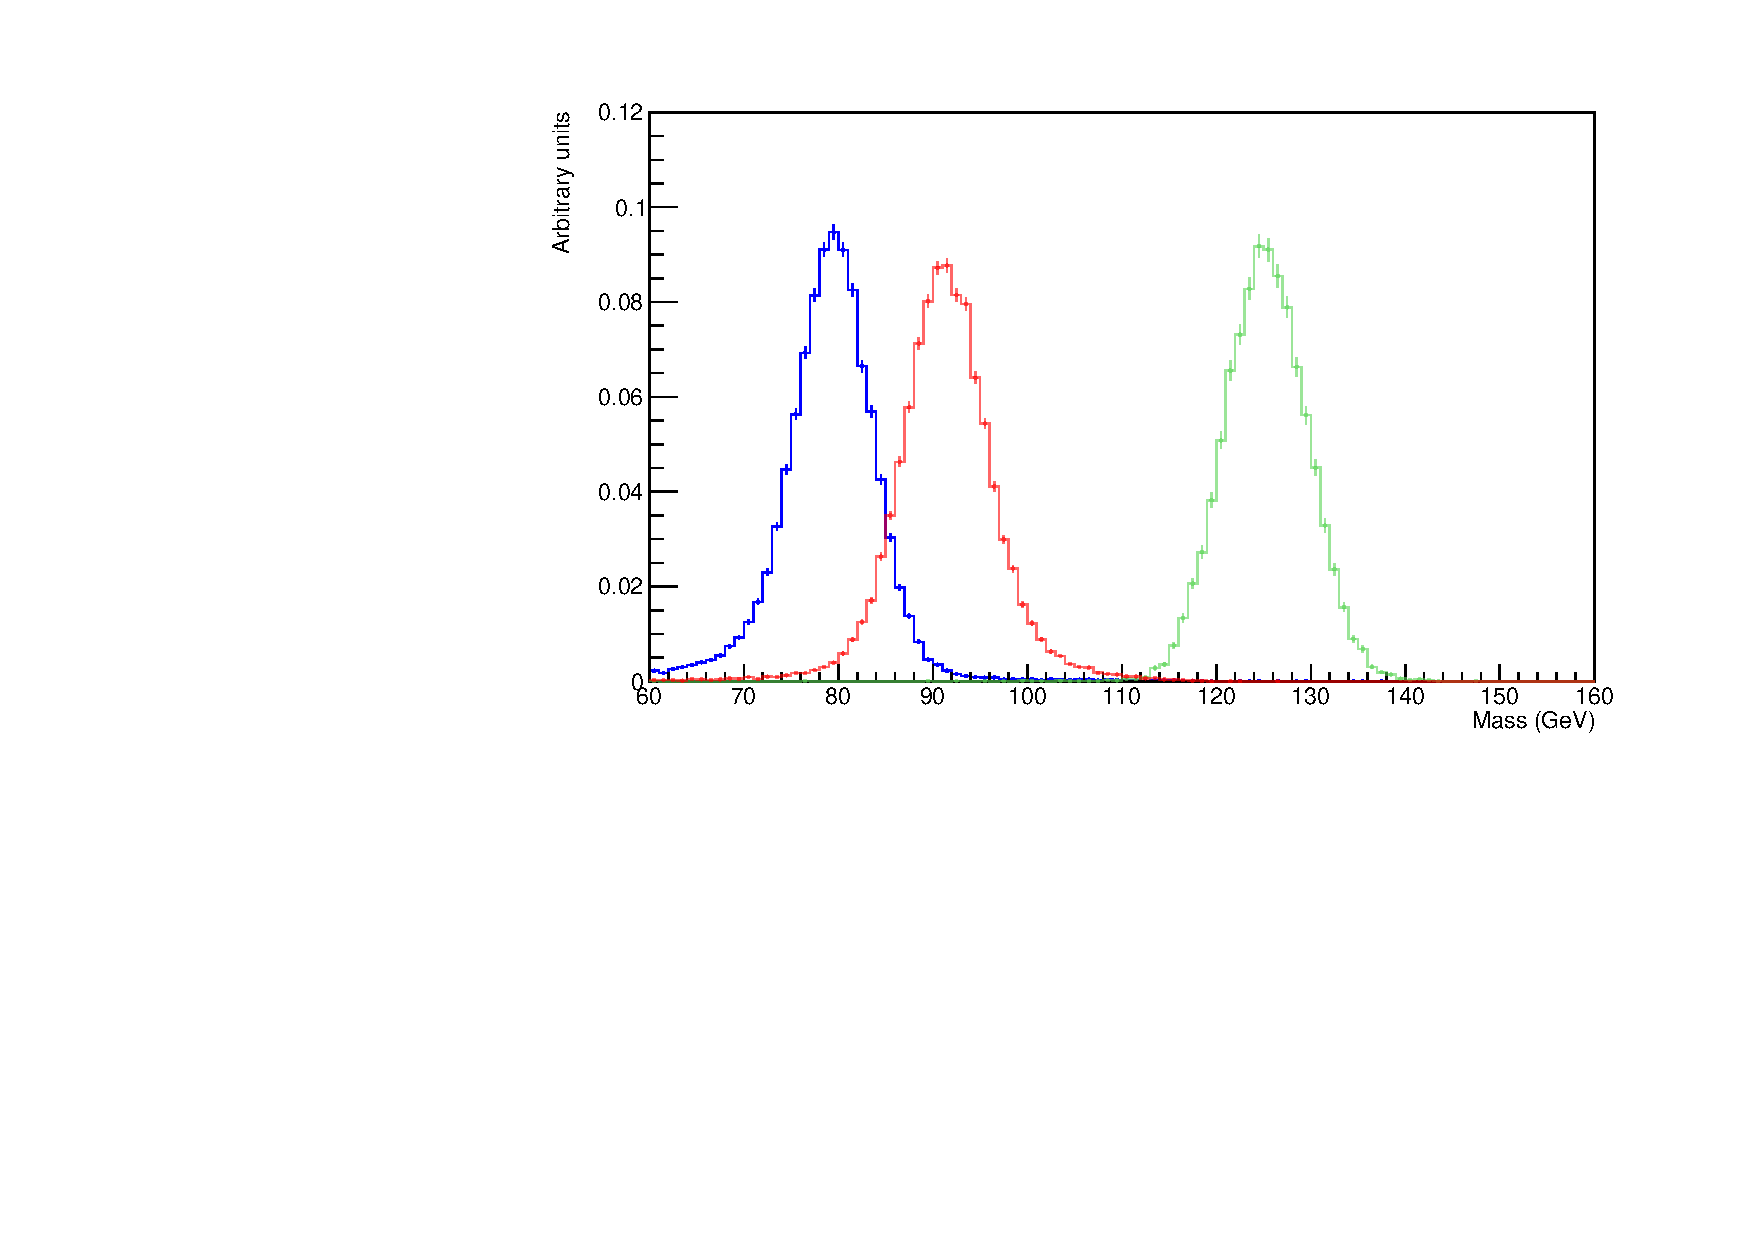
\includegraphics[width=0.5\textwidth]{Physics/DetectorConcepts/Figs/FibreHCal-WZH2jj.pdf}
\caption{From Ref.~\cite{Pezzotti:2021jxh}. Invariant mass distributions of \PW (blue), \PZ (red), and \PH (green) hadronic decays, from $\epem \to \PWp\PWm$ and $\PZ\PH$ events
fully simulated  and reconstructed at $\sqrt{s} = 240$\,GeV in a dual-readout fibre-sampling calorimeter.
To highlight the detector performance, semileptonic \PQb decays are excluded. 
}
\label{fig:DR-WZH2jj}
\end{figure}

The hadron energy resolution is estimated to be about $30\%/\sqrt{E}$, with a negligible constant term. 
The expected separation reachable for the \PW, \PZ and \PH hadronic decays is shown in Fig.~\ref{fig:DR-WZH2jj},
obtained with a stand-alone simulation and subsequent reconstruction of the DR calorimeter, 
and excluding semi-leptonic decays~\cite{Pezzotti:2021jxh}.
Similar studies show that this detector can provide excellent stand-alone electron-pion separation.
Moreover, the RD52 lead prototype obtained an efficiency of about 99\% in identifying electron showers, 
for a rejection ratio of charged-pion showers higher than 500~\cite{Akchurin:2014zna}.

Advances in solid-state light sensors, such as SiPMs, have opened the way for high transverse granularity,
which gives the detector the capability to determine shower angular positions at the mrad level, or better. 
In the present design, without a crystal-based electromagnetic calorimeter in front, 
the 1\,mm diameter fibres are placed in an iron absorber matrix, at a distance (apex to apex) of 1.5--2 mm. 
The lateral segmentation could be pushed down to the mm level, 
largely enhancing the resolving power for close-by showers, with a significant impact expected, for example, 
on the isolation and reconstruction of $\PGt \to \PGr \PGn$ final states. 
For the setup with crystals in front, the segmentation of the DR sections remains to be optimised.

The high photo-detection efficiency of SiPMs should lead to light yields of $\mathcal{O}(100)$ photo-electrons per GeV, 
for both the scintillation and Cherenkov signals, 
which guarantees a stand-alone EM resolution close to $10\%/\sqrt{E}$. 
Readout ASICs providing time information with about 100\,ps resolution 
may allow the reconstruction of the longitudinal shower position with a resolution of about 5\,cm.

On the other hand, the large number and density of channels require an innovative readout architecture for efficient information extraction. 
Both charge integration and waveform sampling ASICs are available on the market and candidates for early testing have been identified.
A first implementation of a scalable readout system is well-advanced.
Looking further ahead, digital SiPMs (dSiPMs) should allow a significant simplification of the readout architecture, 
but the technology is not yet sufficiently mature. 
A specific R\&D programme has been approved for the 2025--2026 period.

The mechanical assembly and integration of a system with $\mathcal{O}(10^8)$ sensitive elements 
require the development of a robust and engineered procedure. 
A scalable mechanical solution has been conceived for both non-projective and projective modules. 
A small ($\sim$\,$10 \times 10 \times 100$\,cm$^3$) EM prototype has been built,
based on the gluing of capillary tubes.
This procedure is being used for the construction of a hadron calorimeter prototype 
(of size $\sim$\,$60 \times 60 \times 250$\,cm$^3$) that should be completed by mid 2025. 
Alternative approaches, for both mechanical assembly and readout architecture, are being investigated within DRD6.

\begin{figure}[h]
\centering
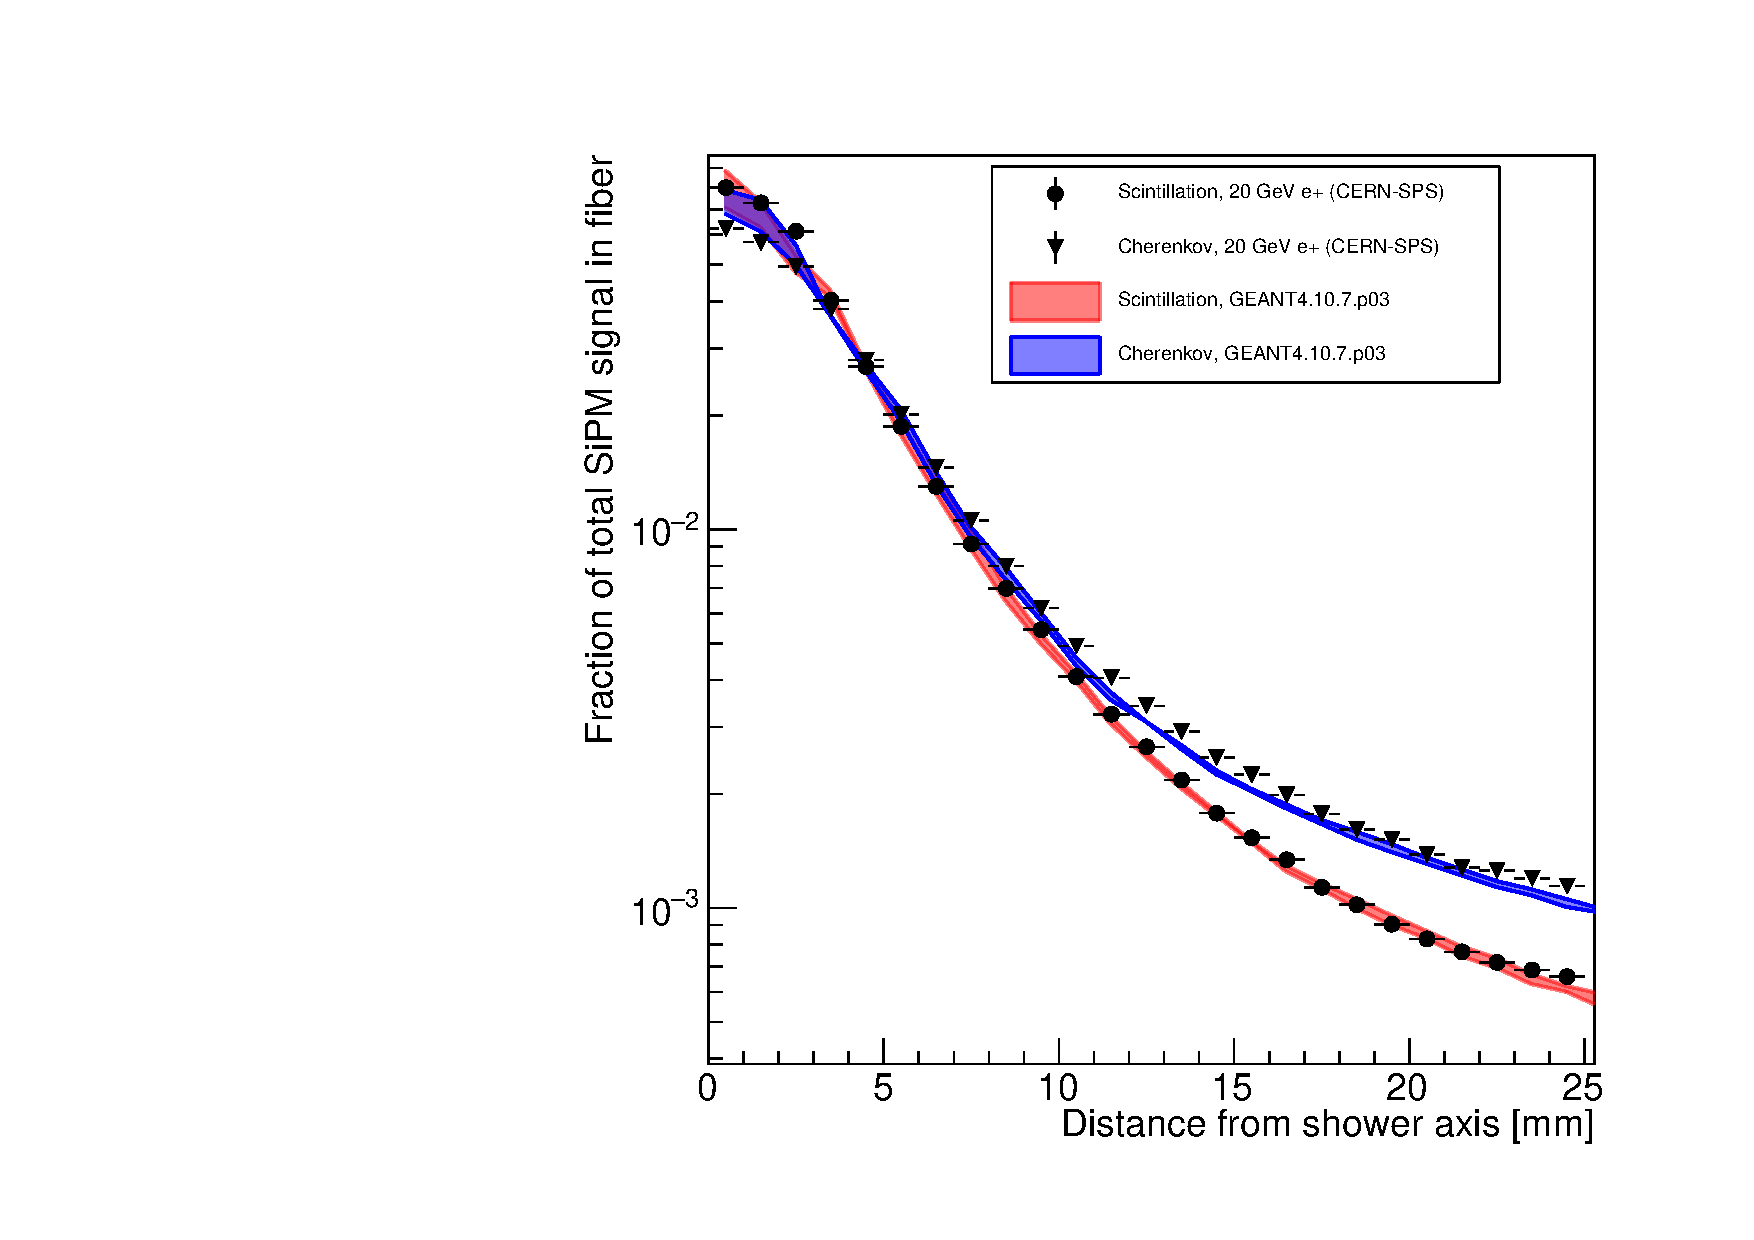
\includegraphics[width=0.45\textwidth]{Physics/DetectorConcepts/Figs/emShowerProfile.pdf}
\caption{Lateral shower profile of positrons with an energy of 20\,GeV. 
The black circles (triangles) refer to the scintillation (Cherenkov) options. 
The red and blue bands correspond to the simulation predictions for the scintillation and Cherenkov signal, respectively.}
\label{fig:emShowerProfile}
\end{figure}

The EM prototype was tested with beam at the CERN SPS and the results (Fig.~\ref{fig:emShowerProfile}) show that simulations model the instrumental effects well.
The performance in the reconstruction of the properties of both hadron and EM showers
is sufficient to retain the possibility of an integrated dual-readout solution based on fibre-sampling only, 
for the calorimetric system of an FCC-ee experiment. 
The huge amount of information made available by the fibre SiPM readout is well suited to take advantage of deep-learning algorithms. 

\subsection{Coil}

Conceptual studies of 2\,T superconducting solenoid variants have been concluded for the CLD, IDEA, and ALLEGRO FCC-ee detector concepts. 
From a conceptual perspective, the CLD solenoid is similar to that of CMS, 
with the calorimeters located inside the solenoid bore. 
A relatively high energy density is targeted, for the purpose of limiting the weight of the cold mass, with various benefits, 
in particular regarding the overall cost and easier transport from the manufacturer to CERN. 
For the IDEA and ALLEGRO concepts, the solenoid is located inside the hadron calorimeter and the free-bore diameter is substantially smaller. 
The advantage of this variant is that the cold-mass weight is reduced, 
albeit at the cost of requiring high particle transparency of the cold mass, thermal shields, and vacuum vessel. 
The design of thin, low-mass magnet systems is discussed in Ref.~\cite{fcc-ee-cdr}. 
Representative field maps are shown in Fig.~\ref{fig:CLD+IDEASolenoid} 
and typical design parameters are shown in Table \ref{tab:solenoidVariants}.

\begin{figure}[ht]
\centering
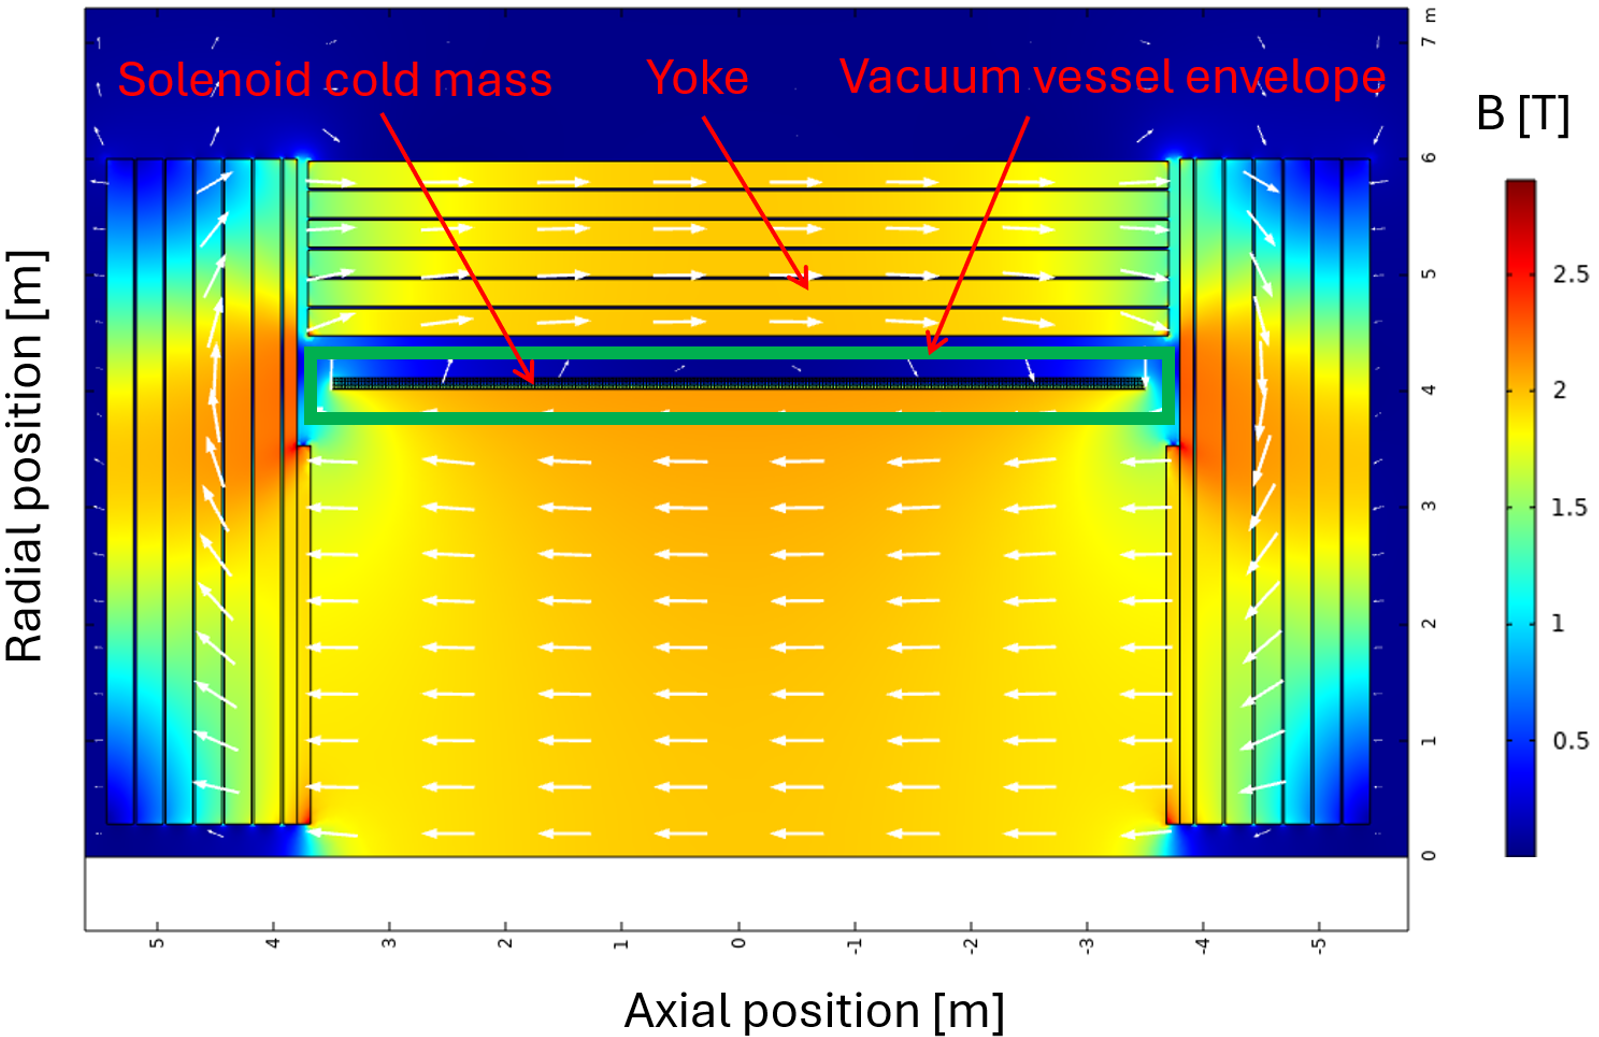
\includegraphics[width=0.47\linewidth]{Physics/DetectorConcepts/Figs/CLD_fieldmap_180924.png}
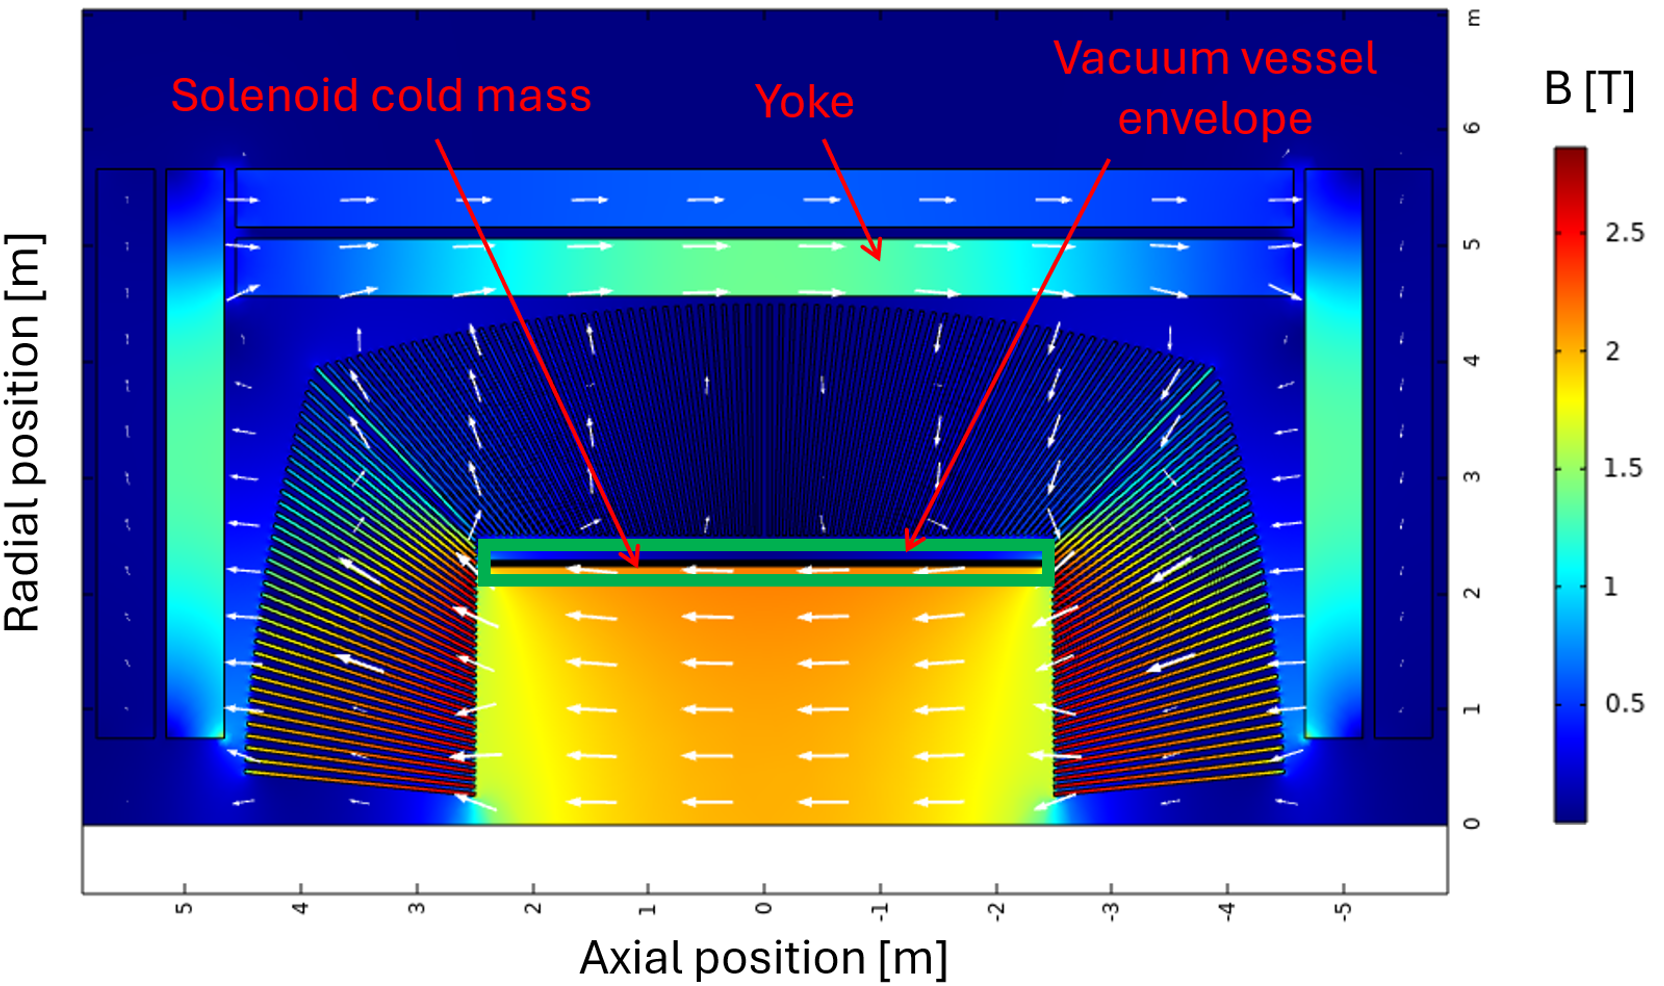
\includegraphics[width=0.52\linewidth]{Physics/DetectorConcepts/Figs/IDEA_fieldmap_180924.png}
\caption{Field maps of the CLD (left) and IDEA (right) detector magnets in the ($r,z$) view, featuring 2\,T in the free bore.}
\label{fig:CLD+IDEASolenoid}
\end{figure}

\begin{table}[ht] 
\caption{Overview of typical design parameters of the different solenoid variants.}
\label{tab:solenoidVariants}
\centering
\begin{tabular}{ c c c c}
\toprule
Variant & Stored magnetic & Cold mass & Energy density \\
        & energy (MJ) & weight (t) & (kJ/kg) \\
\midrule
CLD & 590 & 52 & 11.4 \\\
IDEA & 130 & 10.6 & 12.3 \\
Allegro & 250 & 22 & 11.4 \\
\bottomrule
\end{tabular}
\end{table}

For each variant, a relatively high energy density, of about 12\,kJ/kg, is targeted, 
a value comparable to what was previously shown in the CMS solenoid and the Bess--Polar solenoid~\cite{Yamamoto:2002dwn}. 
This energy density poses challenges for quench protection and cold-mass mechanics but, 
relying on technological solutions previously demonstrated for the ATLAS, CMS, and Bess--Polar solenoids, 
no setbacks were identified. 
The baseline is to build the solenoids with reinforced aluminium-stabilised low-temperature superconductors. 
These conductors have been successfully applied in many detector magnet projects worldwide over the past decades 
and they meet the technical requirements of the FCC detector magnets, 
regarding the field ranges, the free bores, the transparency to particles, and the mechanics and stability. 
The preferred technology is co-extrusion of Nb-Ti/Cu Rutherford cable in a high purity aluminium stabiliser. 
This technology offers the best characteristics for coil quench protection and coil stability, with an indirect cooling. 
Strong mechanical properties can be reached using either Ni-doped high-purity aluminium stabiliser, 
or aluminium alloy profiles electron-beam-welded to the coextruded aluminium-stabilised superconductor. 
It should be noted that this assumes the commercial availability of reinforced aluminium-stabilised Nb-Ti conductor. 
At the time of the conclusion of the conceptual cold-mass studies, 
it became clear that companies that had historically made this conductor type commercially available had discontinued production.

As an alternative to aluminium-stabilised Nb-Ti conductor technology, preliminary studies were made 
concerning the implications of aluminium-stabilised high-temperature-superconducting (HTS) conductors. 
The use of HTS brings interesting benefits, 
such as potentially allowing a higher operating temperature and, thus, reduced cryogenic operating costs.
The implications for capital costs, cold mass mechanics, quench detection and protection are, however, 
not yet fully understood and characterised. 
This technology requires further R\&D before it can be concluded that it is a reliable alternative to the Nb-Ti conductor.
Two manufacturing methods are considered for the aluminium-stabilised HTS: 
co-extrusion in high-purity aluminium profiles and soft soldering in copper-plated aluminium profiles. 
As the HTS are produced in thin tapes, several HTS conductor technologies are envisaged: 
stacks of tapes, Roebel cables, and conductor on round core (CORC\textsuperscript{\textregistered}) conductors.

An Experimental Magnets Committee was established by CERN in 2023 to address the R\&D needs of detector magnet projects 
and to resolve identified issues regarding the availability of technologies and facilities needed 
to manufacture superconductors for detector magnets. 
An ongoing programme is targeting to establish access to a co-extrusion line that would allow R\&D and prototyping, 
both with low- and high-temperature aluminium-stabilised superconductors. 
In addition to the CERN effort, specific R\&D for an HTS solenoid for IDEA/ALLEGRO is currently in progress at INFN-LASA. 

\subsection{Cryostat}
\label{sec:Cryostat}

The use of carbon composite technologies for cryostat construction is being studied in an R\&D programme in the CERN EP Department. 
In collaboration with industry, a 1\,m carbon composite cryostat prototype has recently been developed, 
as shown in Fig.~\ref{fig:CarbonCryostatPrototype}. 
The manufacturing procedure, based on a wet filament winding process, 
ensures helium leak-tightness at cryogenic temperatures without the need for a metallic liner.

\begin{figure}[ht]
\centering
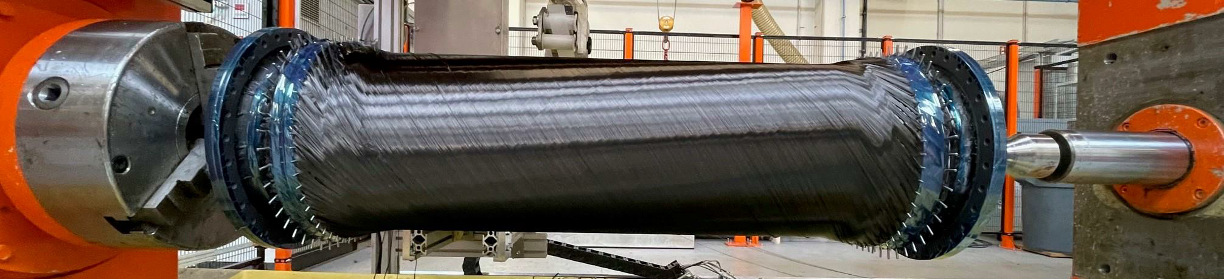
\includegraphics[width=0.95\linewidth]{Physics/DetectorConcepts/Figs/CarbonCryostarPrototype.png}
\caption{Full liner-less tank demonstrator, 1\,m length, 0.3\,m diameter, and 5\,mm wall thickness. 
Manufacturing process: filament wet-winding, non-crossing, out-of-autoclave curing.}
\label{fig:CarbonCryostatPrototype}
\end{figure}

Recent developments to support large-scale production (larger than 5\,m in diameter and length), 
include the refinement of the winding process and the development of a toughened epoxy resin to enhance resistance to microcracking.
Additionally, a novel technique has been developed to wind each ply of material without fibre crossings, 
minimising porosity and further improving microcrack resistance. 
Promising helium leak tests at low temperatures indicate that strict cryogenic standards can be met for detector operations. 

The ability of cryostat vessels to resist structural instability (buckling) under compressive loads poses an additional challenge. 
The use of a full carbon honeycomb as a replacement for aluminium honeycomb is being explored. 
Initial prototypes have undergone extensive testing, including thermal expansion and dimensional stability assessments, 
underscoring the suitability of carbon honeycomb for large, buckling-sensitive cryostat walls. 

The combination of a leak-tight carbon wall with the full carbon honeycomb core 
represents a promising design direction for next-generation HEP cryostats. 
A preliminary study, using the ALLEGRO detector concept as an example, revealed 
a 64\% reduction in the material budget and a 30\% reduction in wall thickness for buckling-sensitive cryostat walls 
compared to an aluminium sandwich design, 
with a thermal expansion coefficient one order of magnitude lower while maintaining comparable mechanical properties.

\subsection{Muon system}

Several technologies are under consideration for use in detector muon systems at FCC-ee, 
including $\mu$-RWELL~\cite{MUON:micro-RWELL}, resistive plate chambers~\cite{SANTONICO1981377}, 
resistive Micromegas~\cite{ALEXOPOULOS2011110}, scintillators, drift tubes, and combinations thereof. 
Apart from muon identification, these systems can offer capabilities for tail catching of calorimeter showers, 
identification of long-lived particles by providing tracking with good position resolution, or independent triggers.

Three $\mu$-RWELL layers are currently implemented in the IDEA design, in both the barrel and end-cap regions, 
housed within the iron yoke that closes the detector magnetic field. 
The $\mu$-RWELL chambers provide 2D space point measurements with a few hundred micron precision. 
In order to benefit from industrial production capabilities of this technology, 
a modular design is adopted with basic $\mu$-RWELL `tiles' with an active area of $50 \times 50$\,cm$^2$
and a readout strip pitch of about 1\,mm, 
enabling a sufficient spatial resolution of about 400\,$\mu$m while limiting the number of readout channels to 1000 per tile.
The choices of detector tile size, strip pitch and width are a compromise between 
the largest $\mu$-RWELL detector that can be industrially mass-produced 
and the maximum input detector capacitance that can be tolerated in terms of signal over noise ratio by the front-end electronics.

Table~\ref{tab:barrel-muon} lists the dimensions, the number of basic $\mu$-RWELL tiles, 
and the readout channels of the three muon stations of the IDEA detector. 
In total, including the barrel and the end-cap muon stations, 
the system comprises about 5800 $\mu$-RWELL tiles with about 6 million readout channels. 

\begin{table}[ht]
\centering
\caption{Dimensions of the three IDEA barrel muon stations, 
together with the number of detector tiles and the corresponding number of readout channels.}
\label{tab:barrel-muon}
\begin{tabular}{@{}cccccccc@{}}
\toprule
Station &
  \begin{tabular}[c]{@{}c@{}}Radius\\ {(}m{)}\end{tabular} &
  \begin{tabular}[c]{@{}c@{}}Length\\ {(}m{)}\end{tabular} &
  \begin{tabular}[c]{@{}c@{}}Strip pitch\\ {(}mm{)}\end{tabular} &
  \begin{tabular}[c]{@{}c@{}}Strip length\\ {(}mm{)}\end{tabular} &
  \begin{tabular}[c]{@{}c@{}}Area\\ {(}m$^2${)}\end{tabular} &
  \begin{tabular}[c]{@{}c@{}}\# of\\ tiles\end{tabular} &
Channels \\ 
\midrule
1 & 4.52 & 9.0   & 1 & 500 & 260 & 1040 & 1\,040\,000 \\
2 & 4.88 & 9.0   & 1 & 500 & 280 & 1120 & 1\,120\,000 \\
3 & 5.24 & 10.52 & 1 & 500 & 350 & 1400 & 1\,400\,000 \\ 
\bottomrule
\end{tabular}
\end{table}

The geometries and material of both the barrel and the end-caps have been implemented in the \textsc{Geant4} full simulation of the muon system. 
The implementation of algorithms for digitisation and clustering will follow in the next step of the study. 
Since the $\mu$-RWELL technology has not yet been used to build a full detector system, 
a vigorous R\&D programme to study integration issues will be carried out in the coming years. 
The detailed layout of the detector, together with all its services, will have to be accurately developed. 
The optimisation of the basic $\mu$-RWELL tile, including gas gap, diamond like carbon layer resistivity, and gas amplification, 
has started~\cite{MUON:test-beam,MUON:resistivity} and is expected to be finalised to match the requirements of the IDEA muon system by 2027. 
The $\mu$-RWELL R\&D is performed in synergy with the WP1 of DRD1~\cite{MUON:DRD1}. 
Another important aspect of this R\&D programme is the design and development of dedicated front-end electronics based on a custom-made ASIC.

\subsection{Luminosity measurement}
\label{sec:lumi}

For the precise measurement of cross sections, the integrated luminosity must be determined with high precision. 
Ambitious goals have been formulated on the measurement precision: 
$10^{-4}$ or better on the \emph{absolute} luminosity 
and $5 \times 10^{-5}$ or better on the \emph{relative} luminosity between energy scan points. 
At FCC-ee, the wide-angle diphoton process, $\epem \to \PGg\PGg$, is statistically relevant 
and provides a promising complement to the traditional low-angle Bhabha scattering process, $\epem \to \epem$.
For both processes, the definition of the geometrical precision constitutes an important source of systematic uncertainty.

As discussed in Section~\ref{sec:PhysPerf_gammagamma}, 
the $\PGg\PGg$ final state places a requirement on the accuracy of the lower limit of the polar angle acceptance at the 8\,$\mu$rad level, 
corresponding to 20\,$\mu$m at 2.5\,m from the IP. 
For each of the proposed ECAL solutions, R\&D is needed on how to obtain such construction precision. 
Complementary methods to determine the acceptance in-situ with this precision or better 
are under development and alluded to in Section~\ref{sec:PhysPerf_gammagamma}.
Likewise, studies are needed on how to ensure that the efficiency of observing the $\PGg\PGg$ final state 
can be understood to the required precision over the wide detector acceptance.

For the measurement of low-angle Bhabha scattering, 
the luminosity calorimeters (LumiCals) are located close to the beam pipe, 
where they are neighbouring the complex Machine Detector Interface region (Chapter~\ref{sec:mdi}). 
Placed in front of the compensating solenoids, the LumiCals are at only $\sim$\,1.1\,m from the IP. 
In this region, space is severely limited and a very compact design is called for. 
The Bhabha cross section falls very steeply, as $1/\theta^3$, with $\theta$ being the scattering angle, 
resulting in very challenging tolerances on the definition of the geometrical precision at the $\mathcal{O}$(1\,$\mu$m) level.

\subsubsection{LumiCal design}
\label{sec:LumiCal}

Based on experience from LEP~\cite{OPAL:1999clt,Bederede:1995pc}
and from past linear collider studies \cite{Behnke:2013lya,CLIC:2016zwp,Abramowicz:2018vwb}, 
compact SiW sandwich calorimeters are proposed as luminosity monitors for the measurement of low-angle Bhabha scattering. 
The calorimeters are designed as cylindrical devices assembled from stacks of identical SiW layers. 
This simple geometry facilitates the control of construction and metrology tolerances to the necessary micron level, 
as emphasised by the OPAL experiment~\cite{OPAL:1999clt}.
The monitors are centred around the outgoing beam directions in the severely limited space available,
in front of the compensating solenoids, which extend to $|z| \simeq 1.2$\,m from the IP. 
The monitor design is illustrated in Fig.~\ref{fig:luminometer}, where the main physical dimensions are also given. 
The design includes 25 layers, each comprising a 3.5\,mm tungsten plate, equivalent to one radiation length, 
and a Si-sensor plane inserted in the 1\,mm gap. 
In the transverse plane, the Si sensors are finely partitioned into pads. 
The proposed segmentation features 32 divisions, both radially and azimuthally, 
for 1024 readout channels per layer, or 25\,600 channels in total for each calorimeter. 
A solution with a four times finer azimuthal segmentation is also under consideration.

\begin{figure}[ht]
\centering
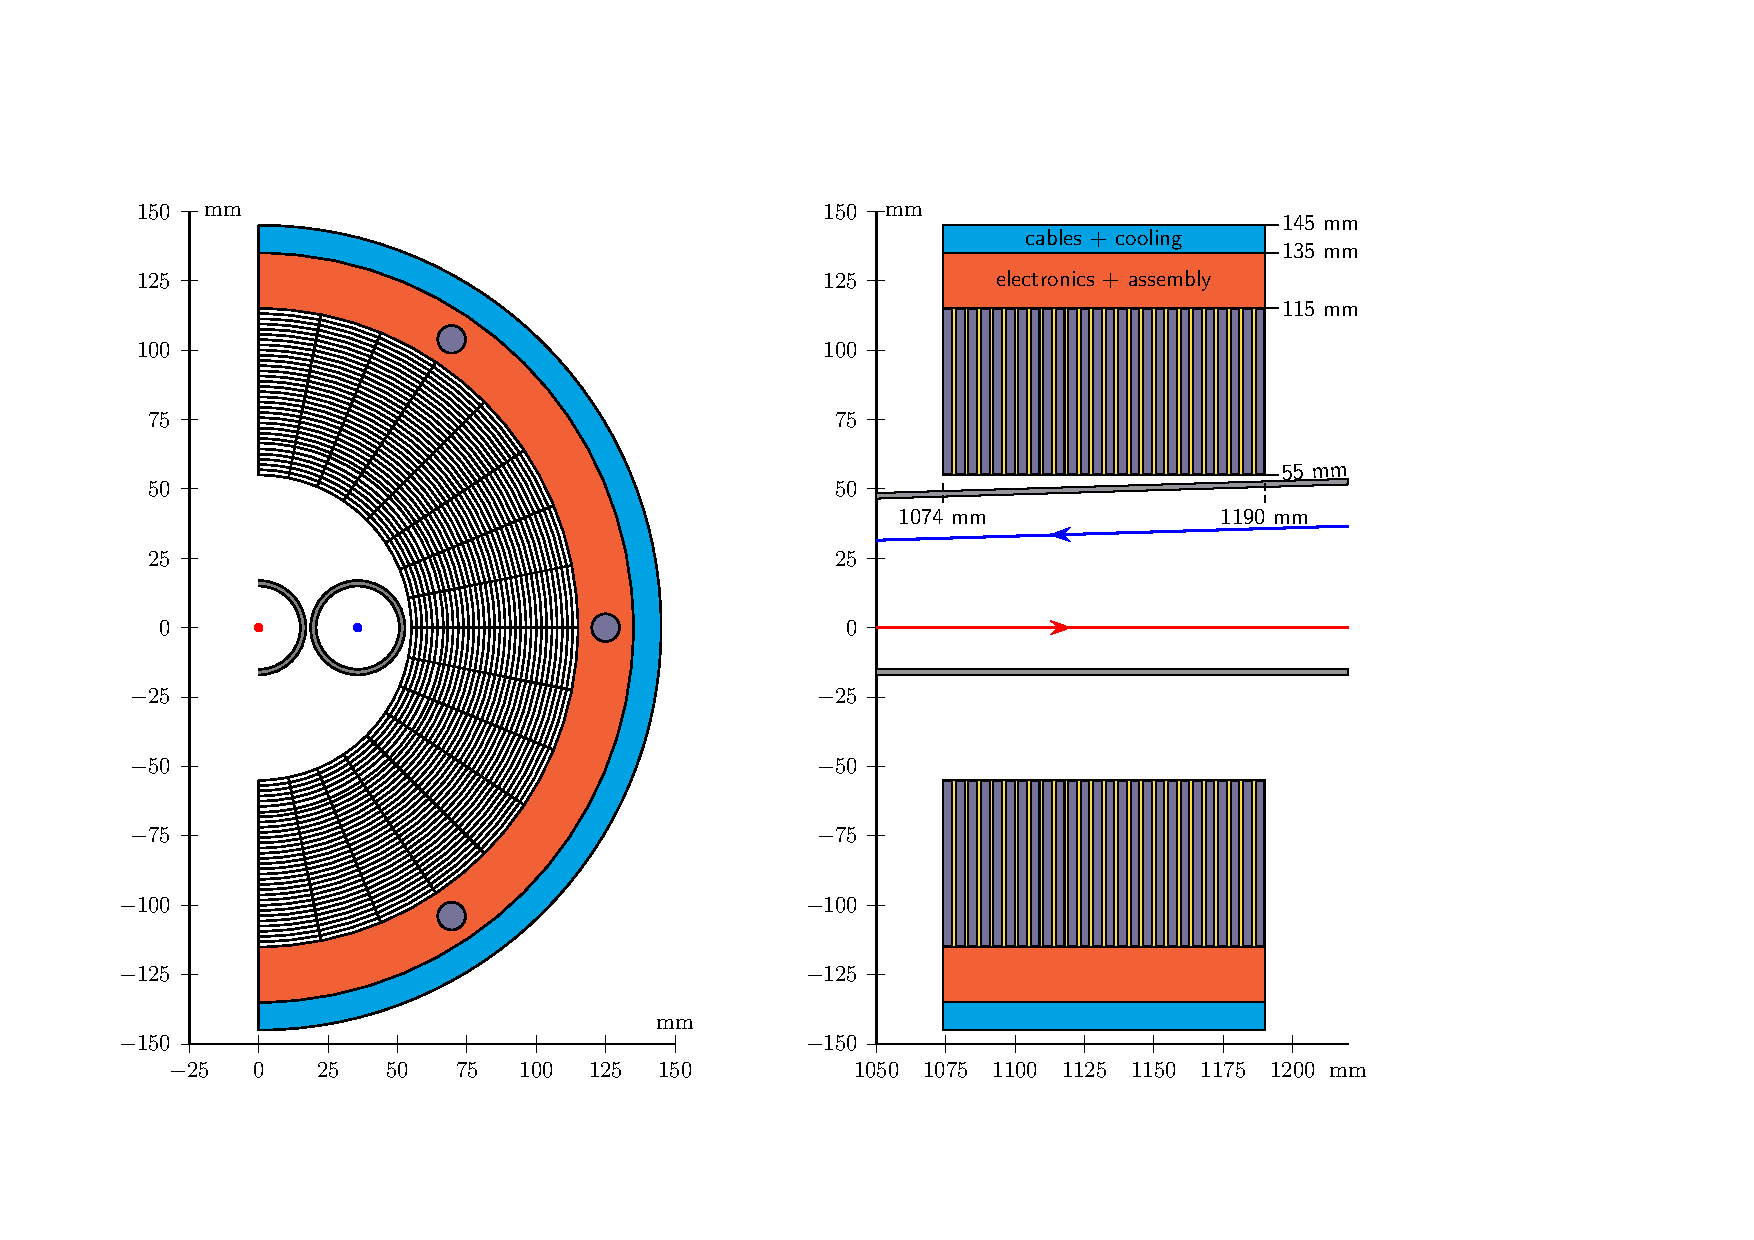
\includegraphics[width=0.8\textwidth]{Physics/DetectorConcepts/Figs/LumiCal.pdf}
\caption{Front view (left) and top view (right) of the luminosity calorimeter, 
centred around the outgoing beam direction (shown as a red arrow). 
A possible  segmentation of the Si pads is seen in the front view. 
Surrounding the sensitive region are regions for front-end electronics (red), and for cables and cooling (blue). 
The top view shows the interleaved silicon-tungsten layer structure.}
\label{fig:luminometer}
\end{figure}

A 30\,mm uninstrumented region at the outer circumference is reserved for services (front-end electronics, cables, and cooling), 
as well as for the physical structures (likely including precision dowels and bolts) needed for the assembly of the SiW sandwich. 
Overall, the proposed design is very compact, each calorimeter weighing only about 65\,kg. 
An example of the integration of the LumiCals with the MDI and the detector system 
is shown in Figs.~\ref{fig:cooling_cones} and~\ref{fig:support_cyl}, in Chapter~\ref{sec:mdi}.

The Si-sensor pads are connected to front-end electronics positioned at radii immediately outside the sensors. 
To minimise the occurrence of pile-up events, it is desirable to read out the sensors at the bunch-crossing rate. 
This constraint calls for the development of readout electronics with an $\mathcal{O}$(20\,ns) shaping time. 
From experience with similar electronics development~\cite{FCAL:FLAME}, 
a power budget of 5\,mW per readout channel has been estimated, for a total of 130\,W per calorimeter, to be removed by cooling. 
For the required geometric precision, the temperature needs to be controlled to within a tolerance of 1\,$^\circ$C.

The goal of $10^{-4}$ precision on the absolute luminosity measurements translates into a required precision of 
$\mathcal{O}$(1\,$\mu$m) on the radial dimensions of the calorimeters 
and of $\mathcal{O}$(100\,$\mu$m) on the distance between the two calorimeters.

First full simulation studies of the LumiCals have been performed using 45.6\,GeV electrons. 
They show that the proposed geometry covers the polar angle region between 53 and 98\,mrad for fully contained showers, 
corresponding to a cross section of 28\,nb at the \PZ-pole energy. 
With a sampling fraction of 1.1\%, the calorimeters have an energy resolution of 3.2\%, corresponding to $22\%/\sqrt{E}$. 
The intrinsic resolution on the radial coordinate of showers is found to be 75\,$\mu$m at a $z = 1100$\,mm reference plane, 
considerably better than the contribution of about 120\,$\mu$m 
from multiple scattering of the primary electrons in the 2\,mm of beam pipe material traversed at shallow angles.

The feasibility of the proposed design has been demonstrated in part, over the last two decades, 
by work of the FCAL R\&D Collaboration, which had been specialising in technologies for very-forward calorimeters at linear colliders. 
A five-layer prototype with a similar sandwich structure was built and successfully tested in a beam test~\cite{Abramowicz:2018vwb}, 
and a dedicated readout system based on a custom-designed readout chip was prepared~\cite{FCAL:FLAME,FCAL:FLAME2}. 

Much work is needed towards a consolidated LumiCal design that satisfies the many severe requirements. 
Important future steps include:

\begin{itemize}
\item 
Engineering-level study of the proposed detector assembly method, which involves precision dowels and through-going bolts. 
This study must take into account the required $\mathcal{O}$(1\,$\mu$m) geometrical precision on the radial coordinate.
\item 
Realistic estimate of the space needed for services at radii outside the sensitive region. 
This region shall be kept as transparent as possible by the use of lightweight materials, to minimise particle interactions.
\item 
Design of a procedure for maintaining and monitoring the geometric accuracy of the monitors via precise metrology and alignment.
\item 
Design of a cooling system allowing control of a constant and uniform temperature over the monitors. 
The required tolerances have to be developed.
\item 
Re-evaluation of the expected radiation dose based on the final collider parameters 
and assessment of whether existing sensor technologies are adequate or further sensor R\&D is required.
\item 
Design of compact low-power readout electronics that preferentially allows readout at the 50\,MHz bunch-crossing rate, 
including transmission of signals away from the detectors. 
The system developed by the FCAL Collaboration may be a good starting point.
\item
Further full simulation studies to optimise the design of the detector.
\end{itemize}

\subsection{Outlook}

During the Feasibility Study, 
the detector designer community confirmed and enhanced its engagement and commitment 
to support a few complete detector concepts 
and to develop innovative detectors capable of delivering the required physics performance. 
The FCC-ee detectors have to meet unprecedented performance requirements 
in order to match the expected statistical precision and discovery physics potential. 
These requirements are, in many respects, complementary to what was needed at HL-LHC: 
while radiation tolerance is not an issue, with few exceptions close to the beams, 
the demands on precision, efficiency, purity, transparency of trackers, 
and compactness of calorimeters are considerably more challenging. 
Even though the readout bandwidth requirements appear relaxed when compared to the situation at HL-LHC, 
the required rate capabilities far exceed those from past linear collider studies. 
These constraints significantly magnify the system design and integration challenges 
especially if material budget and dead space are to be kept at minimum.

The detector R\&D community has undergone a restructuring process, 
leading to the formation of DRD Collaborations to address these demands. 
While it is clear that these Collaborations will only be able to unfold their potential 
with an adequate ramp-up of resources, 
it is also important to emphasise that they must benefit from proper guidance 
through the detector conceptual activities in the FCC effort. 
In particular, it is crucial to continue to develop and maintain a powerful common software framework 
(Chapter~\ref{sec:software}), including full-simulation tools, 
in view of establishing and evolving the link between the detector concepts, on the one hand, 
and technological R\&D, prototype design and construction, and ultimately test-beam data analysis, on the other. 
It will be essential that this common framework be adopted by the DRD teams, 
to optimise the subsystem inclusion in the FCC-ee detector simulation studies. 
Indeed, realistic geometries and digitizers will be essential to assess physics performance, 
as well as to compare with prototypes and test-beam data.

The detector community is well connected worldwide. 
The US and European roadmap processes, for example, 
have been well informed of each other and led to the formulation of overarching themes that are aligned to a large extent. 
This process is reflected in the ongoing integration of international groups and projects into the new DRD structure. 
Many of the proposals submitted to the DRD Collaborations target future Higgs factories and, 
among those, many specifically target FCC-ee. 
Given the current FCC-ee timeline, the R\&D in the 2025--2027 period will give priority to conceptual and component studies, 
with system aspects in focus from the beginning, 
preparing the way to the possible development of prototypes and demonstrators 
during the subsequent three-year period (2028--2030), 
followed by the construction and test of realistic modules by 2035. 

The next phase of the FCC study will first capitalise on the developments made during the Feasibility Study 
regarding the full-simulation of the existing proto-detector concepts, 
to confront their simulated performance with the detector requirements from physics. 
This work will clarify if those physics-driven requirements are matched by the current proto-detector concepts 
and will point the way to alternative detector solutions.
Different detector configurations will then be studied to optimise both performance and cost. 
In parallel, the links to the DRD Collaborations will be tightened. 
Work towards the common goal of developing FCC-ee detector concepts will be encouraged, 
by giving the R\&D groups the necessary inputs and requirements from the FCC Feasibility Study, 
and by identifying their needs in terms of guidance and software tools. 

Several challenges, specifically needed for FCC-ee but maybe not included in the DRD programme, will also need to be addressed. 
For example:
\begin{itemize}
\item How to monitor the time-stability of the magnetic field map in the experiments at the $10^{-7}$ level 
(taking into account all magnetic elements, including compensating solenoids, etc.)?
\item How to achieve, possibly using a set of geometry systems, 
the accuracy on the knowledge of the alignment and surveying fiducials required for precision measurements 
(such as the luminosity measurement at low angles, the dilepton/diphoton cross section measurements at large angles, 
or the tau lepton lifetime measurement)?
\item Can cosmic-ray muons continue to be used for the global alignment of FCC detectors, 
despite the fact that they will operate in much deeper caverns than those of previous colliders?
\item Are there new detector technologies or configurations that would be particularly well-suited for specific FCC-ee measurements 
or that would be beneficial in view of improving the performance-to-cost ratio?
\end{itemize}

In the next few years, regular workshops will be organised with the DRD Collaborations, 
to evaluate possible design choices for detector subsystems, 
including their simulation, optimisation, demonstrators, and key engineering aspects, 
as well as to foster interactions and cross-fertilisation between interested institutes. 
Issues ranging from low-level readout architectures and engineering resources 
to larger-scale system integration, full-simulation-based optimisation, and high-level event reconstruction, 
will be addressed.
The goal will be to quantify the cost and performance (including flexibility aspects) of each specific design choice, 
always retaining a physics-driven perspective,
towards the timely delivery of conceptual design reports and full detector concepts proposals shortly after 2030. 
Reaching this ambitious goal will require an appropriate re-organisation 
and a significant injection of more (human and financial) resources in the project.